\section{Experiments}
\label{app:experiments}

\begin{experiment}
  In this experiment Goal~\ref{goal:homomorphism} is tested.
  \begin{itemize}
    \item \emph{$\aNH$ traverses the history by $-4$ to $\aNH'$}
    \item \emph{$\aNH'$ traverses the history by $+4$ to $\aNH''$}
  \end{itemize}
  By Goal~\ref{goal:homomorphism}, these traversals should be the same thing as \emph{$\aNH$ traversing by $0$} which is a no-op; therefore, $\aNH = \aNH''$.

  Firefox:
  \begin{figure}[H]
    \raisebox{-.5\height}{
      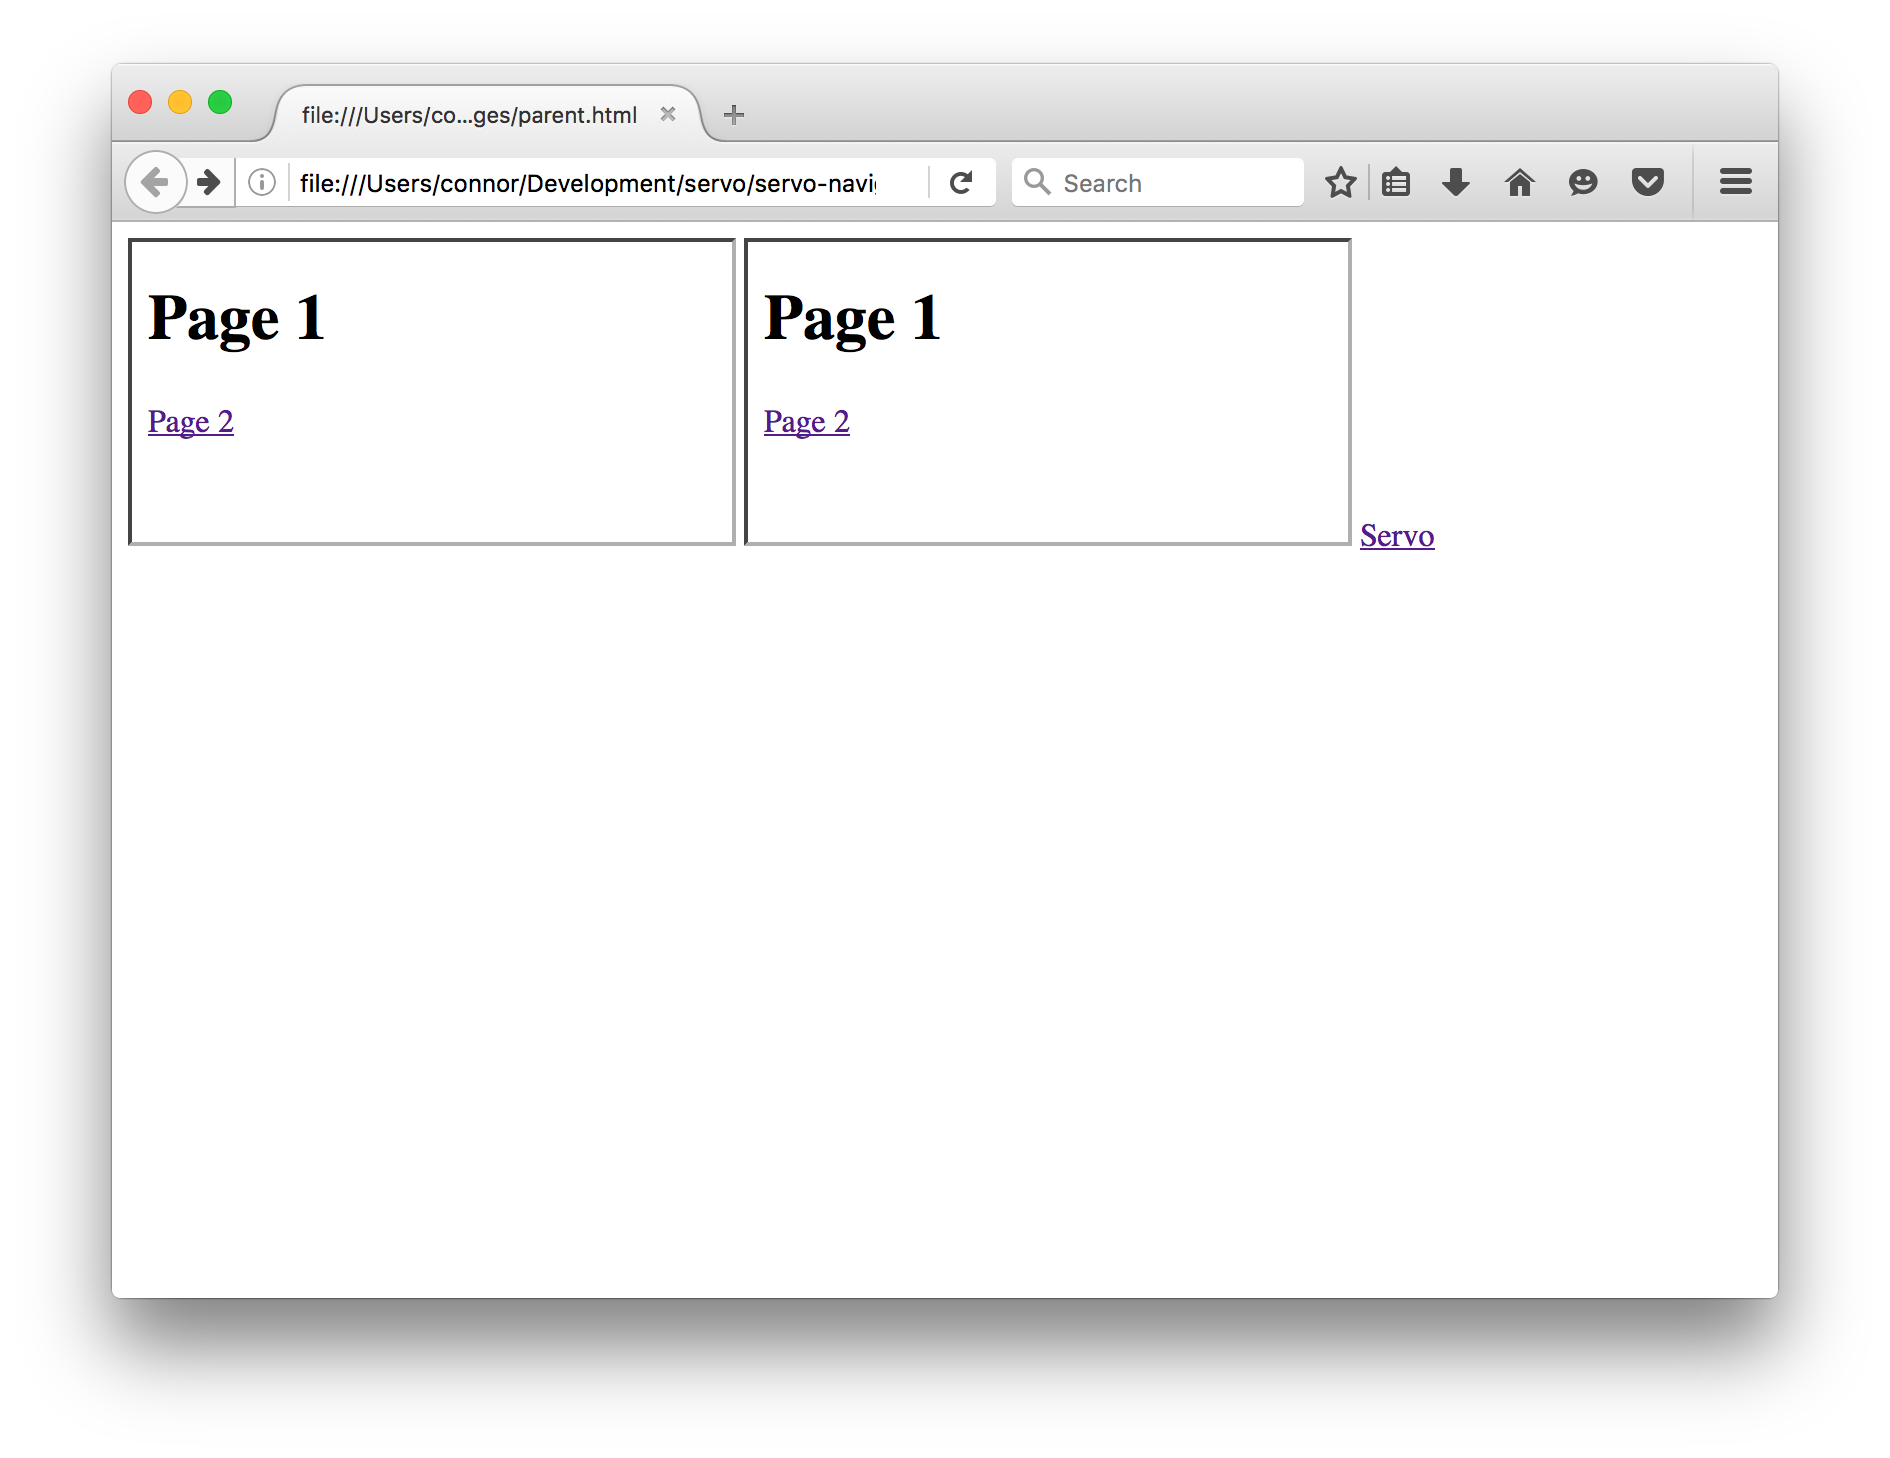
\includegraphics[width=.5\linewidth]{images/experiments/forwardback4/firefox/1.png}%
    }~\raisebox{-.5\height}{
      \begin{tikzpicture}
        \node[doc,active,fully](0) at (0,0){0};
        \node[doc,active,fully](1) at (1,-1){1};
        \node[doc,jshactive,fully](2) at (2,-2){2};
        \node[draw,dotted,fit=(0)]{};
        \node[draw,dotted,fit=(1)]{};
        \node[draw,dotted,fit=(2)]{};
        \draw[->](0)--(1);
        \draw[->](0)to[out=-20,in=90](2);
      \end{tikzpicture}
    }
    \caption{Initial State}
  \end{figure}

  Navigate document $1$ to Page 2:
  \begin{figure}[H]
    \raisebox{-.5\height}{
      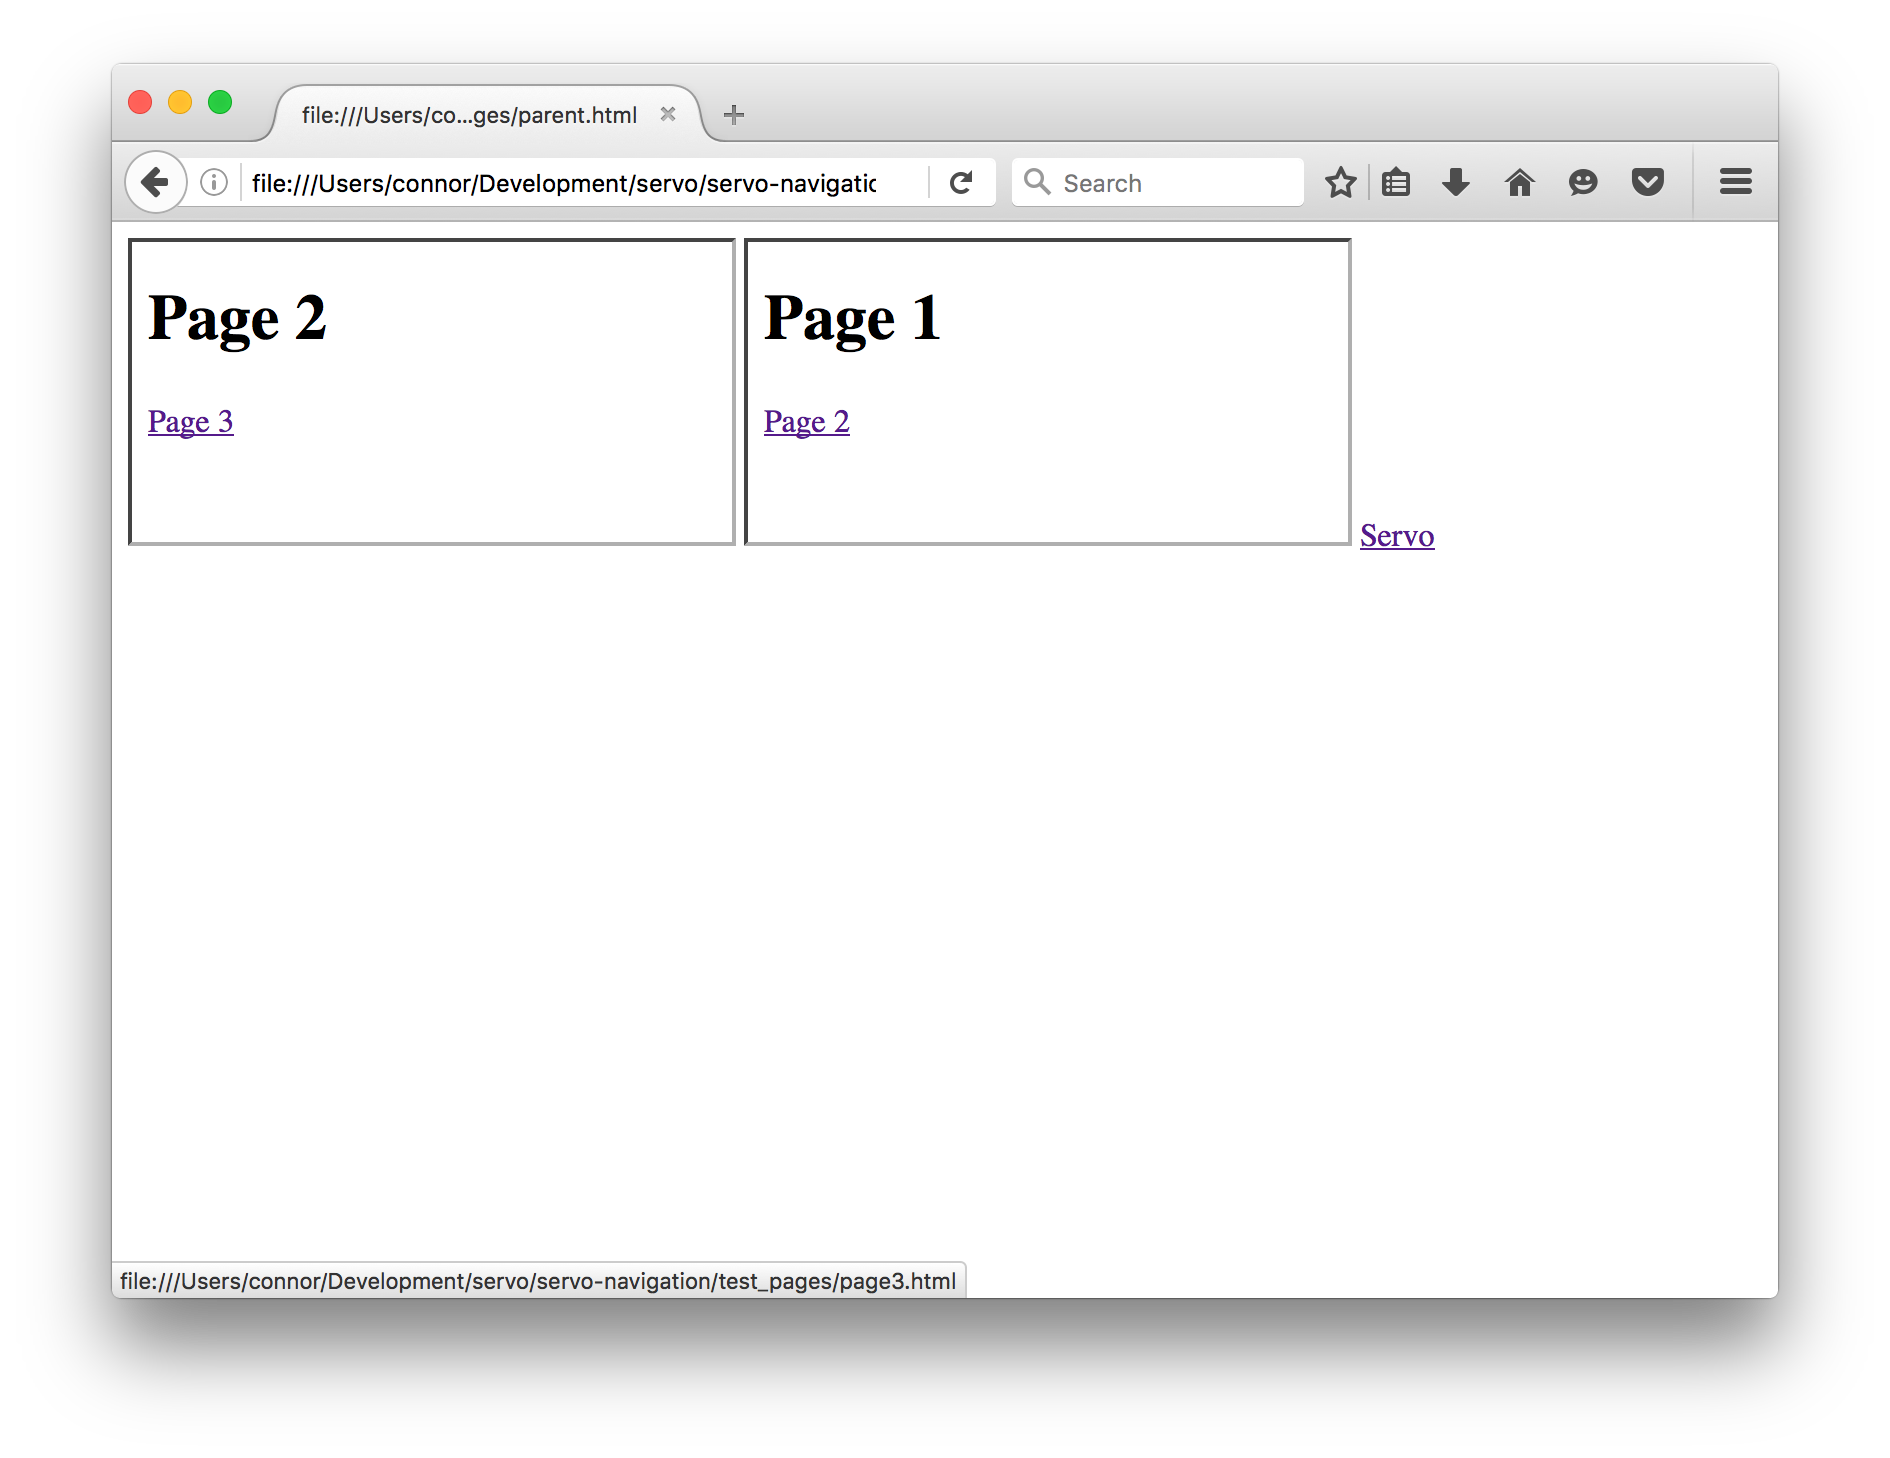
\includegraphics[width=.5\linewidth]{images/experiments/forwardback4/firefox/2.png}
    }~\raisebox{-.5\height}{
      \begin{tikzpicture}
        \node[doc,active,fully](0) at (0,0){0};
        \node[doc](1) at (1,-1){1};
        \node[doc,active,fully](2) at (2,-2){2};
        \node[doc,jshactive,fully](3) at (3,-1){3};
        \node[draw,dotted,fit=(0)]{};
        \node[draw,dotted,fit=(1)(3)]{};
        \node[draw,dotted,fit=(2)]{};
        \draw[->](0)--(3);
        \draw[->](0)to[out=-20,in=90](2);
      \end{tikzpicture}
    }
    \caption{Navigate document $1$ to Page 2.}
  \end{figure}

  Navigate document $3$ to Page 3:
  \begin{figure}[H]
    \raisebox{-.5\height}{
      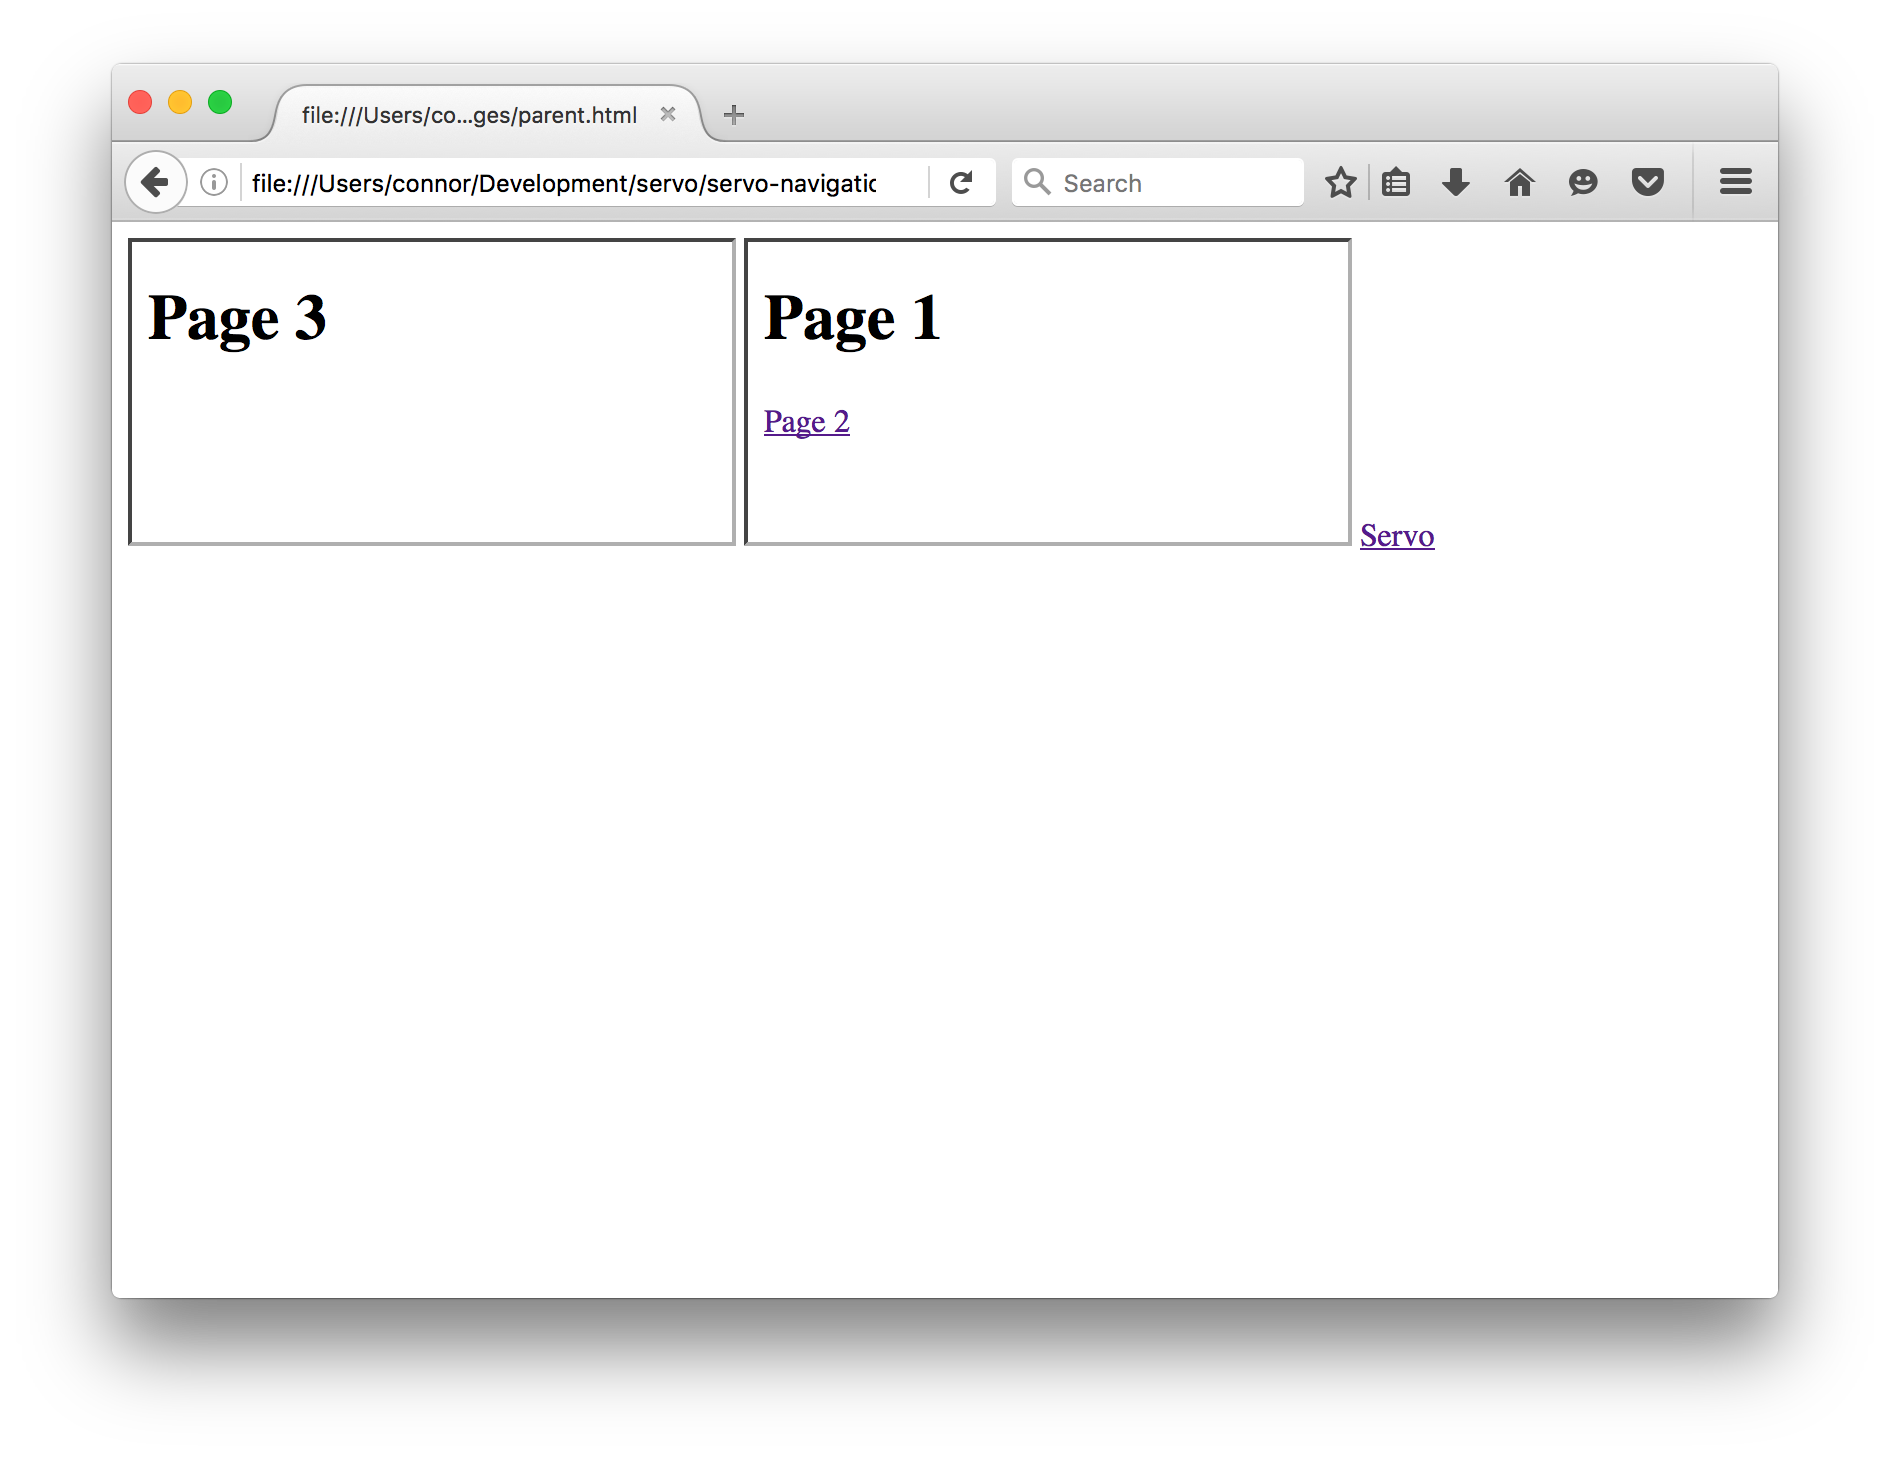
\includegraphics[width=.5\linewidth]{images/experiments/forwardback4/firefox/3.png}
    }~\raisebox{-.5\height}{
      \begin{tikzpicture}
        \node[doc,active,fully](0) at (0,0){0};
        \node[doc](1) at (1,-1){1};
        \node[doc,active,fully](2) at (2,-2){2};
        \node[doc](3) at (3,-1){3};
        \node[doc,jshactive,fully](4) at (4,-1){4};
        \node[draw,dotted,fit=(0)]{};
        \node[draw,dotted,fit=(1)(4)]{};
        \node[draw,dotted,fit=(2)]{};
        \draw[->](0)to[out=0,in=140](4);
        \draw[->](0)to[out=-20,in=90](2);
      \end{tikzpicture}
    }
    \caption{Navigate document $3$ to Page 3.}
  \end{figure}

  Navigate document $2$ to Page 2:
  \begin{figure}[H]
    \raisebox{-.5\height}{
      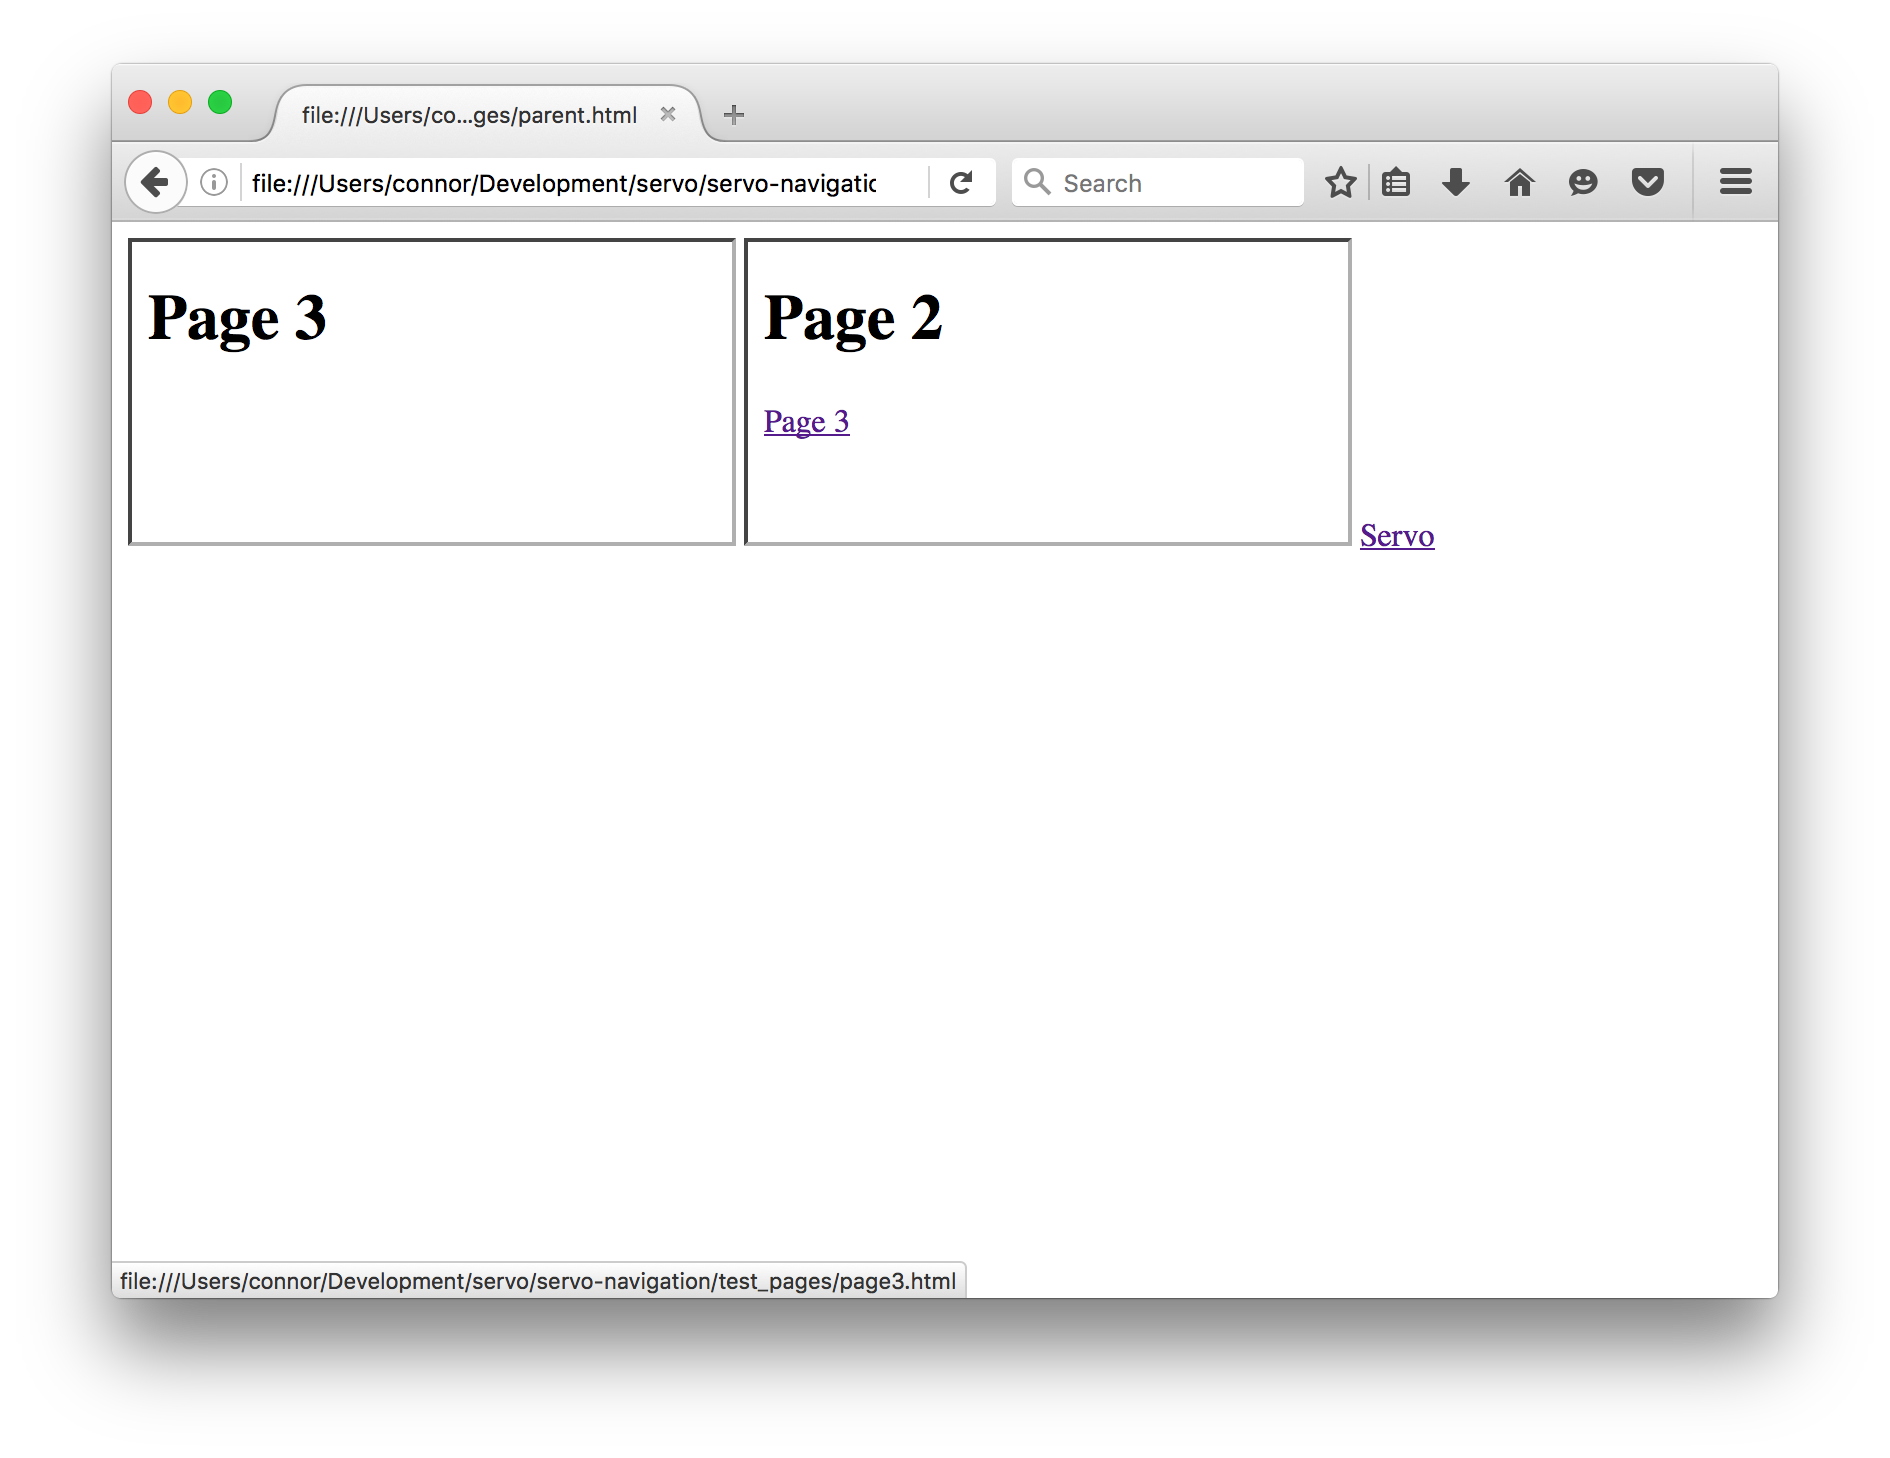
\includegraphics[width=.5\linewidth]{images/experiments/forwardback4/firefox/4.png}
    }~\raisebox{-.5\height}{
      \begin{tikzpicture}
        \node[doc,active,fully](0) at (0,0){0};
        \node[doc](1) at (1,-1){1};
        \node[doc](2) at (2,-2){2};
        \node[doc](3) at (3,-1){3};
        \node[doc,active,fully](4) at (4,-1){4};
        \node[doc,jshactive,fully](5) at (5,-2){5};
        \node[draw,dotted,fit=(0)]{};
        \node[draw,dotted,fit=(1)(4)]{};
        \node[draw,dotted,fit=(2)(5)]{};
        \draw[->](0)to[out=0,in=140](4);
        \draw[->](0)to[out=0,in=90](5);
      \end{tikzpicture}
    }
    \caption{Navigate document $2$ to Page 2.}
  \end{figure}

  Navigate document $5$ to Page 3:
  \begin{figure}[H]
    \raisebox{-.5\height}{
      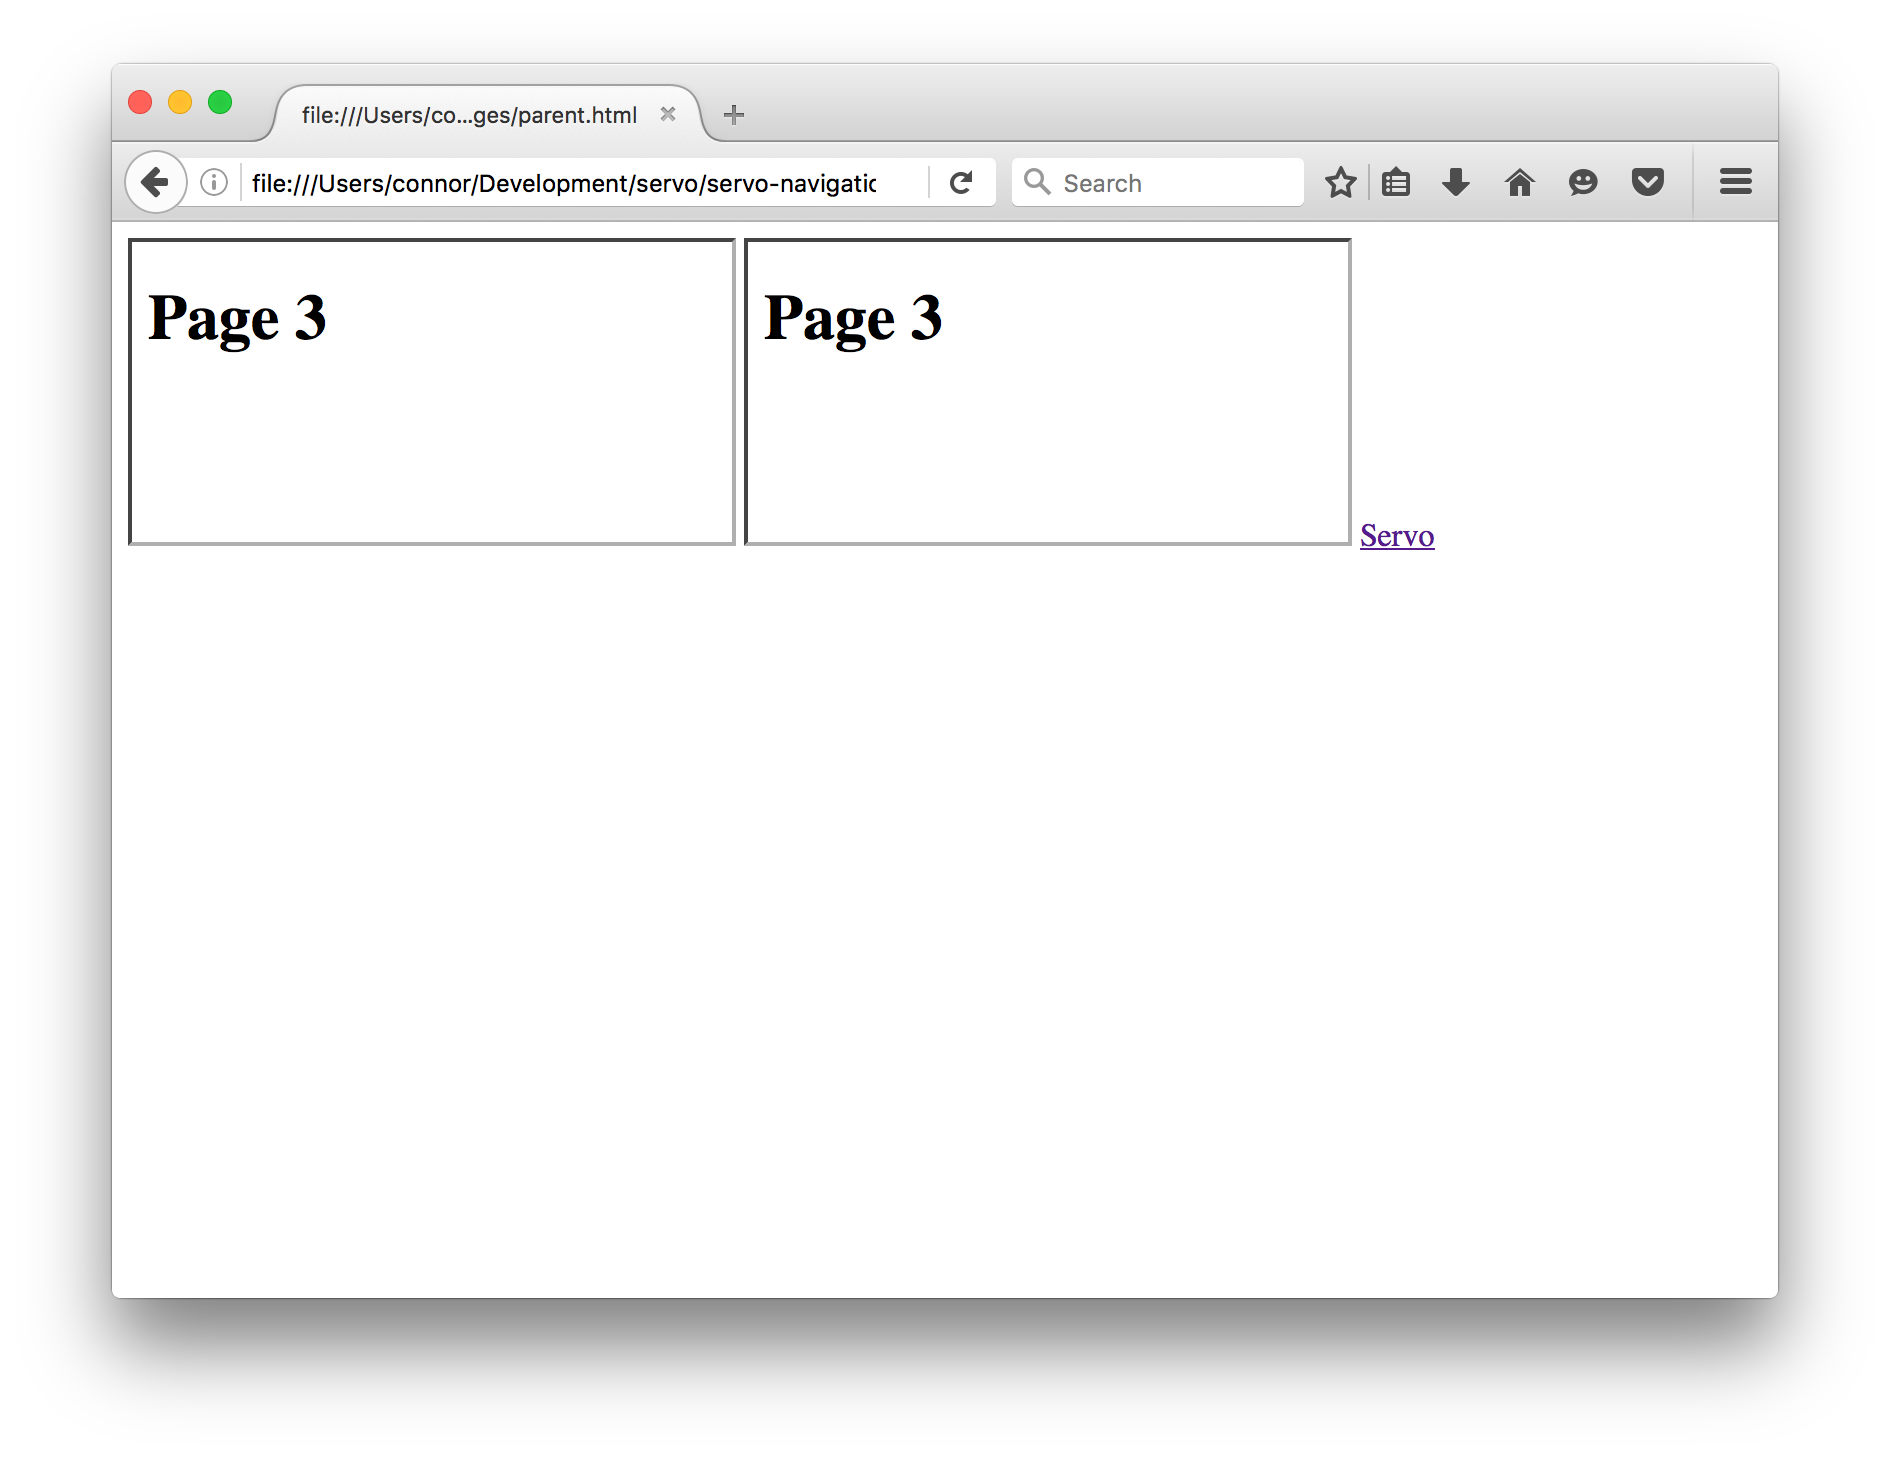
\includegraphics[width=.5\linewidth]{images/experiments/forwardback4/firefox/5.png}
    }~\raisebox{-.5\height}{
      \begin{tikzpicture}
        \node[doc,active,fully](0) at (0,0){0};
        \node[doc](1) at (1,-1){1};
        \node[doc](2) at (2,-2){2};
        \node[doc](3) at (3,-1){3};
        \node[doc,active,fully](4) at (4,-1){4};
        \node[doc](5) at (5,-2){5};
        \node[doc,jshactive,fully](6) at (6,-2){6};
        \node[draw,dotted,fit=(0)]{};
        \node[draw,dotted,fit=(1)(4)]{};
        \node[draw,dotted,fit=(2)(6)]{};
        \draw[->](0)to[out=0,in=140](4);
        \draw[->](0)to[out=0,in=120](6);
      \end{tikzpicture}
    }
    \caption{Navigate document $5$ to Page 3.}
  \end{figure}

  \emph{$\aNH$ traverses the history by $-4$ to $\aNH'$}:
  \begin{figure}[H]
    \raisebox{-.5\height}{
      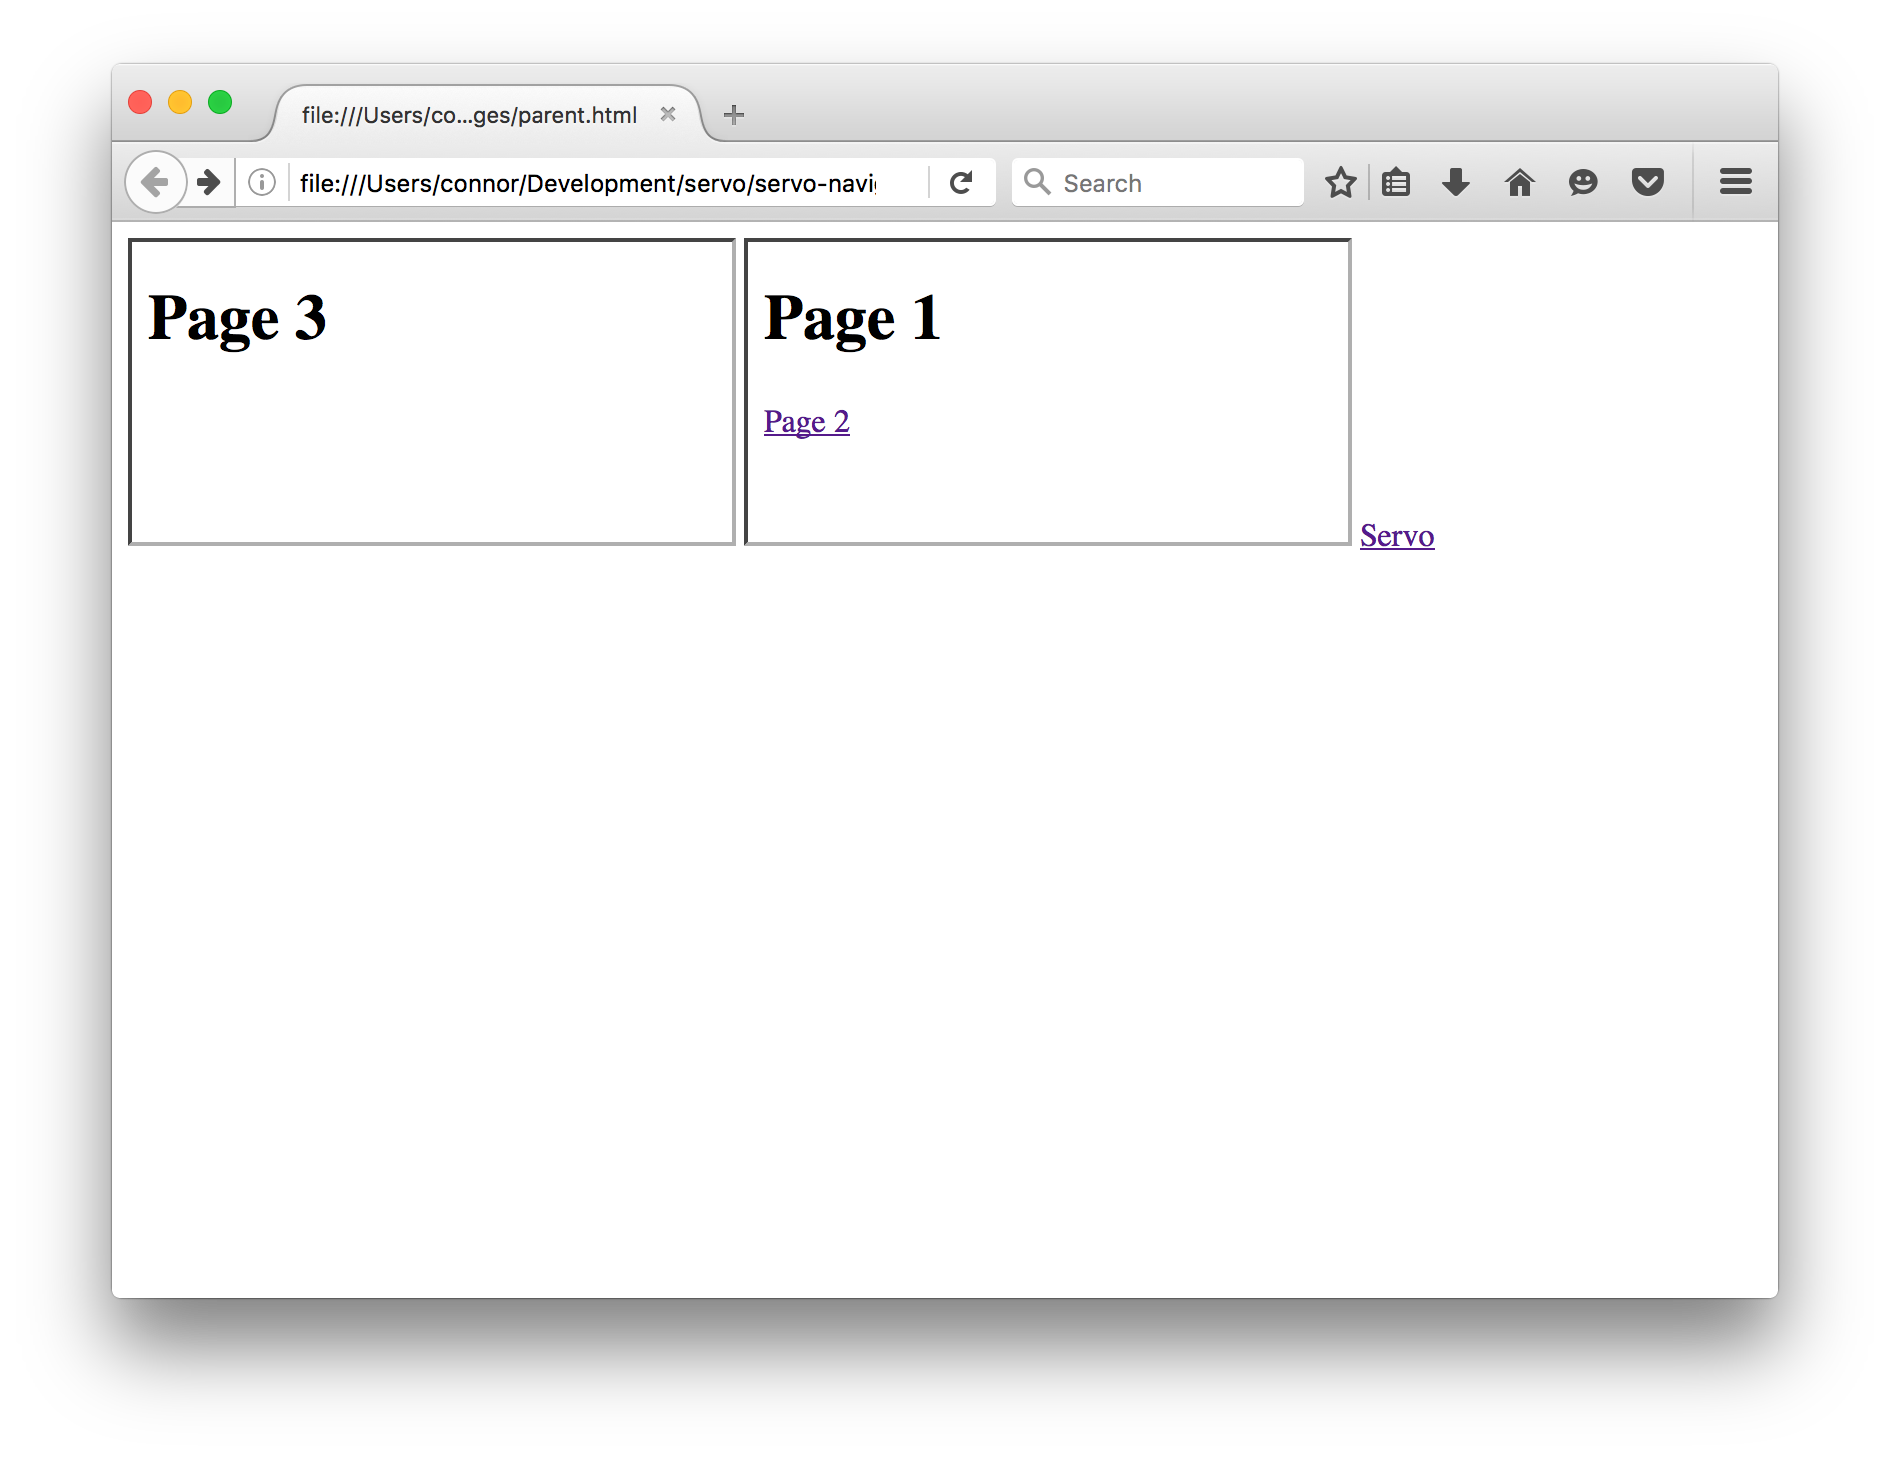
\includegraphics[width=.5\linewidth]{images/experiments/forwardback4/firefox/6.png}
    }~\raisebox{-.5\height}{
      \begin{tikzpicture}
        \node[doc,active,fully](0) at (0,0){0};
        \node[doc](1) at (1,-1){1};
        \node[doc,jshactive,fully](2) at (2,-2){2};
        \node[doc](3) at (3,-1){3};
        \node[doc,active,fully](4) at (4,-1){4};
        \node[doc](5) at (5,-2){5};
        \node[doc](6) at (6,-2){6};
        \node[draw,dotted,fit=(0)]{};
        \node[draw,dotted,fit=(1)(4)]{};
        \node[draw,dotted,fit=(2)(6)]{};
        \draw[->](0)to[out=0,in=140](4);
        \draw[->](0)to[out=-20,in=90](2);
      \end{tikzpicture}
    }
    \caption{Traversal by $-4$.}
    \label{fig:traverseback4}
  \end{figure}

  This state is obviously wrong, as document $4$ should have traversed to document $1$.
  This is similar to counterexample~\ref{counterexample:homomorphism1}.

  \emph{$\aNH'$ traverses the history by $4$ to $\aNH''$}:
  \begin{figure}[H]
    \raisebox{-.5\height}{
      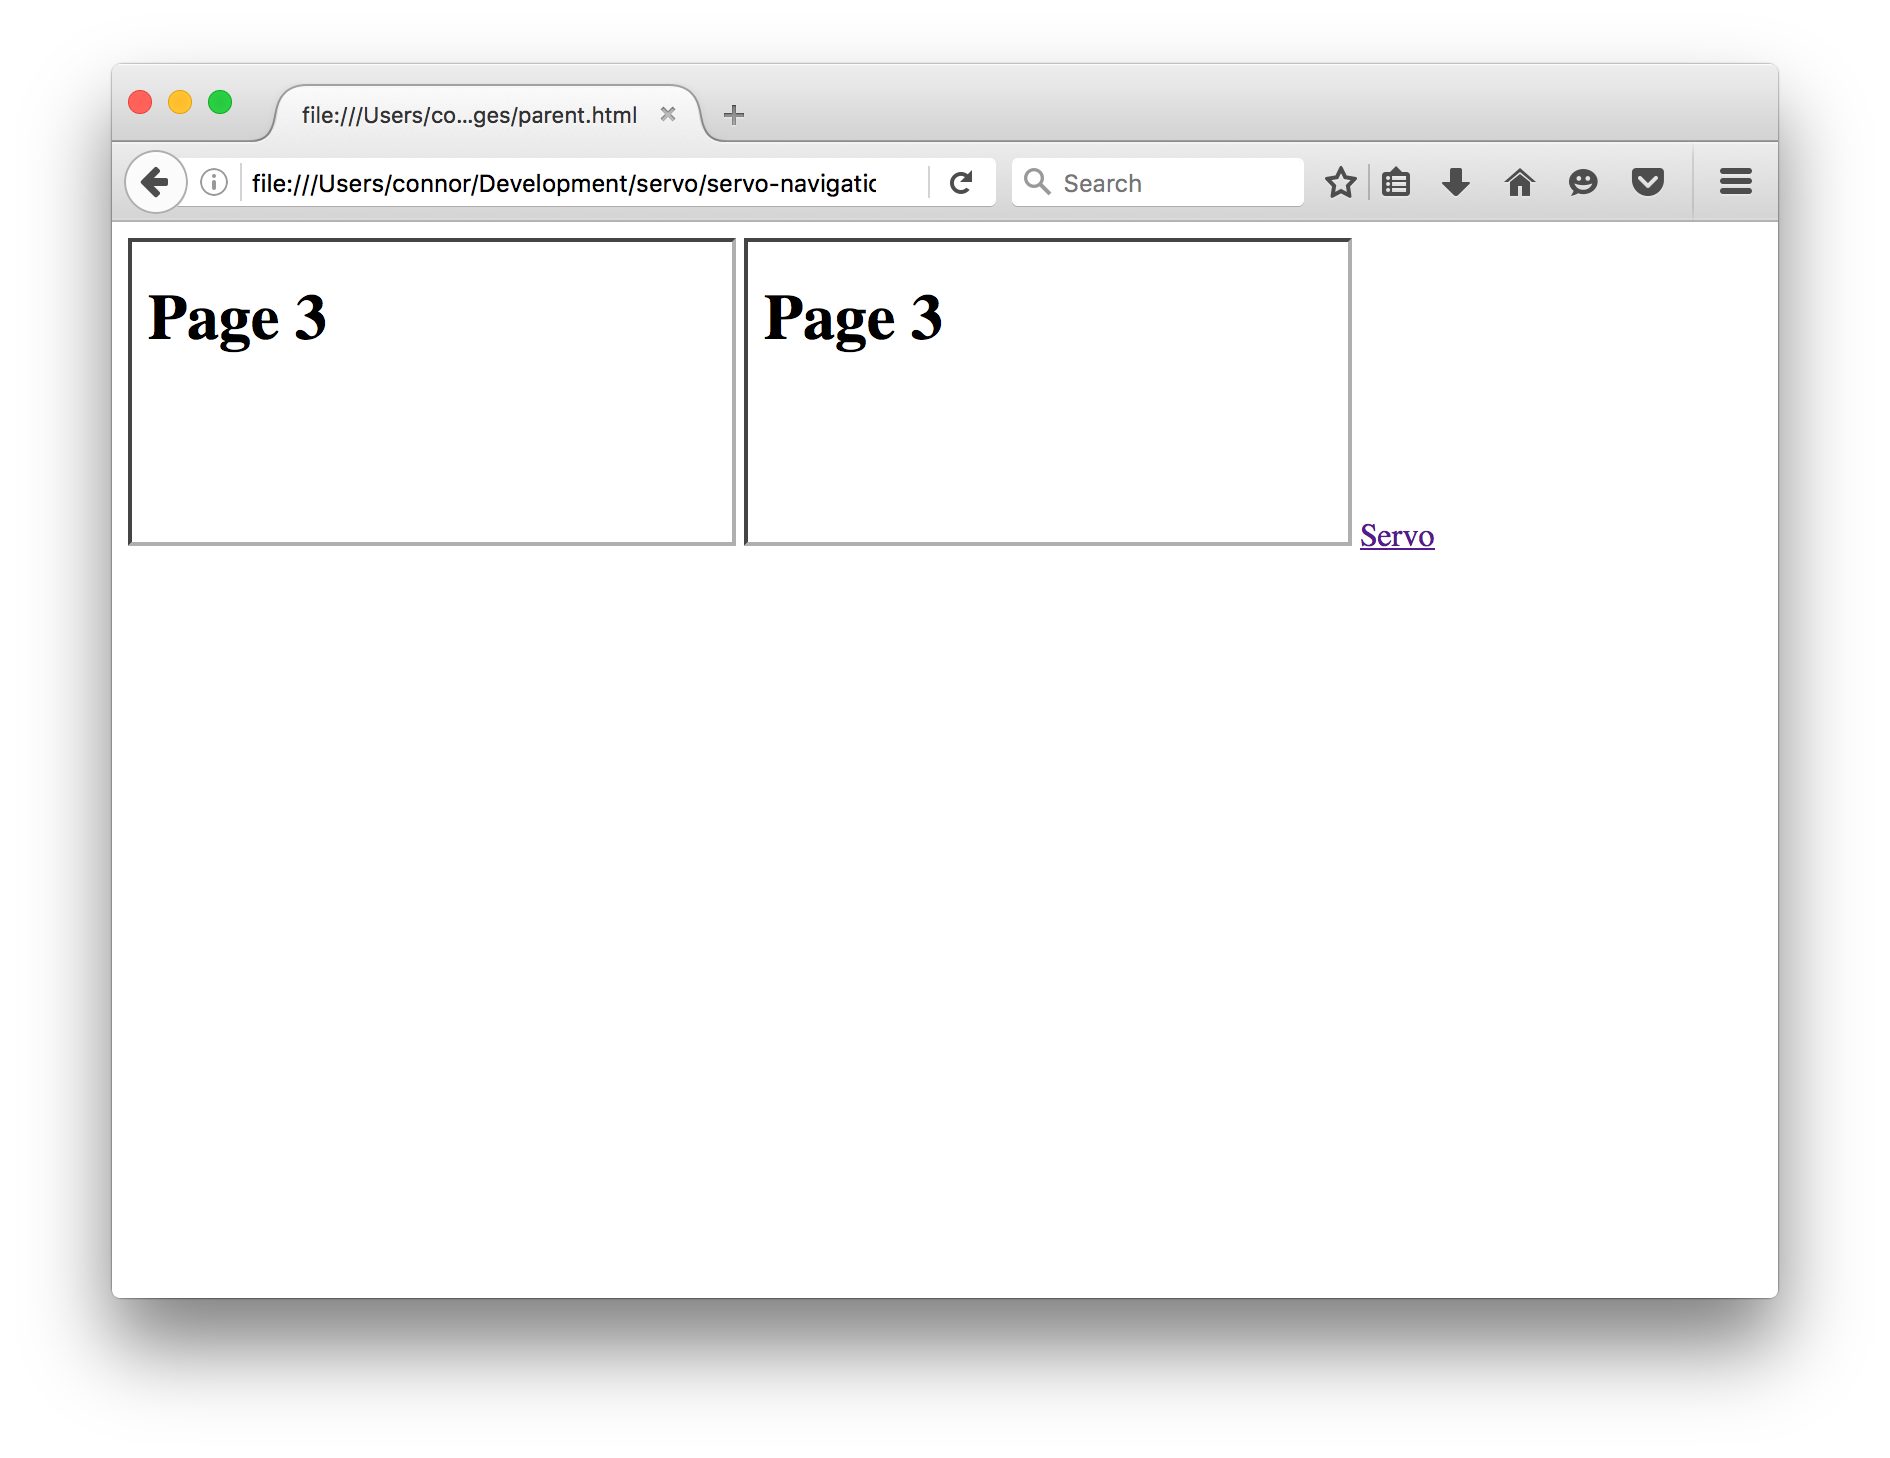
\includegraphics[width=.5\linewidth]{images/experiments/forwardback4/firefox/7.png}
    }~\raisebox{-.5\height}{
      \begin{tikzpicture}
        \node[doc,active,fully](0) at (0,0){0};
        \node[doc](1) at (1,-1){1};
        \node[doc](2) at (2,-2){2};
        \node[doc](3) at (3,-1){3};
        \node[doc,active,fully](4) at (4,-1){4};
        \node[doc](5) at (5,-2){5};
        \node[doc,jshactive,fully](6) at (6,-2){6};
        \node[draw,dotted,fit=(0)]{};
        \node[draw,dotted,fit=(1)(4)]{};
        \node[draw,dotted,fit=(2)(6)]{};
        \draw[->](0)to[out=0,in=140](4);
        \draw[->](0)to[out=0,in=120](6);
      \end{tikzpicture}
    }
    \caption{Traversal by $4$.}
  \end{figure}

  While this result does satisfy Goal~\ref{goal:homomorphism}, there are still some issues:
  \begin{itemize}
    \item Figure~\ref{fig:traverseback4} yields an incorrect traversal. [CGB: I believe this actually does break Goal~\ref{goal:homomorphism} as navigating by $-1$ four times should yield the correct state.]
    \item It is impossible to get back to Page 1 on both Frames. [CGB: Looks to be a bug in FF, when holding down the back button, the list of pages to traverse to shows up. Clicking on the oldest item on the list does nothing and does not activate that item.]
  \end{itemize}

  Safari:
  \begin{figure}[H]
    \raisebox{-.5\height}{
      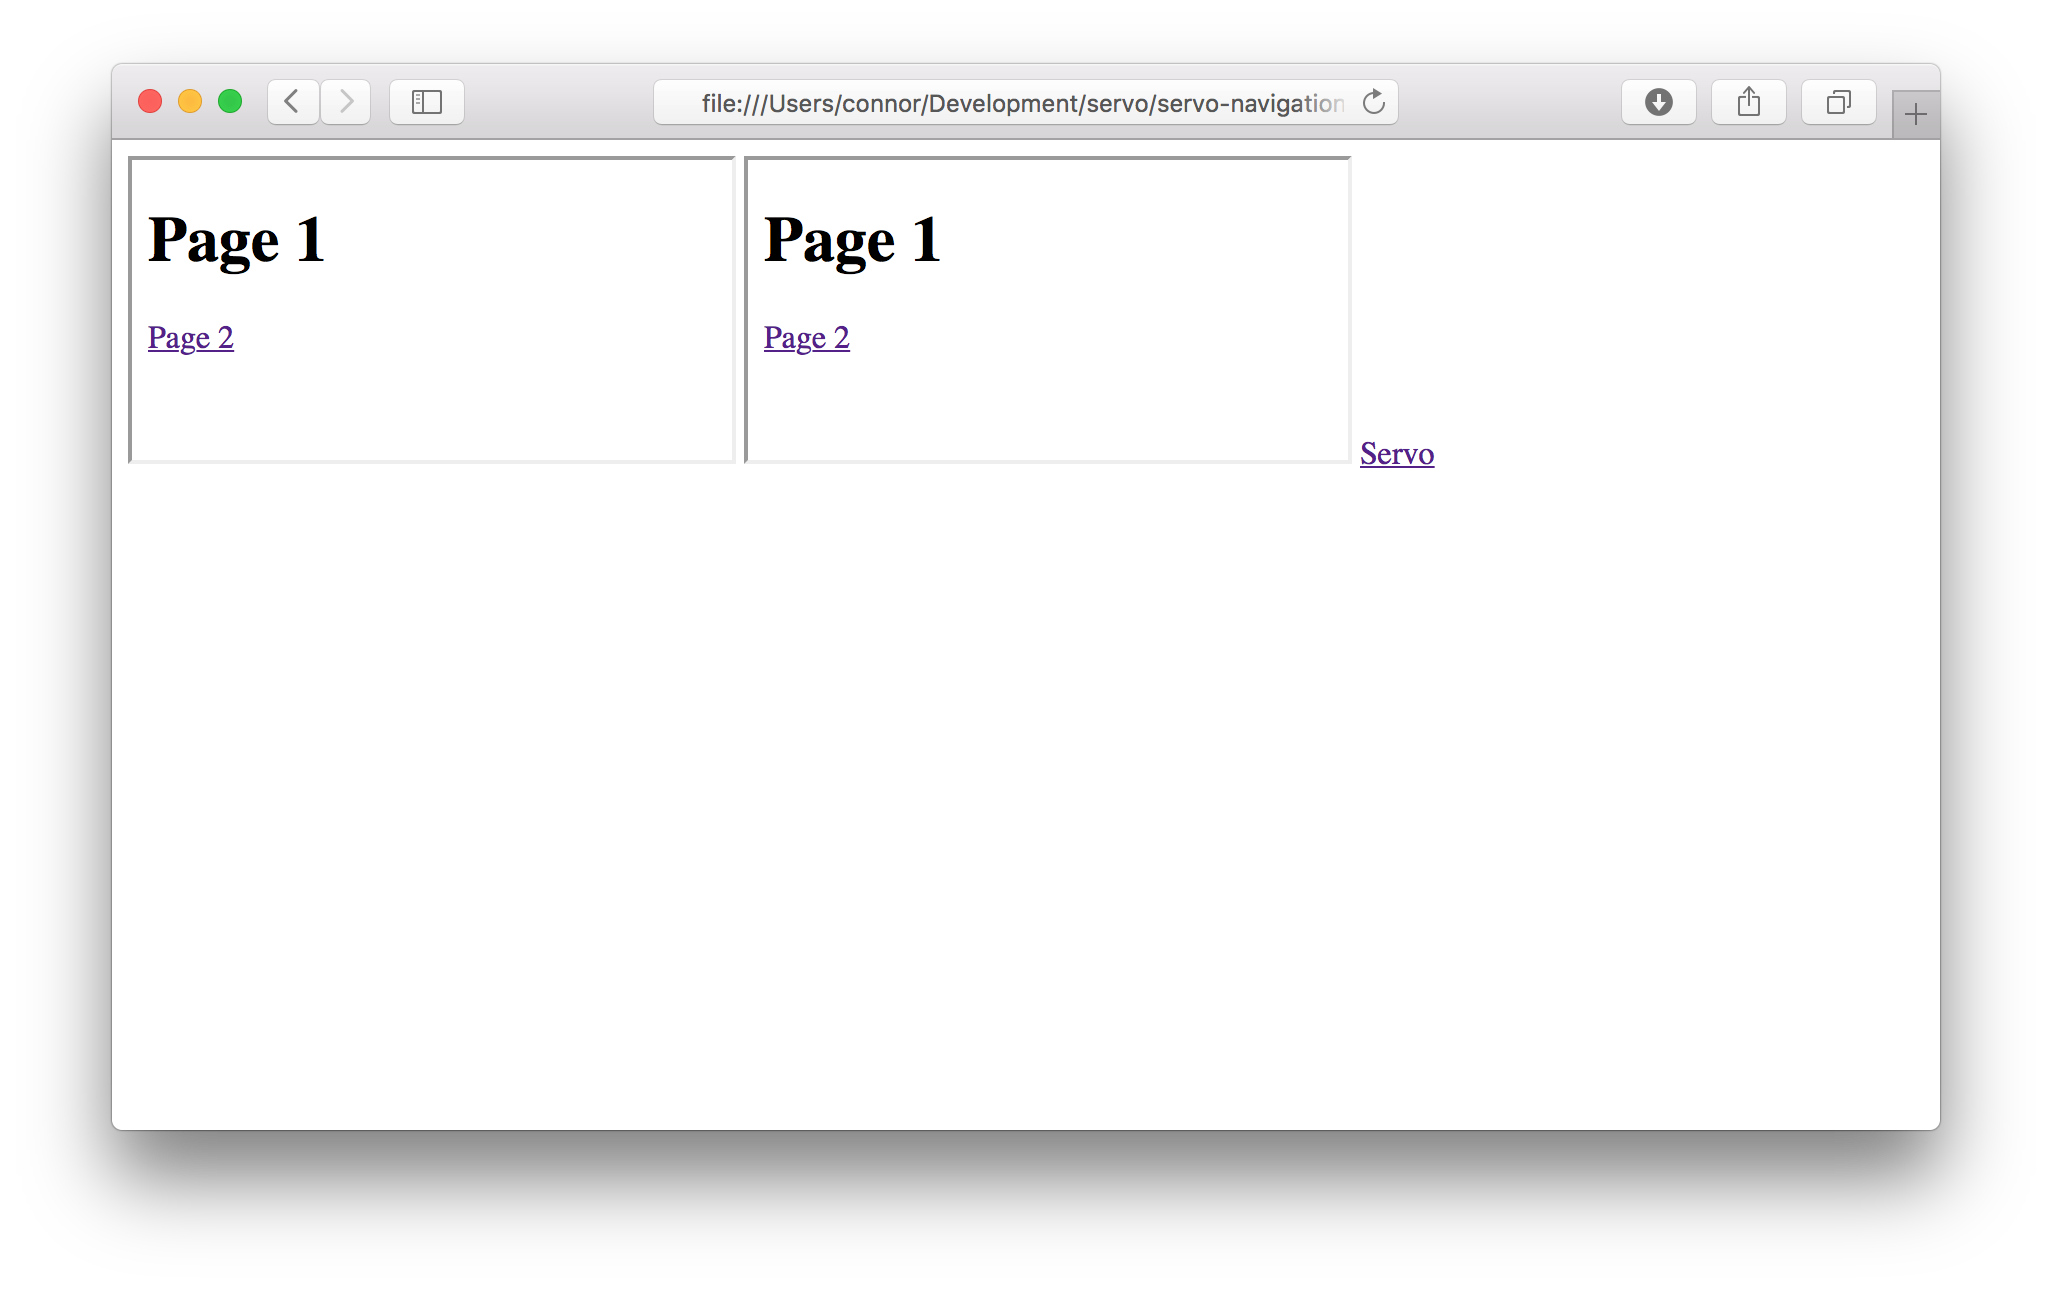
\includegraphics[width=.5\linewidth]{images/experiments/forwardback4/safari/1.png}%
    }~\raisebox{-.5\height}{
      \begin{tikzpicture}
        \node[doc,active,fully](0) at (0,0){0};
        \node[doc,active,fully](1) at (1,-1){1};
        \node[doc,jshactive,fully](2) at (2,-2){2};
        \node[draw,dotted,fit=(0)]{};
        \node[draw,dotted,fit=(1)]{};
        \node[draw,dotted,fit=(2)]{};
        \draw[->](0)--(1);
        \draw[->](0)to[out=-20,in=90](2);
      \end{tikzpicture}
    }
    \caption{Initial State}
  \end{figure}

  Navigate document $1$ to Page 2:
  \begin{figure}[H]
    \raisebox{-.5\height}{
      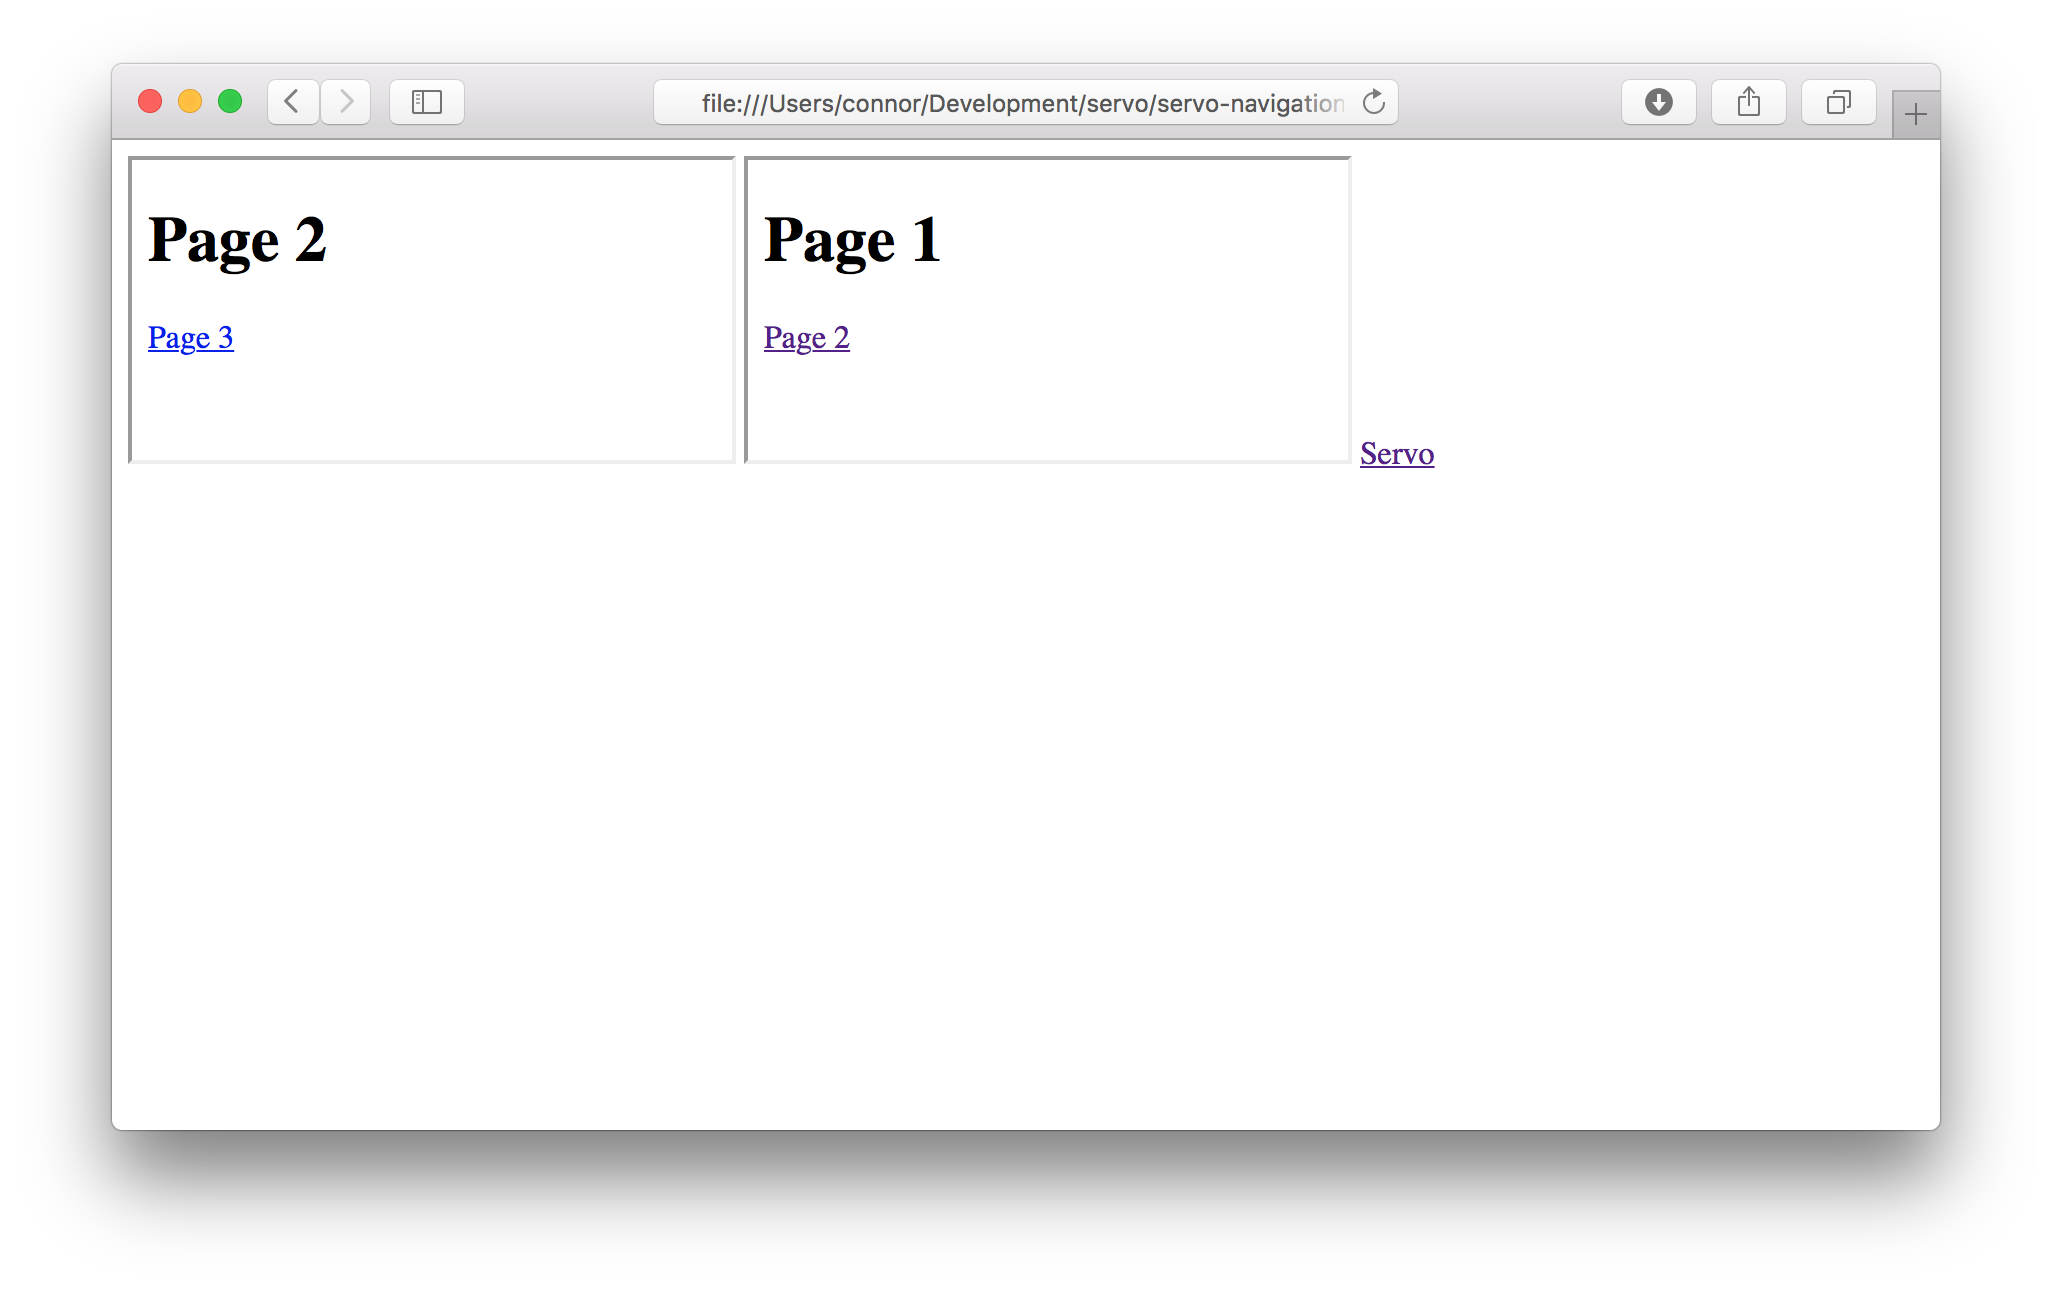
\includegraphics[width=.5\linewidth]{images/experiments/forwardback4/safari/2.png}
    }~\raisebox{-.5\height}{
      \begin{tikzpicture}
        \node[doc,active,fully](0) at (0,0){0};
        \node[doc](1) at (1,-1){1};
        \node[doc,active,fully](2) at (2,-2){2};
        \node[doc,jshactive,fully](3) at (3,-1){3};
        \node[draw,dotted,fit=(0)]{};
        \node[draw,dotted,fit=(1)(3)]{};
        \node[draw,dotted,fit=(2)]{};
        \draw[->](0)--(3);
        \draw[->](0)to[out=-20,in=90](2);
      \end{tikzpicture}
    }
    \caption{Navigate document $1$ to Page 2.}
  \end{figure}

  Navigate document $3$ to Page 3:
  \begin{figure}[H]
    \raisebox{-.5\height}{
      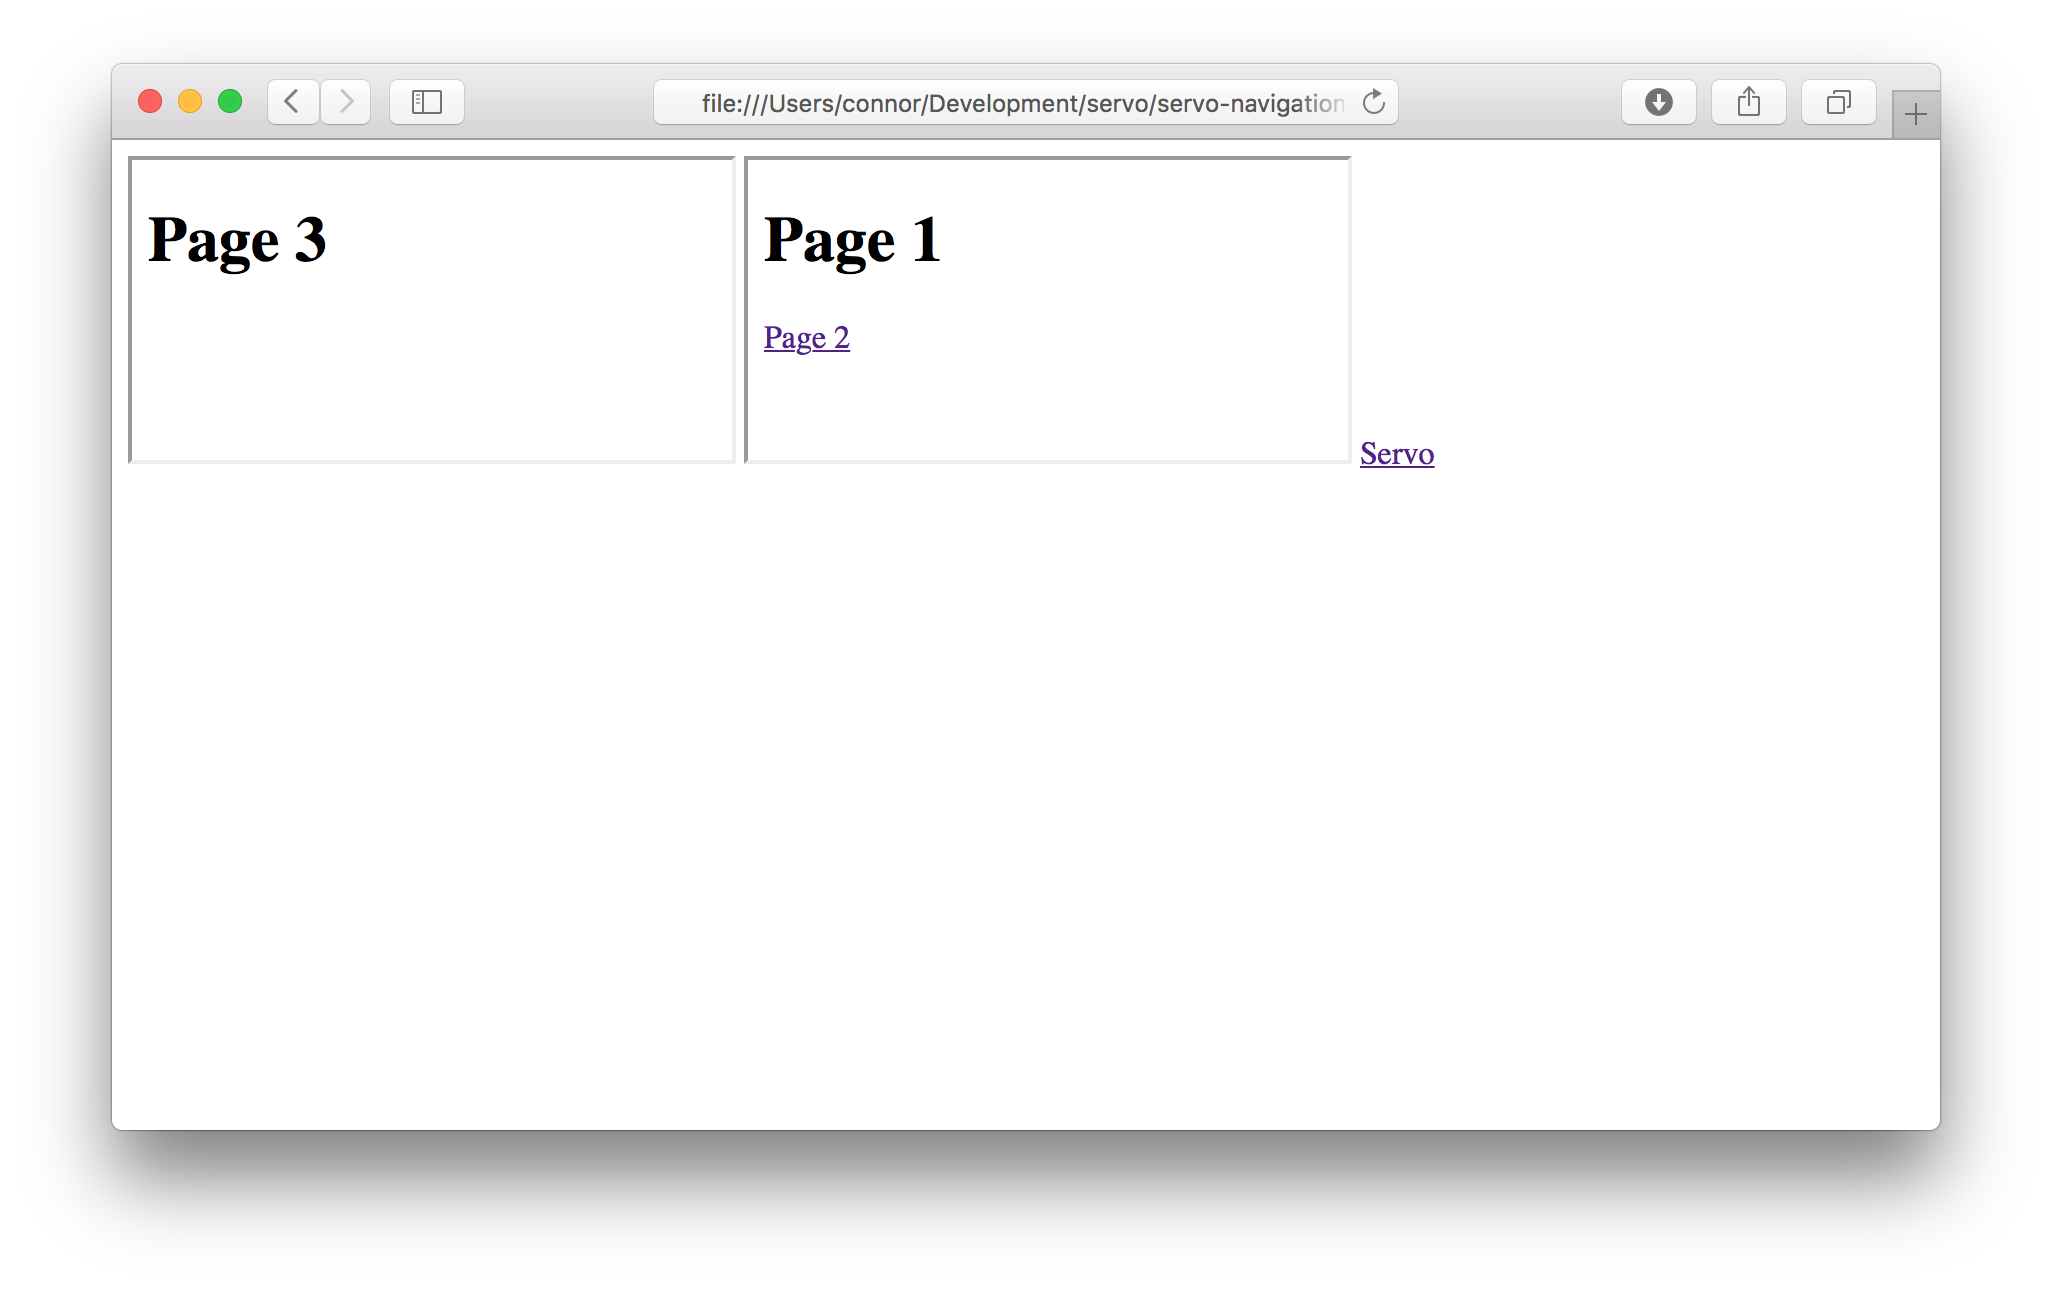
\includegraphics[width=.5\linewidth]{images/experiments/forwardback4/safari/3.png}
    }~\raisebox{-.5\height}{
      \begin{tikzpicture}
        \node[doc,active,fully](0) at (0,0){0};
        \node[doc](1) at (1,-1){1};
        \node[doc,active,fully](2) at (2,-2){2};
        \node[doc](3) at (3,-1){3};
        \node[doc,jshactive,fully](4) at (4,-1){4};
        \node[draw,dotted,fit=(0)]{};
        \node[draw,dotted,fit=(1)(4)]{};
        \node[draw,dotted,fit=(2)]{};
        \draw[->](0)to[out=0,in=140](4);
        \draw[->](0)to[out=-20,in=90](2);
      \end{tikzpicture}
    }
    \caption{Navigate document $3$ to Page 3.}
  \end{figure}

  Navigate document $2$ to Page 2:
  \begin{figure}[H]
    \raisebox{-.5\height}{
      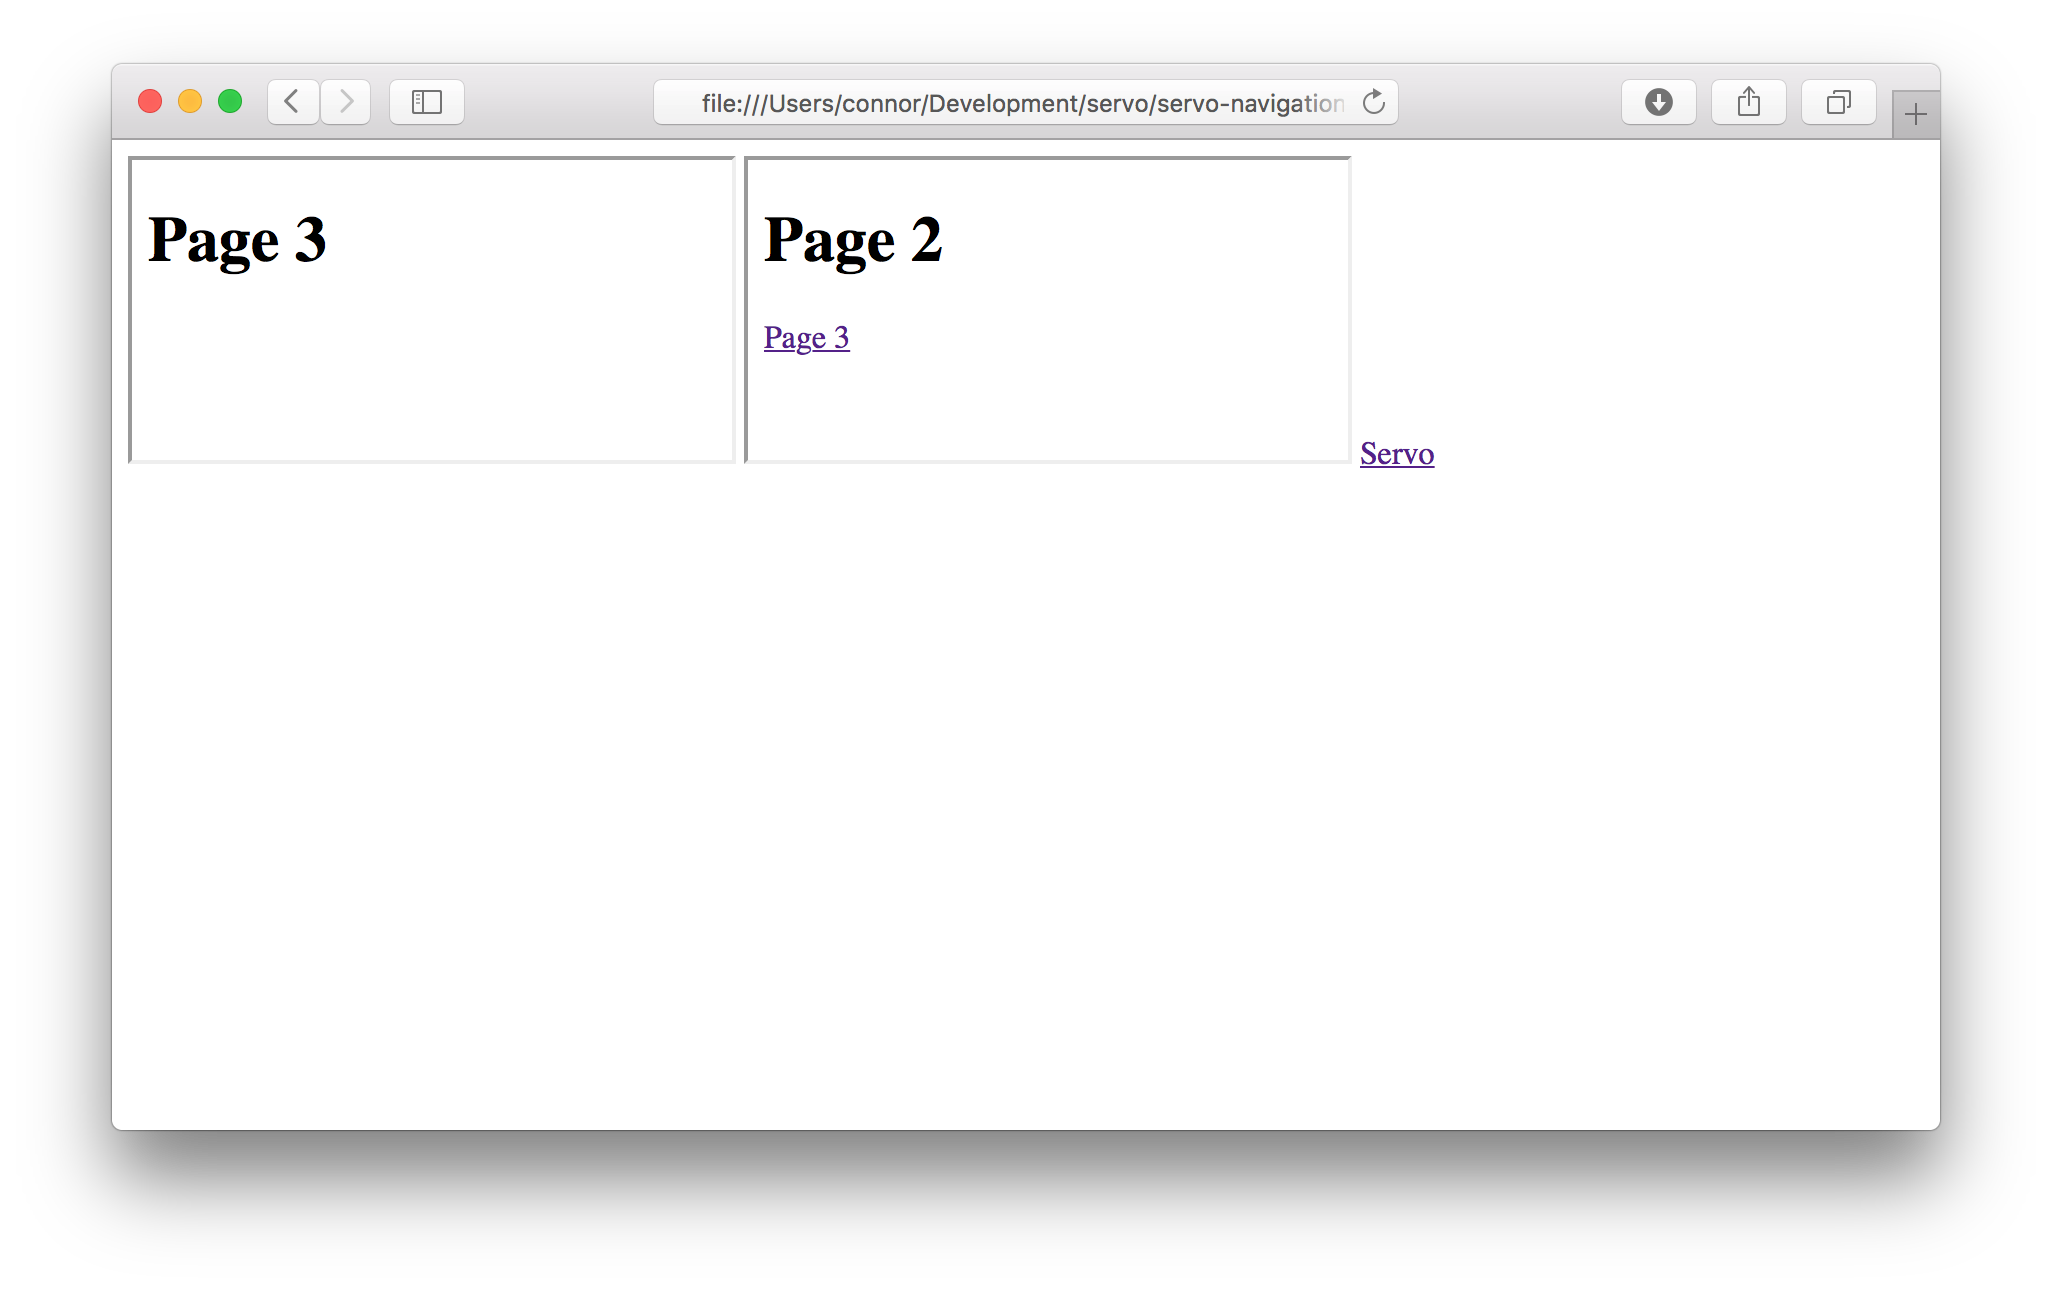
\includegraphics[width=.5\linewidth]{images/experiments/forwardback4/safari/4.png}
    }~\raisebox{-.5\height}{
      \begin{tikzpicture}
        \node[doc,active,fully](0) at (0,0){0};
        \node[doc](1) at (1,-1){1};
        \node[doc](2) at (2,-2){2};
        \node[doc](3) at (3,-1){3};
        \node[doc,active,fully](4) at (4,-1){4};
        \node[doc,jshactive,fully](5) at (5,-2){5};
        \node[draw,dotted,fit=(0)]{};
        \node[draw,dotted,fit=(1)(4)]{};
        \node[draw,dotted,fit=(2)(5)]{};
        \draw[->](0)to[out=0,in=140](4);
        \draw[->](0)to[out=0,in=90](5);
      \end{tikzpicture}
    }
    \caption{Navigate document $2$ to Page 2.}
  \end{figure}

  Navigate document $5$ to Page 3:
  \begin{figure}[H]
    \raisebox{-.5\height}{
      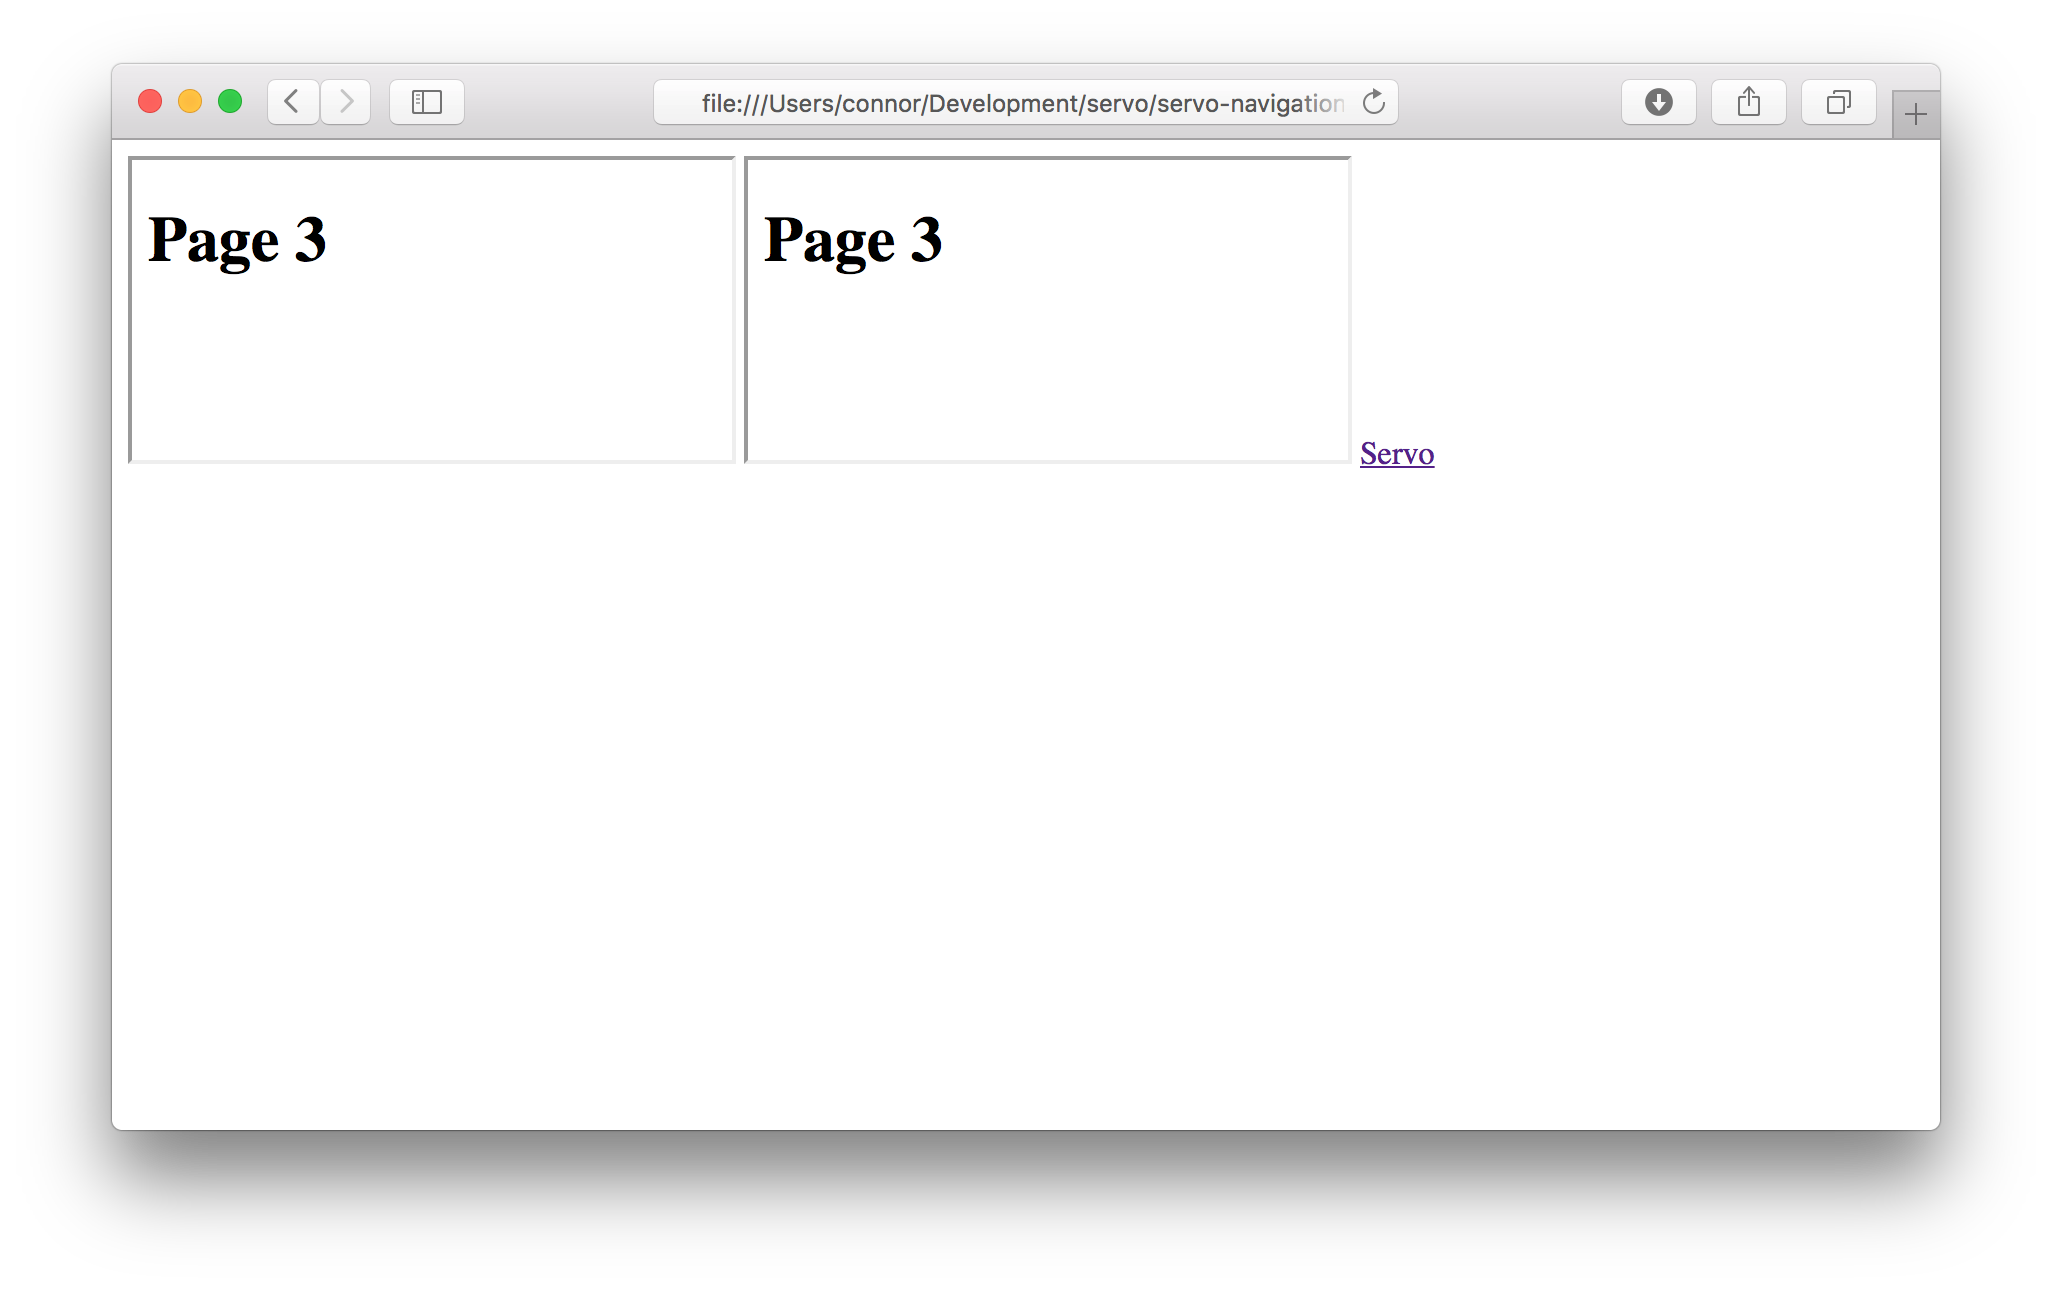
\includegraphics[width=.5\linewidth]{images/experiments/forwardback4/safari/5.png}
    }~\raisebox{-.5\height}{
      \begin{tikzpicture}
        \node[doc,active,fully](0) at (0,0){0};
        \node[doc](1) at (1,-1){1};
        \node[doc](2) at (2,-2){2};
        \node[doc](3) at (3,-1){3};
        \node[doc,active,fully](4) at (4,-1){4};
        \node[doc](5) at (5,-2){5};
        \node[doc,jshactive,fully](6) at (6,-2){6};
        \node[draw,dotted,fit=(0)]{};
        \node[draw,dotted,fit=(1)(4)]{};
        \node[draw,dotted,fit=(2)(6)]{};
        \draw[->](0)to[out=0,in=140](4);
        \draw[->](0)to[out=0,in=120](6);
      \end{tikzpicture}
    }
    \caption{Navigate document $5$ to Page 3.}
  \end{figure}

  \emph{$\aNH$ traverses the history by $-4$ to $\aNH'$}:
  \begin{figure}[H]
    \raisebox{-.5\height}{
      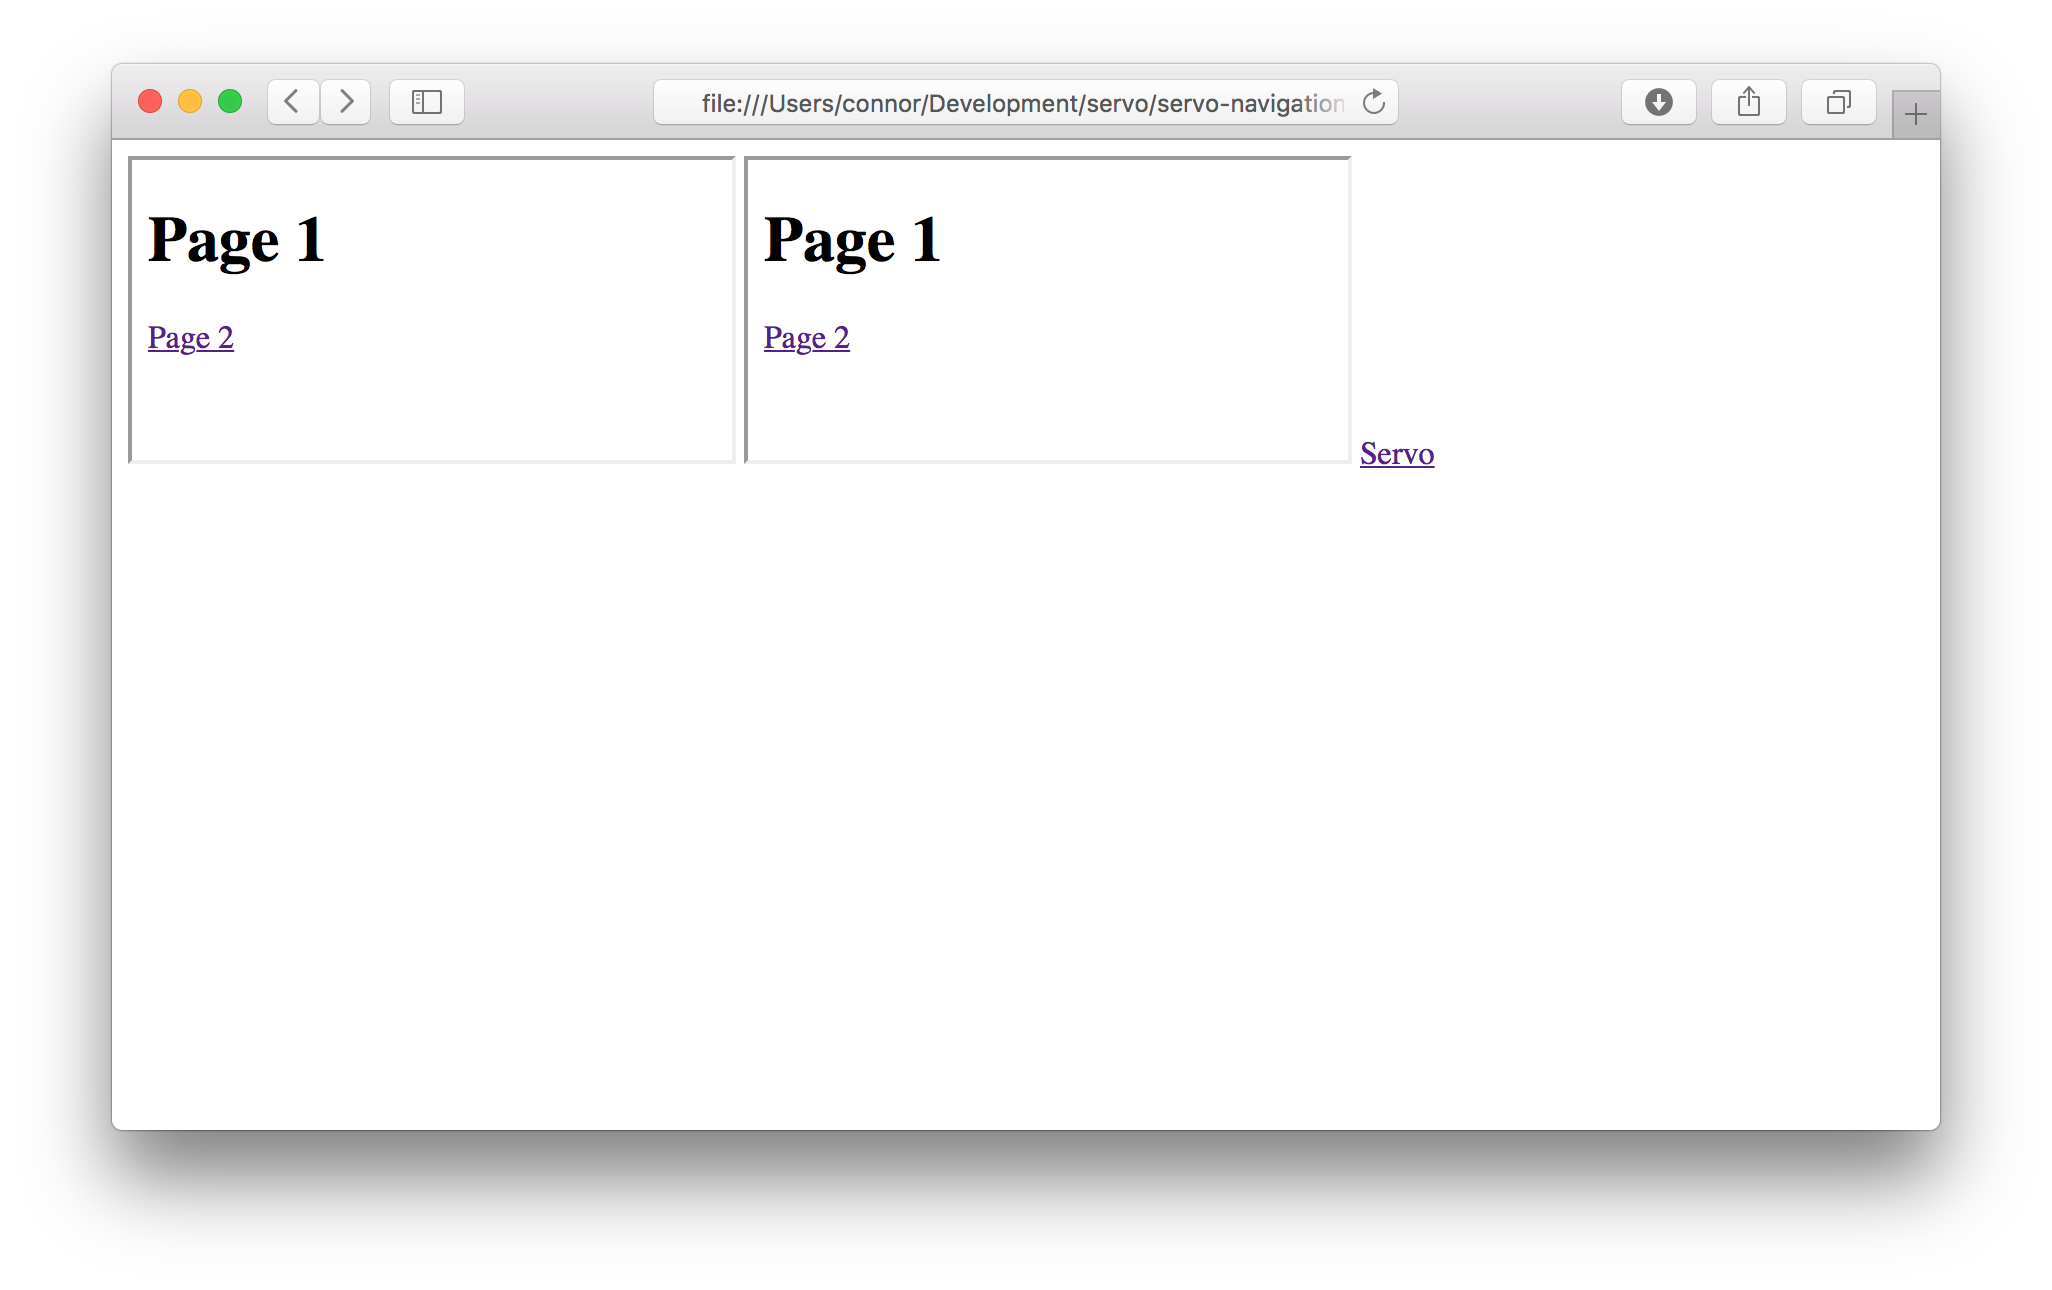
\includegraphics[width=.5\linewidth]{images/experiments/forwardback4/safari/6.png}
    }~\raisebox{-.5\height}{
      \begin{tikzpicture}
        \node[doc,active,fully](0) at (0,0){0};
        \node[doc,active,fully](1) at (1,-1){1};
        \node[doc,jshactive,fully](2) at (2,-2){2};
        \node[doc](3) at (3,-1){3};
        \node[doc](4) at (4,-1){4};
        \node[doc](5) at (5,-2){5};
        \node[doc](6) at (6,-2){6};
        \node[draw,dotted,fit=(0)]{};
        \node[draw,dotted,fit=(1)(4)]{};
        \node[draw,dotted,fit=(2)(6)]{};
        \draw[->](0)--(1);
        \draw[->](0)to[out=-20,in=90](2);
      \end{tikzpicture}
    }
    \caption{Traversal by $-4$.}
  \end{figure}

  \emph{$\aNH'$ traverses the history by $4$ to $\aNH''$}:
  \begin{figure}[H]
    \raisebox{-.5\height}{
      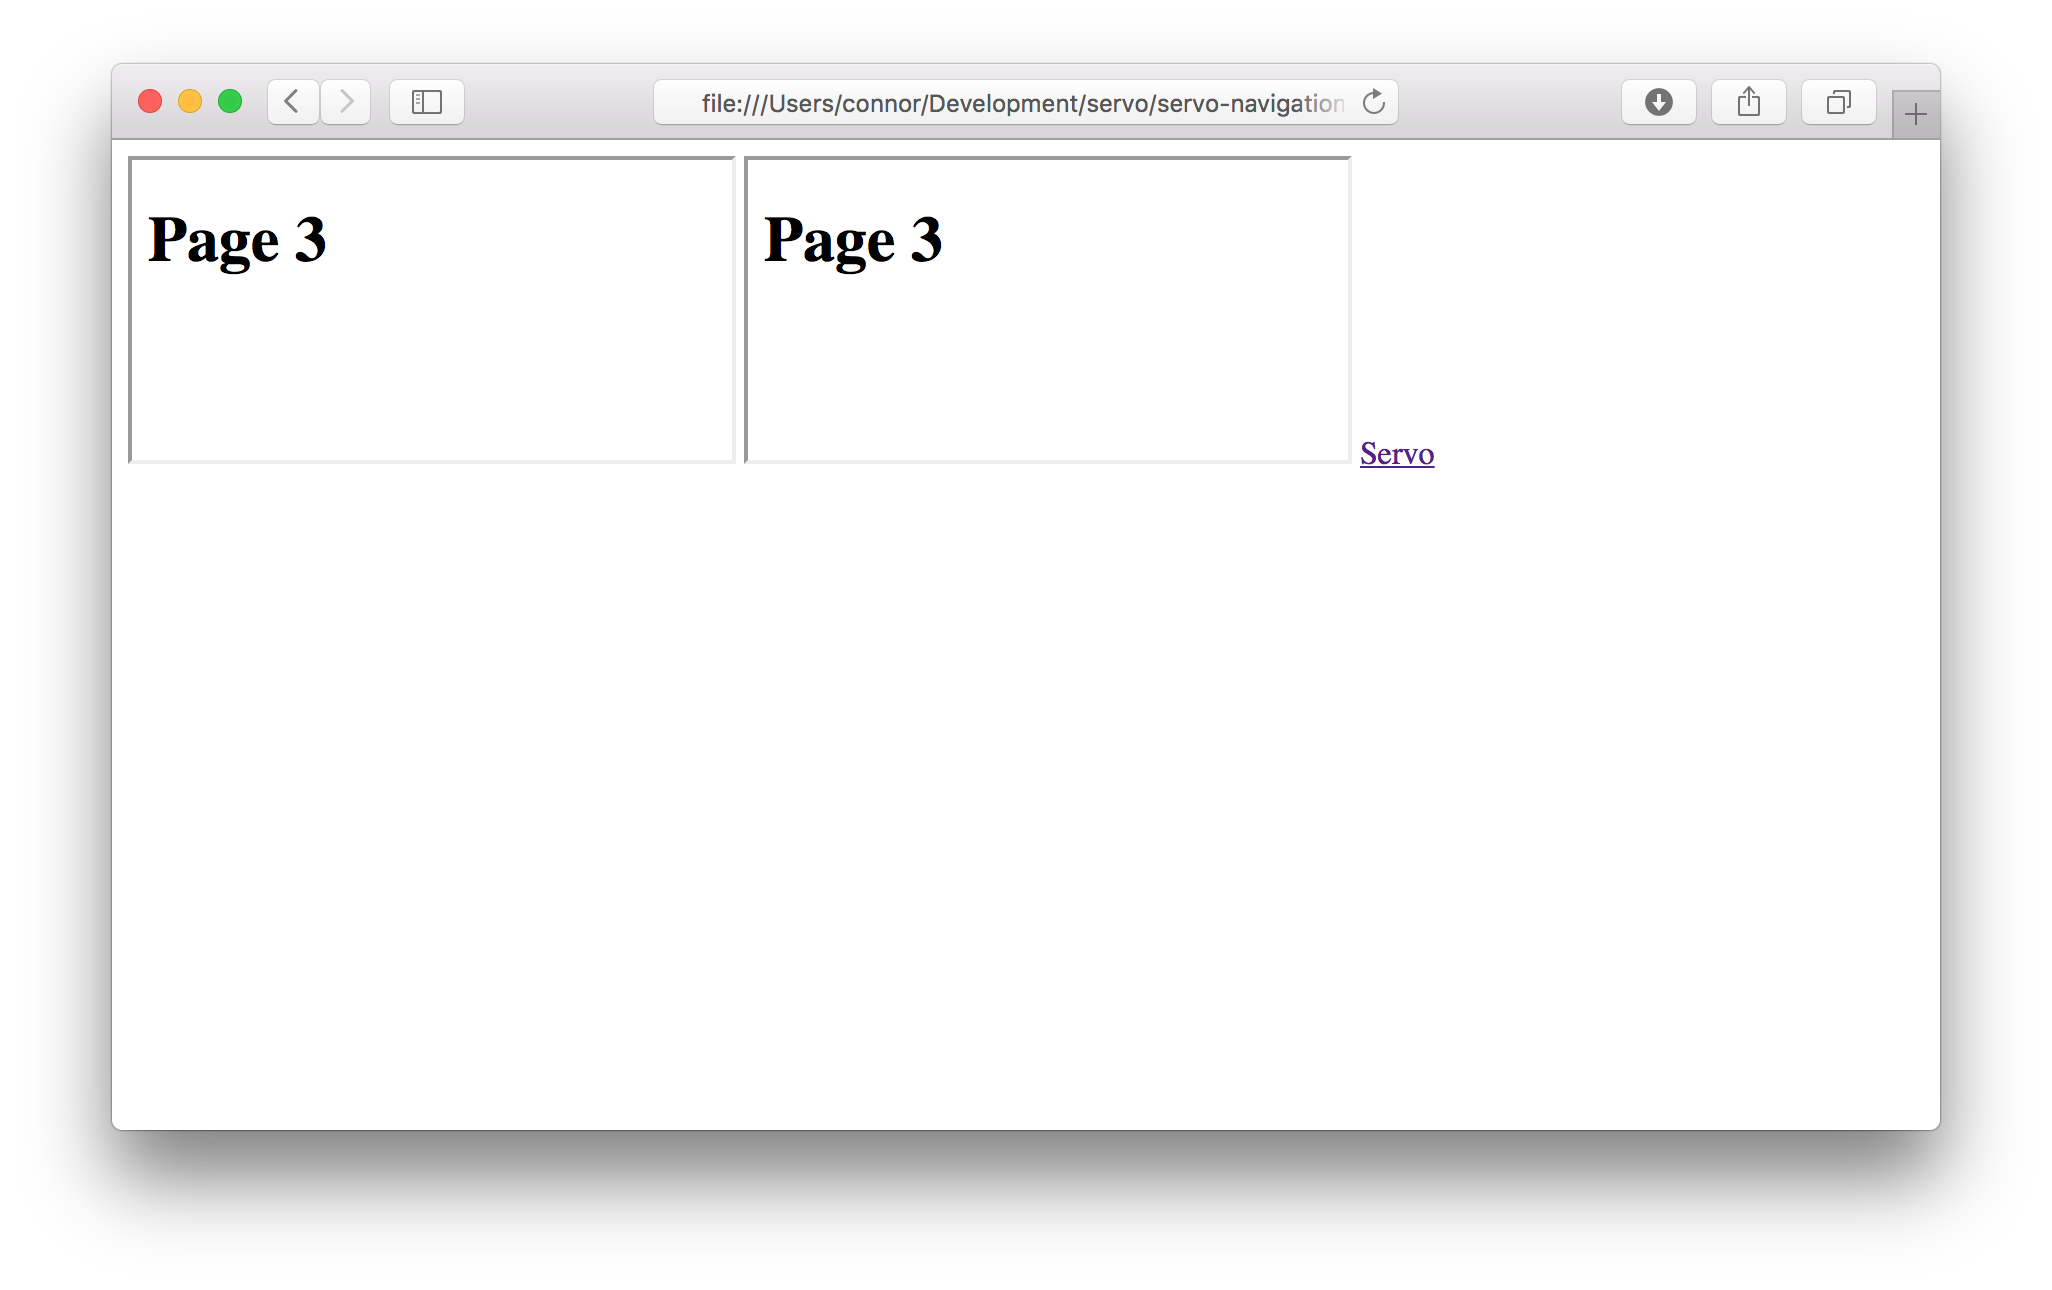
\includegraphics[width=.5\linewidth]{images/experiments/forwardback4/safari/7.png}
    }~\raisebox{-.5\height}{
      \begin{tikzpicture}
        \node[doc,active,fully](0) at (0,0){0};
        \node[doc](1) at (1,-1){1};
        \node[doc](2) at (2,-2){2};
        \node[doc](3) at (3,-1){3};
        \node[doc,active,fully](4) at (4,-1){4};
        \node[doc](5) at (5,-2){5};
        \node[doc,jshactive,fully](6) at (6,-2){6};
        \node[draw,dotted,fit=(0)]{};
        \node[draw,dotted,fit=(1)(4)]{};
        \node[draw,dotted,fit=(2)(6)]{};
        \draw[->](0)to[out=0,in=140](4);
        \draw[->](0)to[out=0,in=120](6);
      \end{tikzpicture}
    }
    \caption{Traversal by $4$.}
  \end{figure}

  These results in Safari satisfy Goal~\ref{goal:homomorphism}.

  Chrome:
  \begin{figure}[H]
    \raisebox{-.5\height}{
      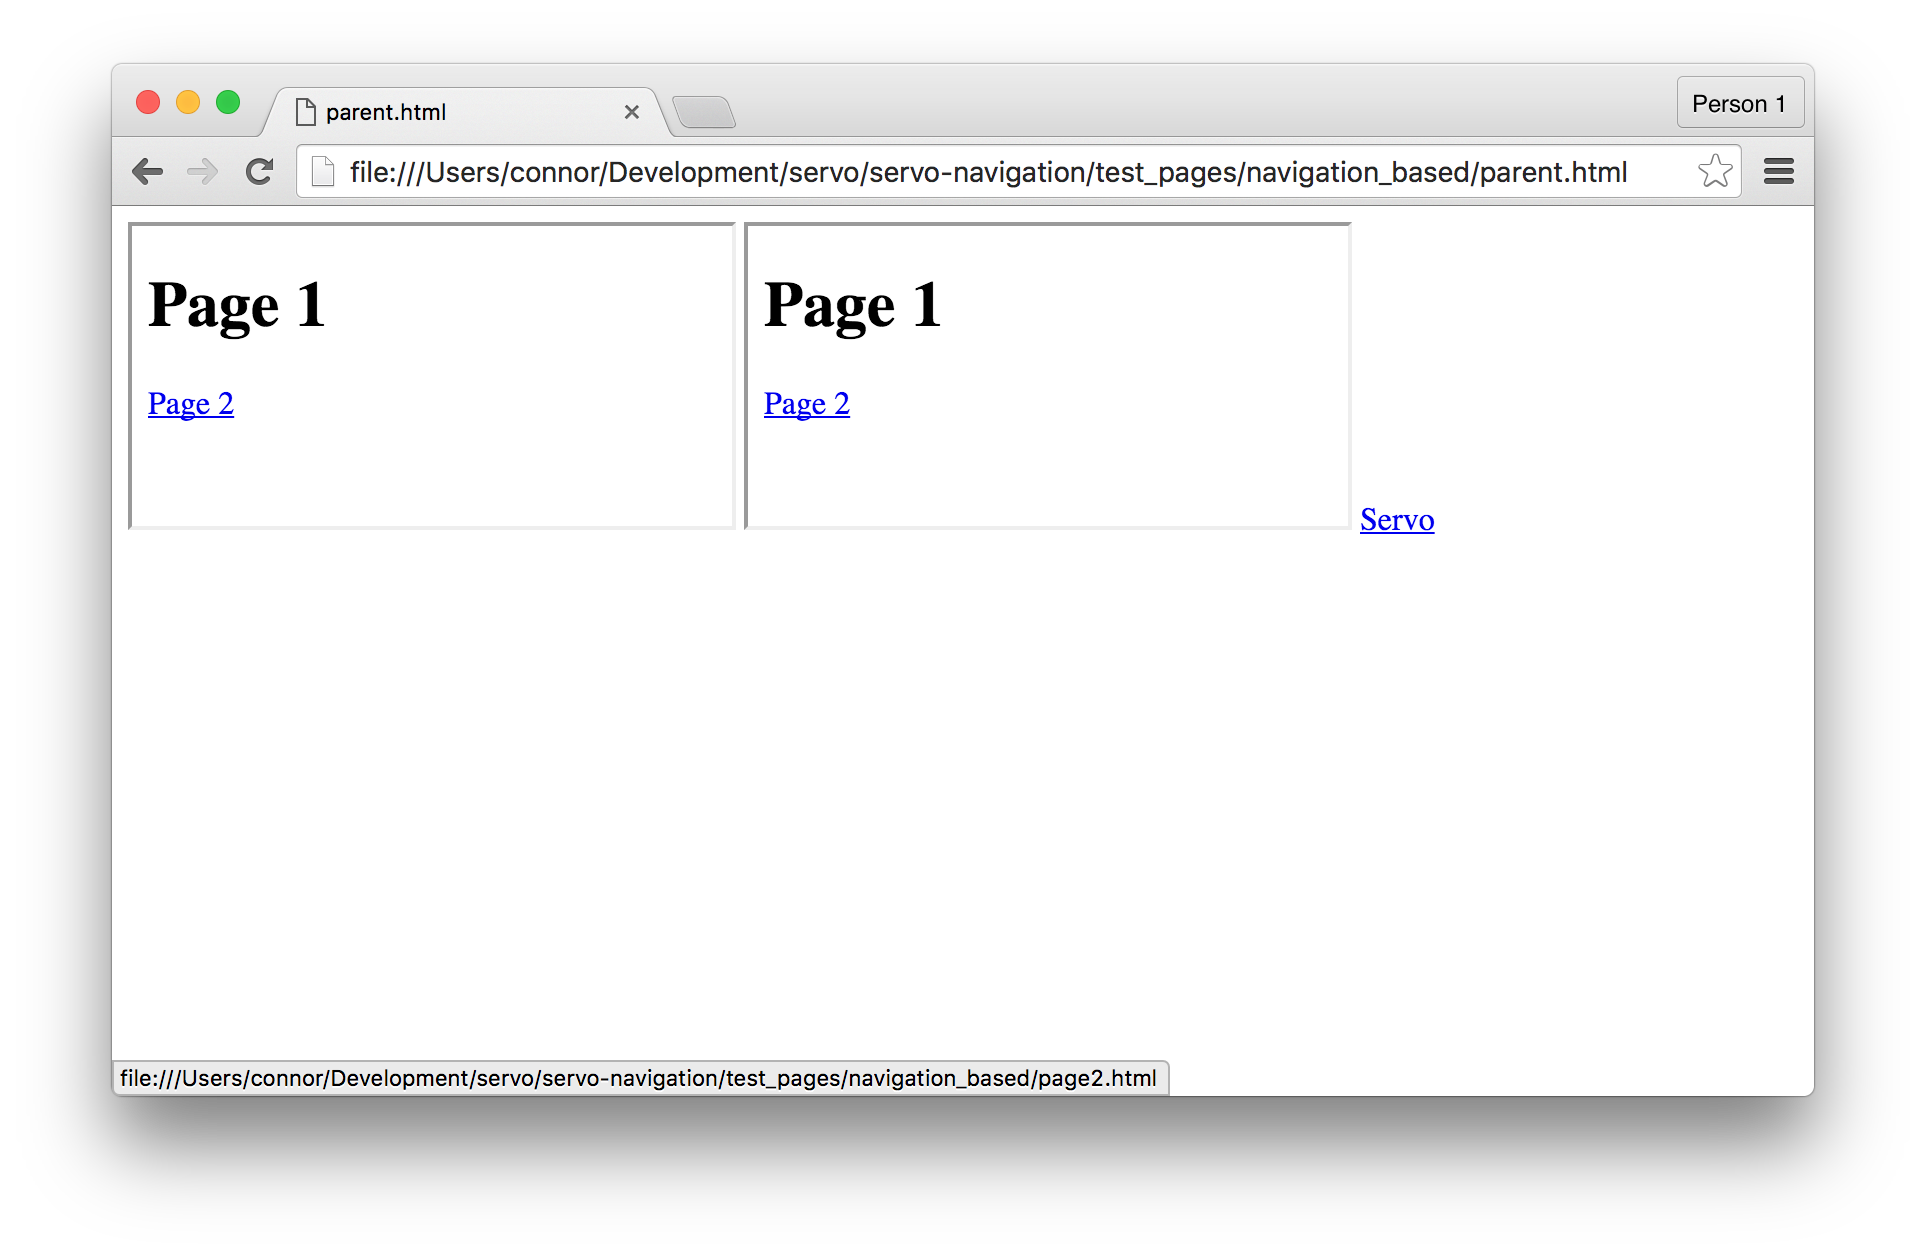
\includegraphics[width=.5\linewidth]{images/experiments/forwardback4/chrome/1.png}%
    }~\raisebox{-.5\height}{
      \begin{tikzpicture}
        \node[doc,active,fully](0) at (0,0){0};
        \node[doc,active,fully](1) at (1,-1){1};
        \node[doc,jshactive,fully](2) at (2,-2){2};
        \node[draw,dotted,fit=(0)]{};
        \node[draw,dotted,fit=(1)]{};
        \node[draw,dotted,fit=(2)]{};
        \draw[->](0)--(1);
        \draw[->](0)to[out=-20,in=90](2);
      \end{tikzpicture}
    }
    \caption{Initial State}
  \end{figure}

  Navigate document $1$ to Page 2:
  \begin{figure}[H]
    \raisebox{-.5\height}{
      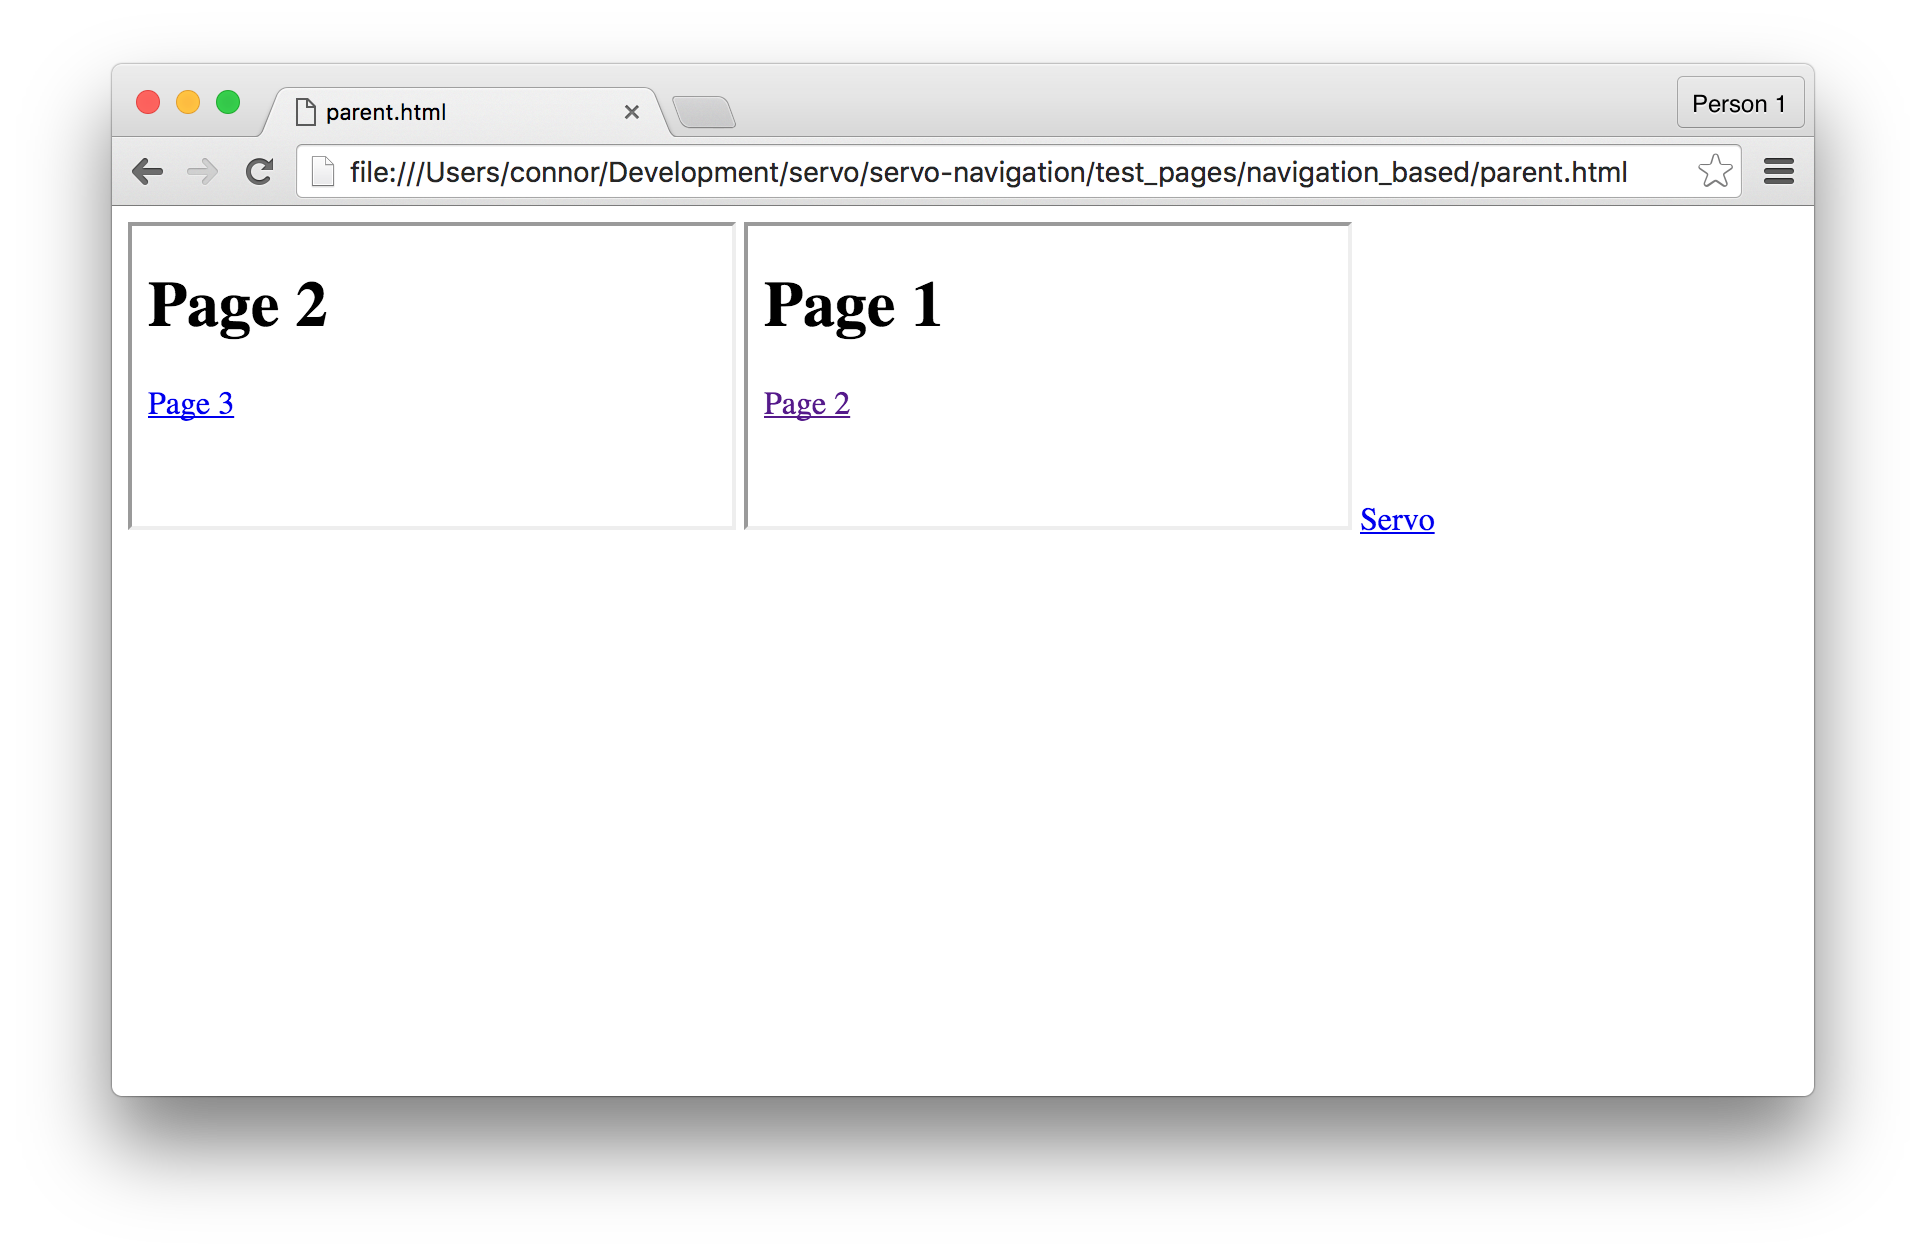
\includegraphics[width=.5\linewidth]{images/experiments/forwardback4/chrome/2.png}
    }~\raisebox{-.5\height}{
      \begin{tikzpicture}
        \node[doc,active,fully](0) at (0,0){0};
        \node[doc](1) at (1,-1){1};
        \node[doc,active,fully](2) at (2,-2){2};
        \node[doc,jshactive,fully](3) at (3,-1){3};
        \node[draw,dotted,fit=(0)]{};
        \node[draw,dotted,fit=(1)(3)]{};
        \node[draw,dotted,fit=(2)]{};
        \draw[->](0)--(3);
        \draw[->](0)to[out=-20,in=90](2);
      \end{tikzpicture}
    }
    \caption{Navigate document $1$ to Page 2.}
  \end{figure}

  Navigate document $3$ to Page 3:
  \begin{figure}[H]
    \raisebox{-.5\height}{
      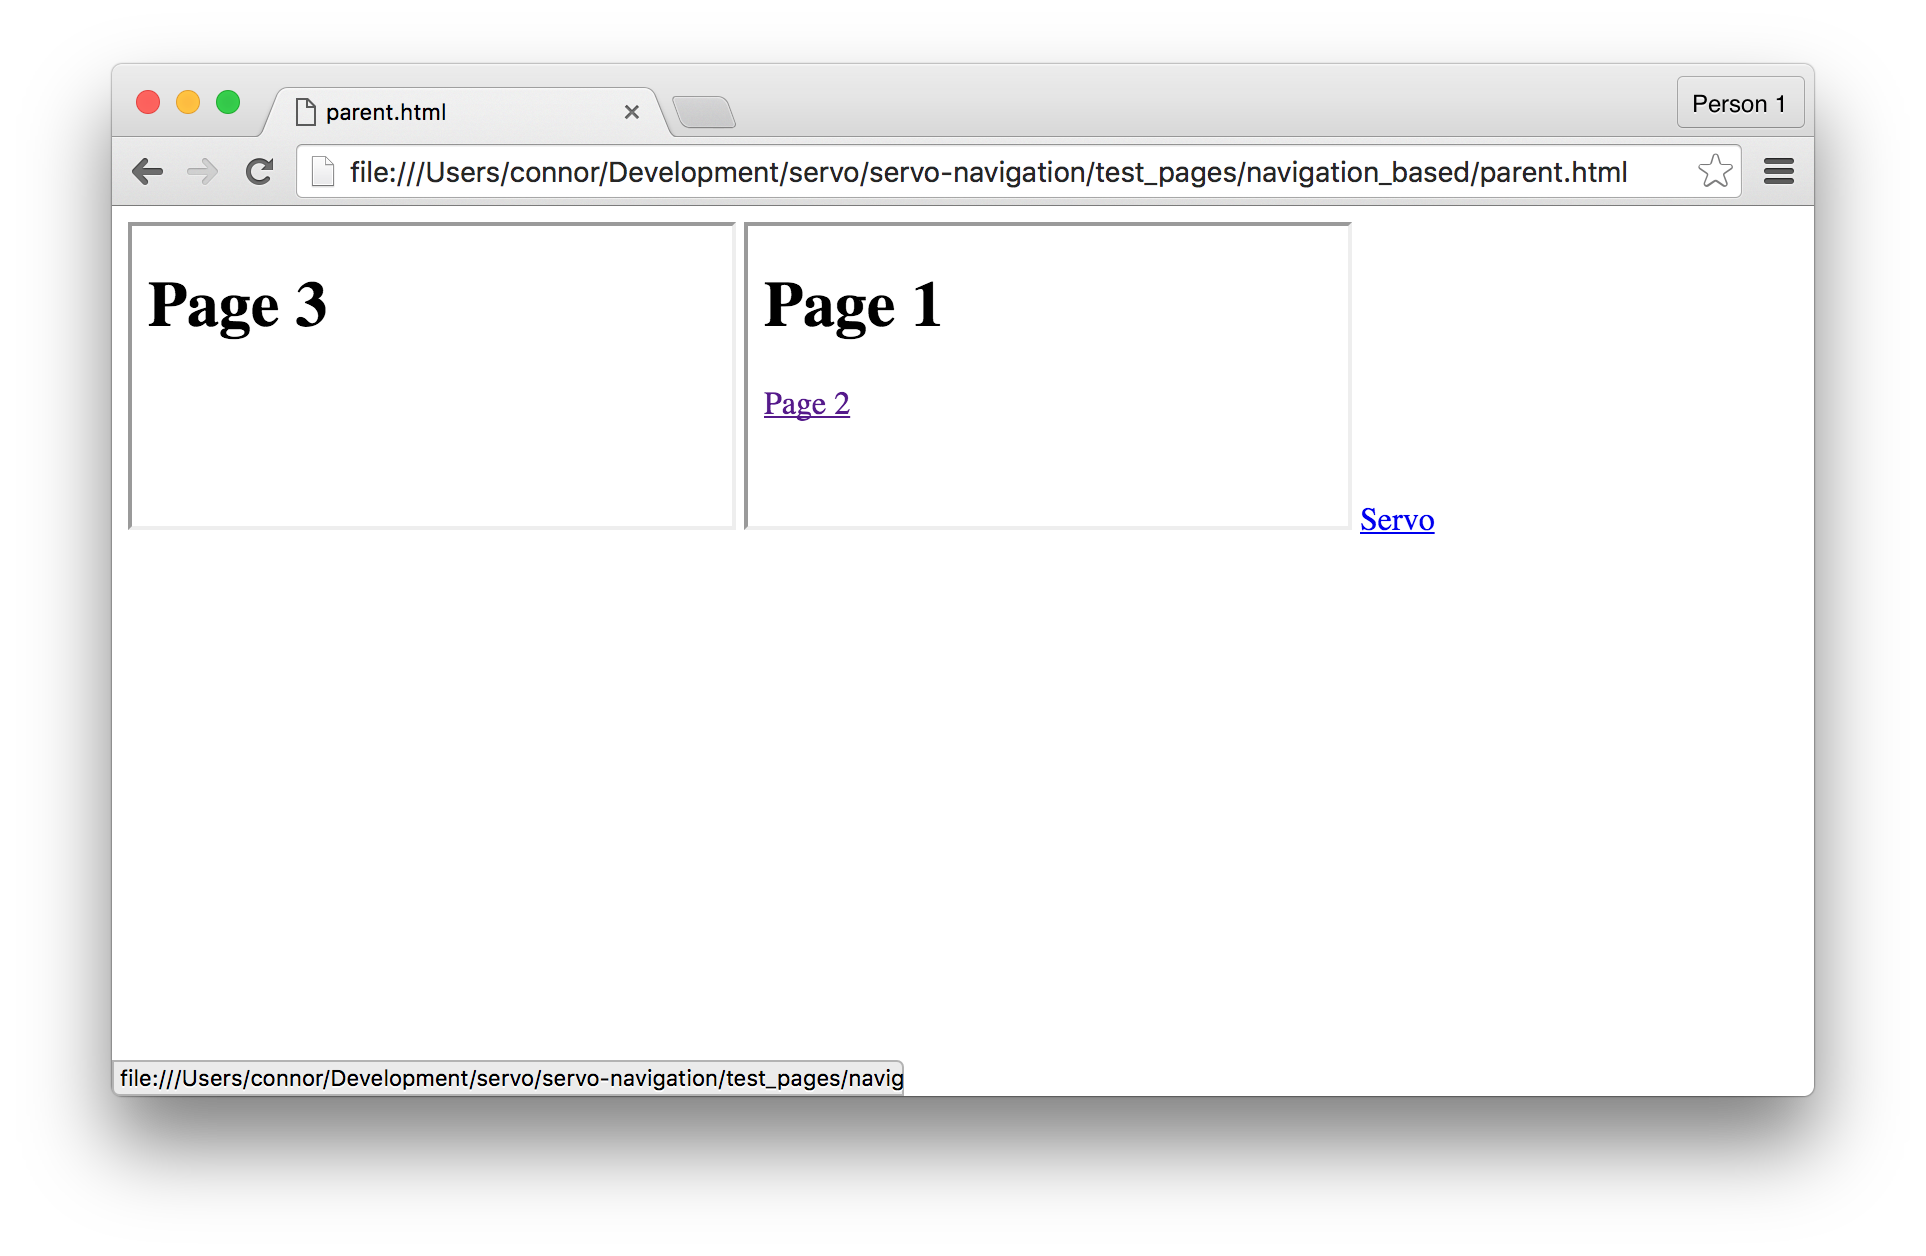
\includegraphics[width=.5\linewidth]{images/experiments/forwardback4/chrome/3.png}
    }~\raisebox{-.5\height}{
      \begin{tikzpicture}
        \node[doc,active,fully](0) at (0,0){0};
        \node[doc](1) at (1,-1){1};
        \node[doc,active,fully](2) at (2,-2){2};
        \node[doc](3) at (3,-1){3};
        \node[doc,jshactive,fully](4) at (4,-1){4};
        \node[draw,dotted,fit=(0)]{};
        \node[draw,dotted,fit=(1)(4)]{};
        \node[draw,dotted,fit=(2)]{};
        \draw[->](0)to[out=0,in=140](4);
        \draw[->](0)to[out=-20,in=90](2);
      \end{tikzpicture}
    }
    \caption{Navigate document $3$ to Page 3.}
  \end{figure}

  Navigate document $2$ to Page 2:
  \begin{figure}[H]
    \raisebox{-.5\height}{
      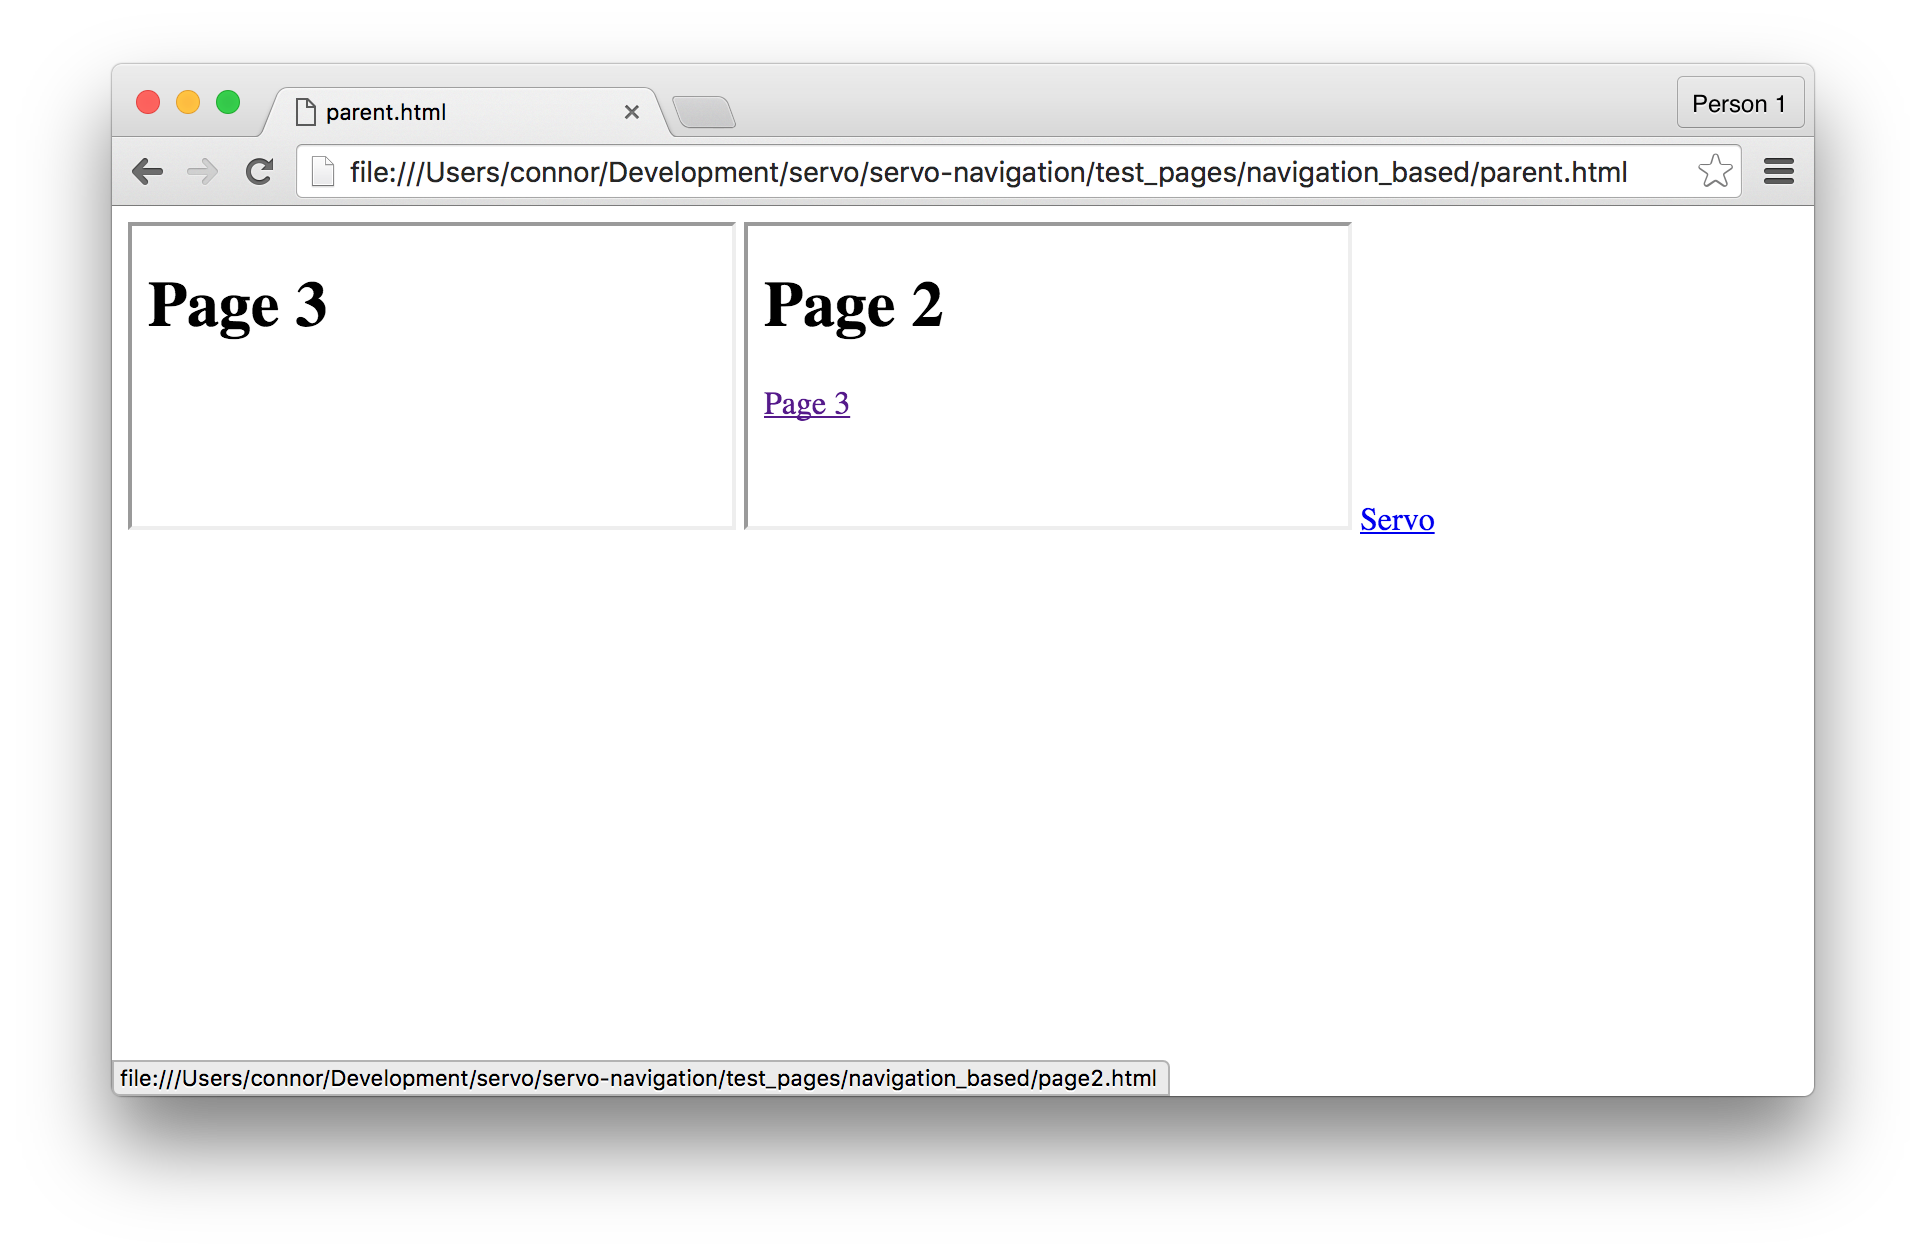
\includegraphics[width=.5\linewidth]{images/experiments/forwardback4/chrome/4.png}
    }~\raisebox{-.5\height}{
      \begin{tikzpicture}
        \node[doc,active,fully](0) at (0,0){0};
        \node[doc](1) at (1,-1){1};
        \node[doc](2) at (2,-2){2};
        \node[doc](3) at (3,-1){3};
        \node[doc,active,fully](4) at (4,-1){4};
        \node[doc,jshactive,fully](5) at (5,-2){5};
        \node[draw,dotted,fit=(0)]{};
        \node[draw,dotted,fit=(1)(4)]{};
        \node[draw,dotted,fit=(2)(5)]{};
        \draw[->](0)to[out=0,in=140](4);
        \draw[->](0)to[out=0,in=90](5);
      \end{tikzpicture}
    }
    \caption{Navigate document $2$ to Page 2.}
  \end{figure}

  Navigate document $5$ to Page 3:
  \begin{figure}[H]
    \raisebox{-.5\height}{
      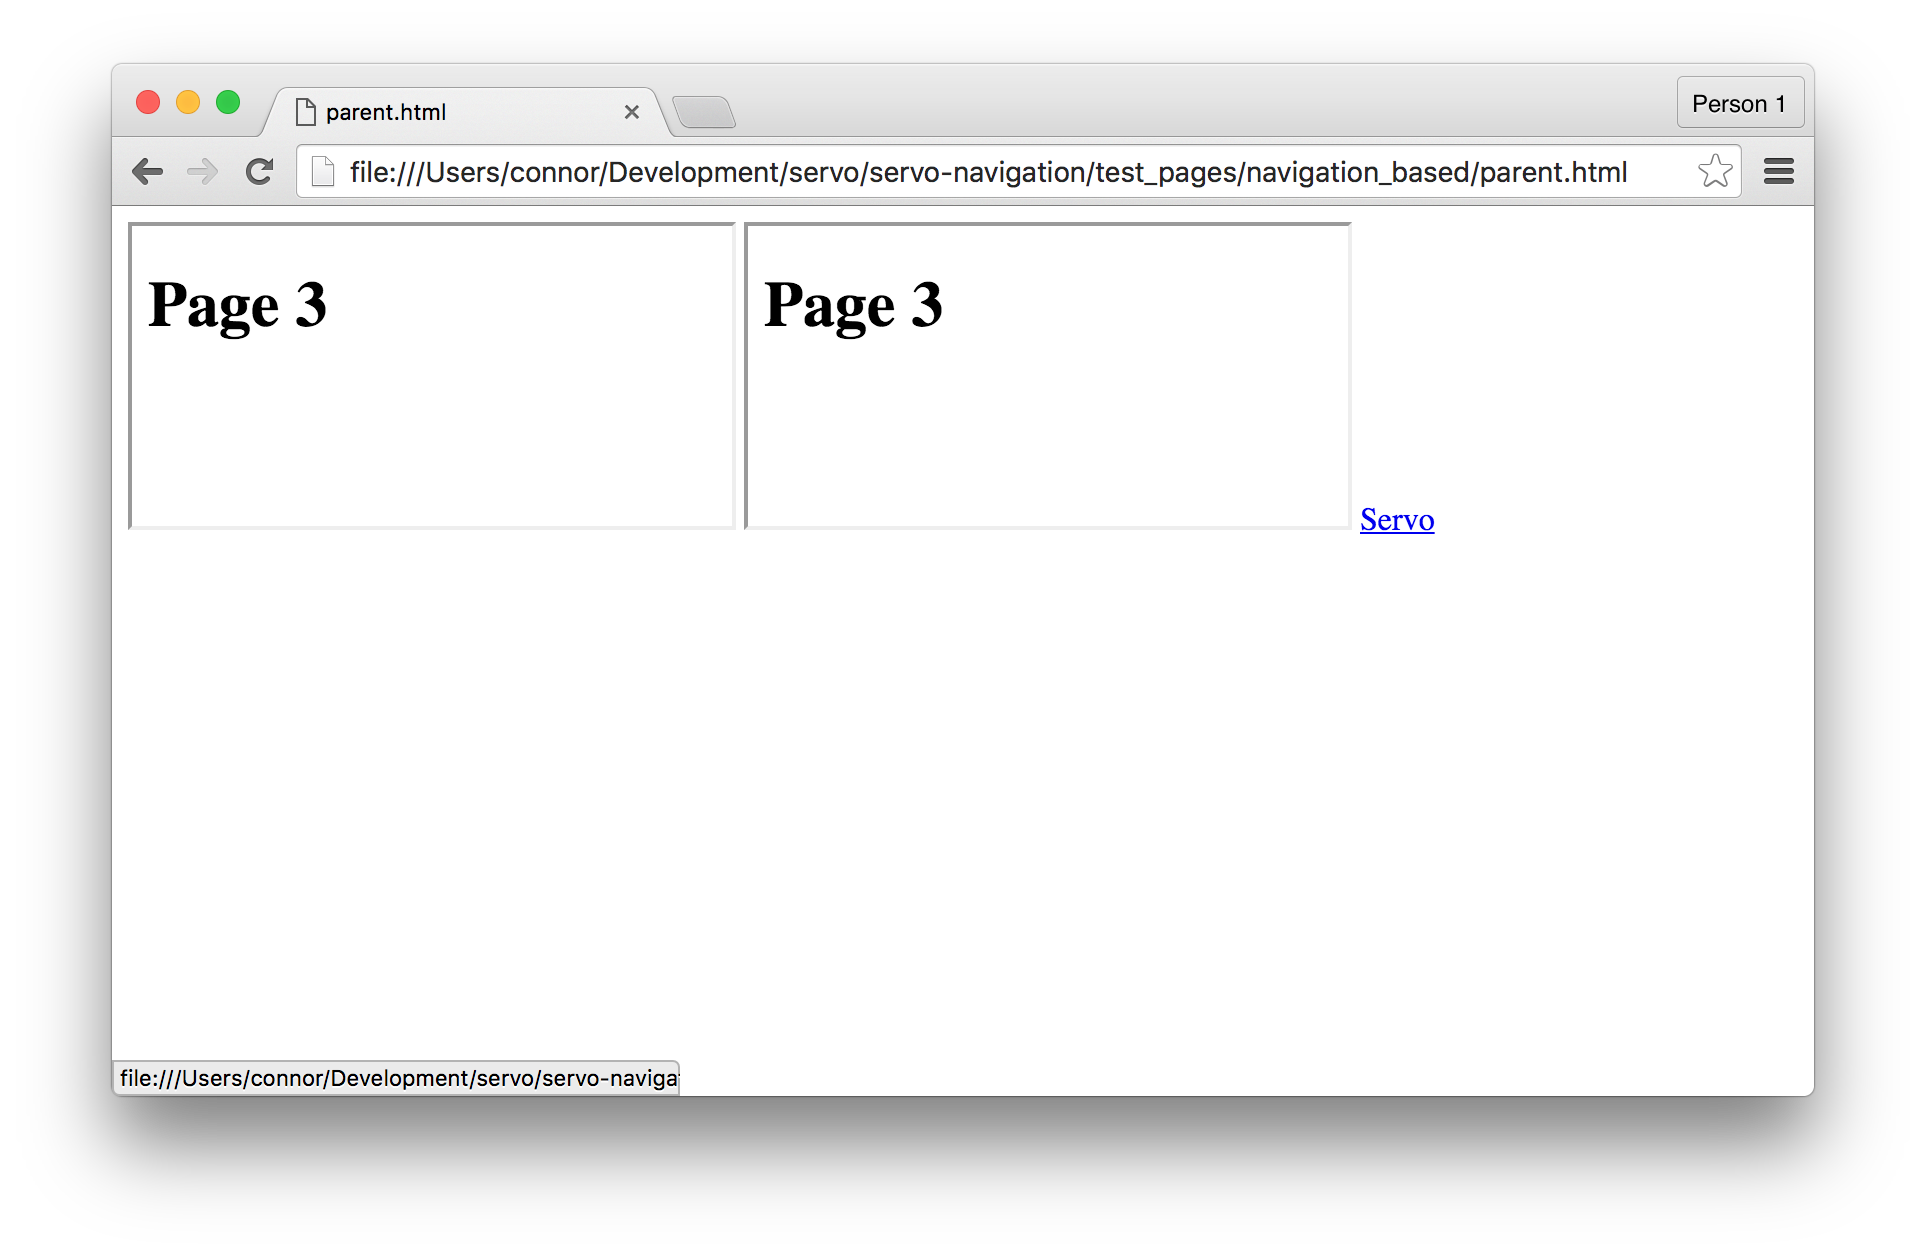
\includegraphics[width=.5\linewidth]{images/experiments/forwardback4/chrome/5.png}
    }~\raisebox{-.5\height}{
      \begin{tikzpicture}
        \node[doc,active,fully](0) at (0,0){0};
        \node[doc](1) at (1,-1){1};
        \node[doc](2) at (2,-2){2};
        \node[doc](3) at (3,-1){3};
        \node[doc,active,fully](4) at (4,-1){4};
        \node[doc](5) at (5,-2){5};
        \node[doc,jshactive,fully](6) at (6,-2){6};
        \node[draw,dotted,fit=(0)]{};
        \node[draw,dotted,fit=(1)(4)]{};
        \node[draw,dotted,fit=(2)(6)]{};
        \draw[->](0)to[out=0,in=140](4);
        \draw[->](0)to[out=0,in=120](6);
      \end{tikzpicture}
    }
    \caption{Navigate document $5$ to Page 3.}
  \end{figure}

  \emph{$\aNH$ traverses the history by $-4$ to $\aNH'$}:
  \begin{figure}[H]
    \raisebox{-.5\height}{
      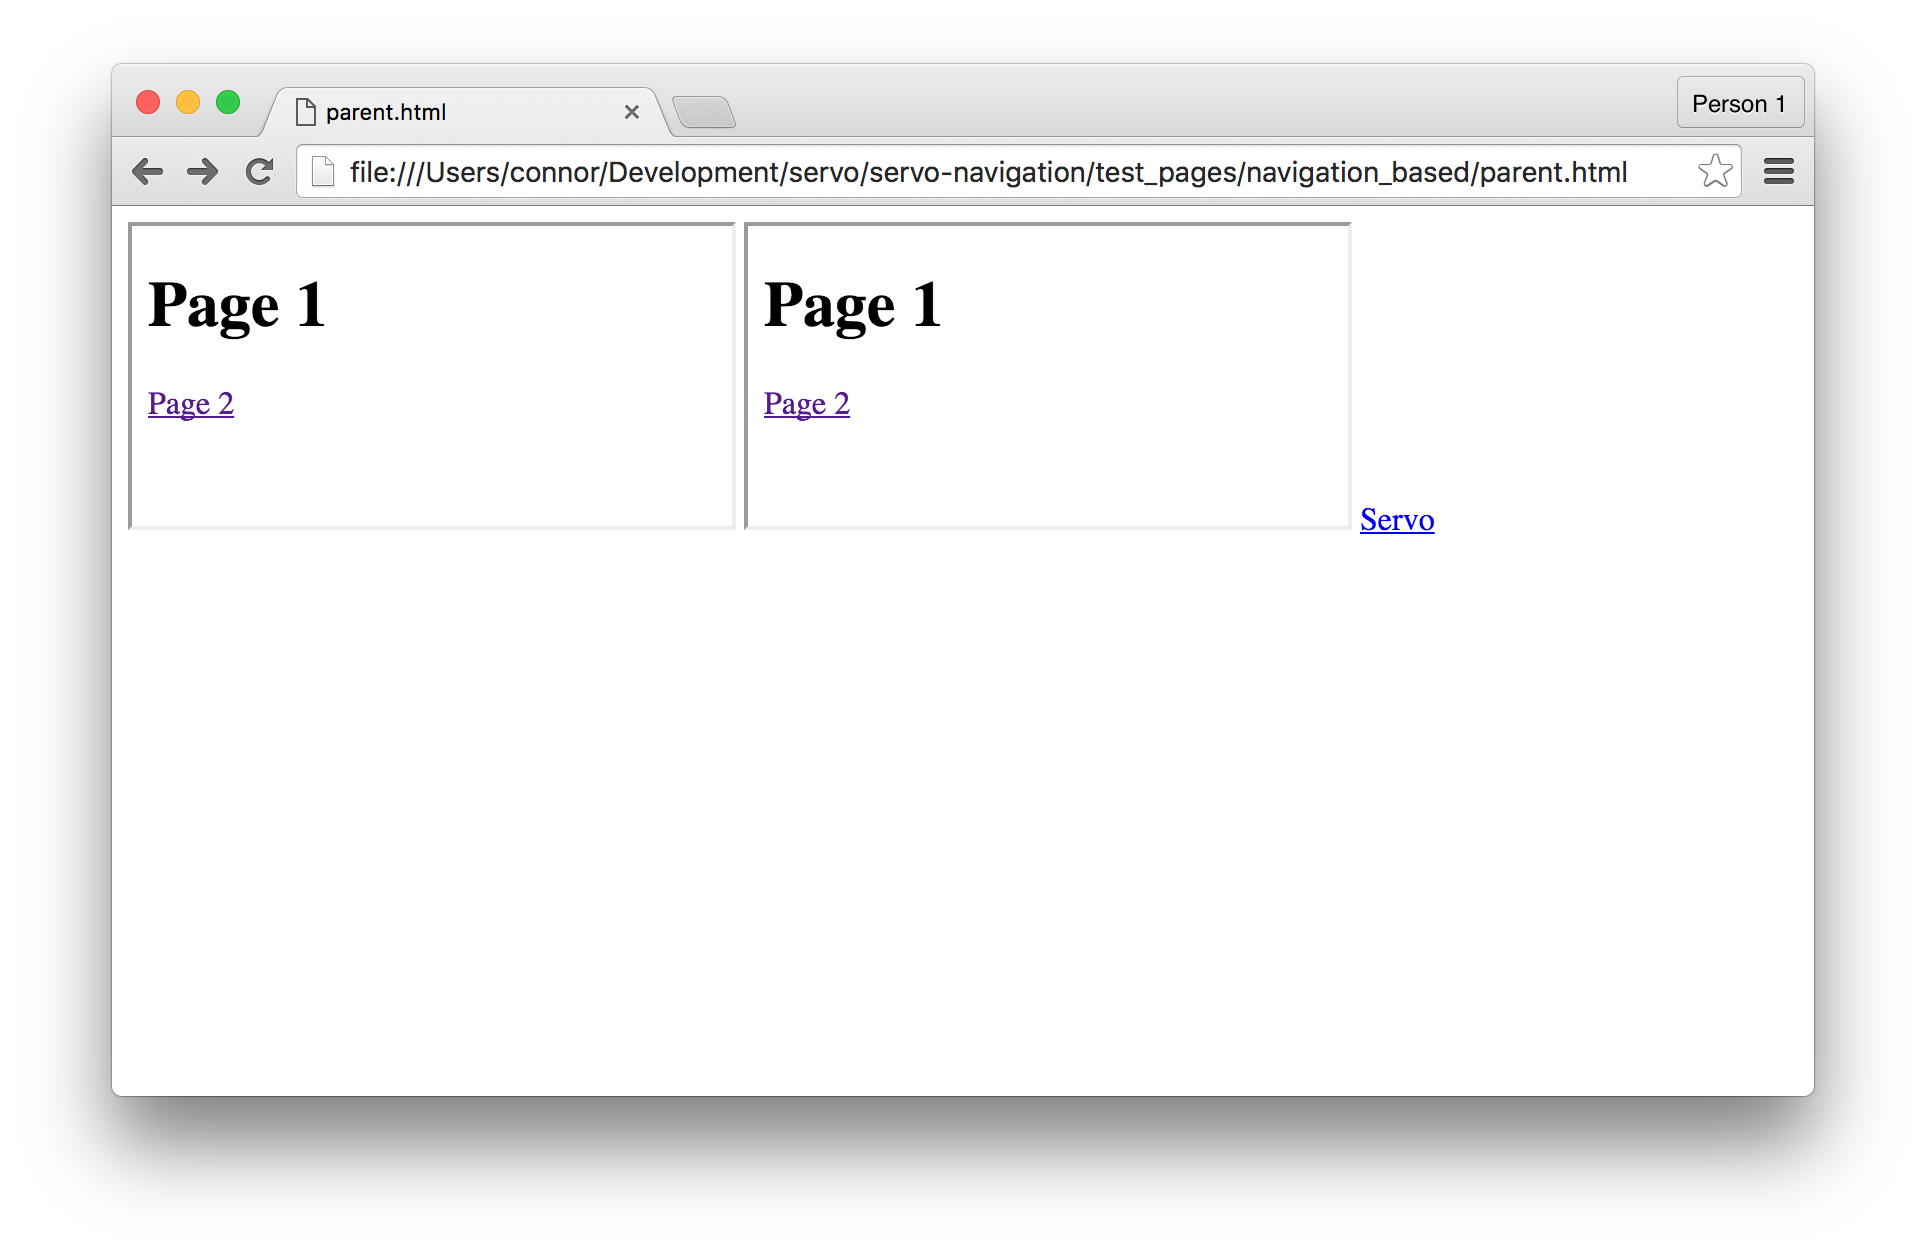
\includegraphics[width=.5\linewidth]{images/experiments/forwardback4/chrome/6.png}
    }~\raisebox{-.5\height}{
      \begin{tikzpicture}
        \node[doc,active,fully](0) at (0,0){0};
        \node[doc,active,fully](1) at (1,-1){1};
        \node[doc,jshactive,fully](2) at (2,-2){2};
        \node[doc](3) at (3,-1){3};
        \node[doc](4) at (4,-1){4};
        \node[doc](5) at (5,-2){5};
        \node[doc](6) at (6,-2){6};
        \node[draw,dotted,fit=(0)]{};
        \node[draw,dotted,fit=(1)(4)]{};
        \node[draw,dotted,fit=(2)(6)]{};
        \draw[->](0)--(1);
        \draw[->](0)to[out=-20,in=90](2);
      \end{tikzpicture}
    }
    \caption{Traversal by $-4$.}
  \end{figure}

  \emph{$\aNH'$ traverses the history by $4$ to $\aNH''$}:
  \begin{figure}[H]
    \raisebox{-.5\height}{
      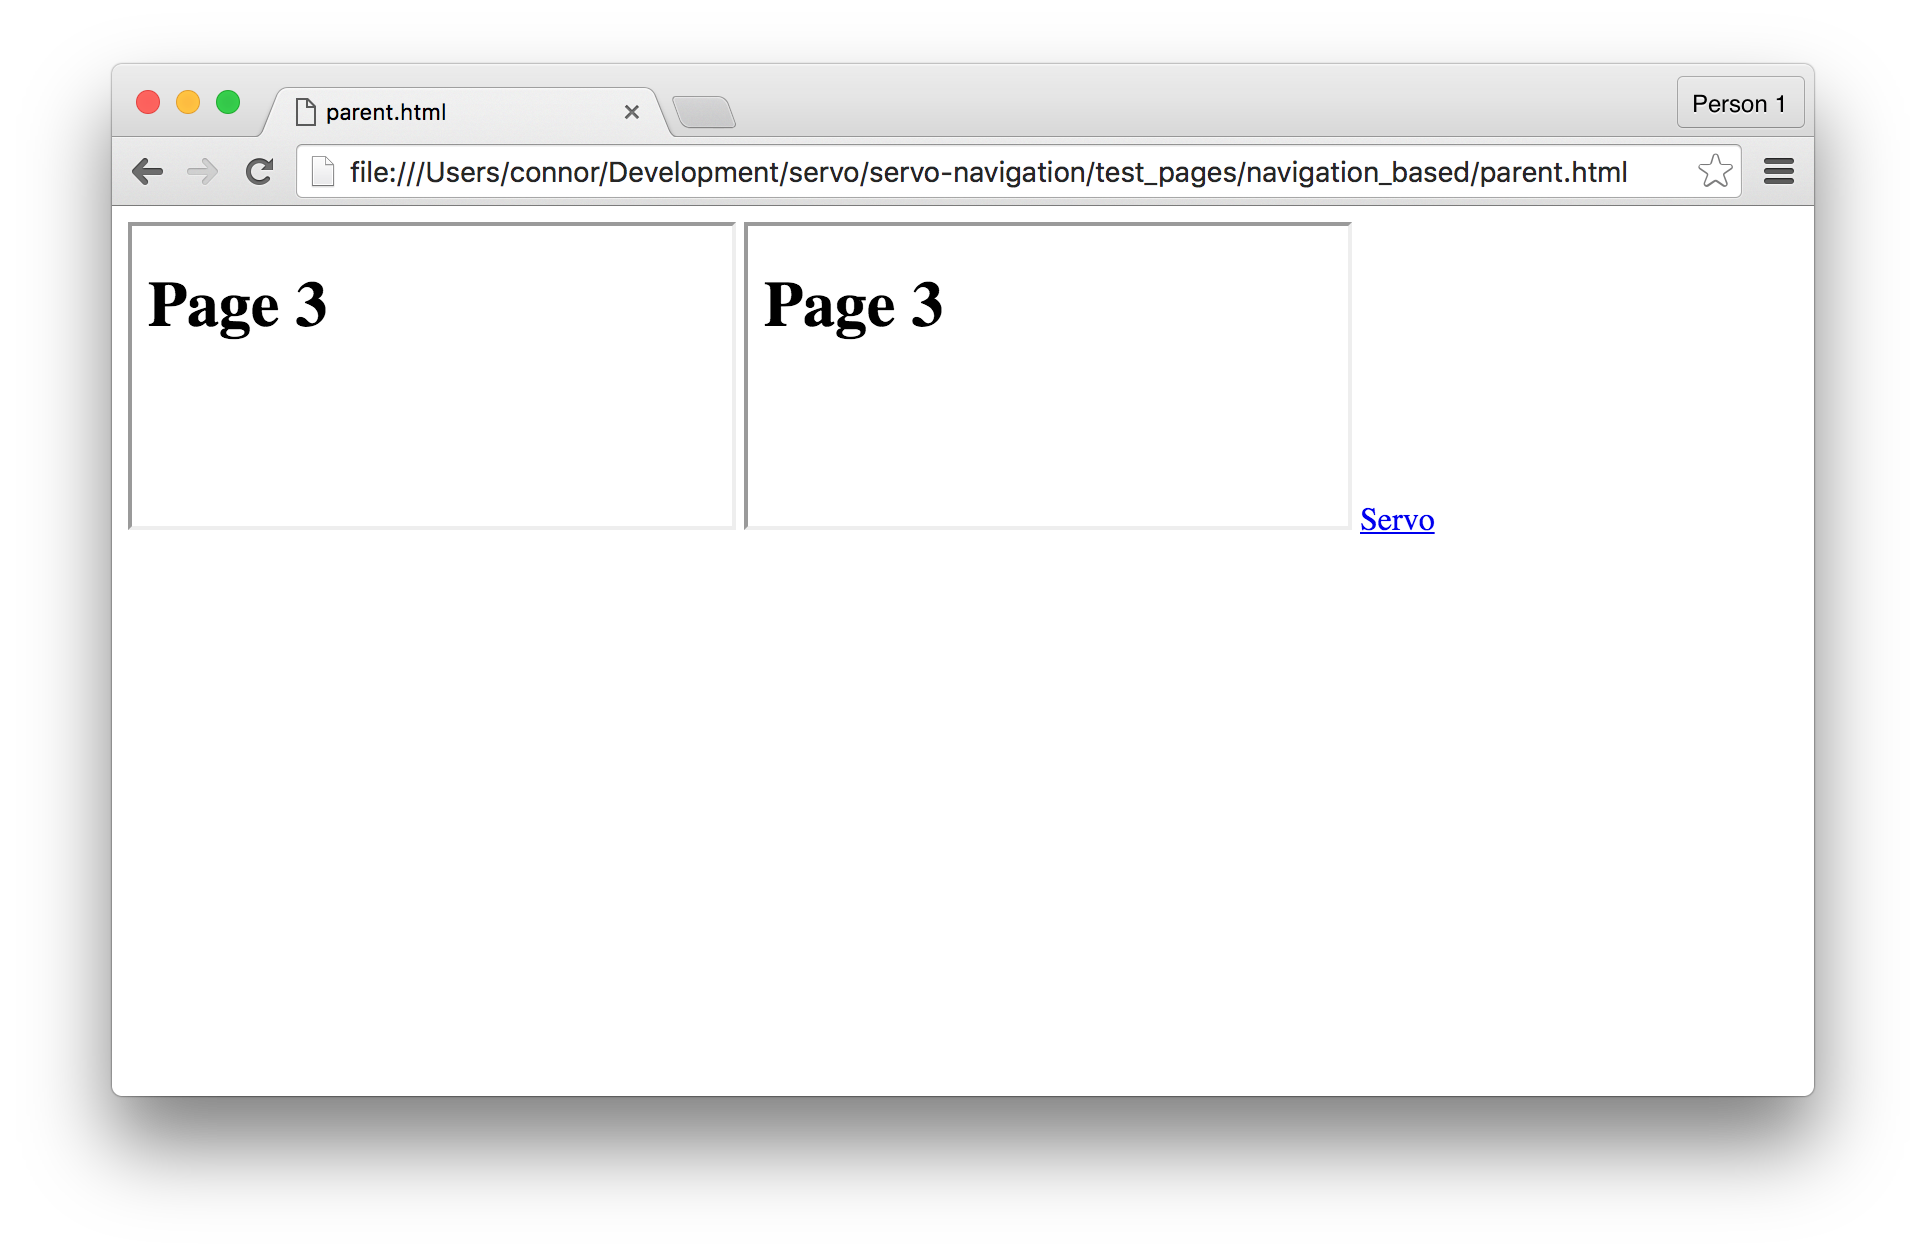
\includegraphics[width=.5\linewidth]{images/experiments/forwardback4/chrome/7.png}
    }~\raisebox{-.5\height}{
      \begin{tikzpicture}
        \node[doc,active,fully](0) at (0,0){0};
        \node[doc](1) at (1,-1){1};
        \node[doc](2) at (2,-2){2};
        \node[doc](3) at (3,-1){3};
        \node[doc,active,fully](4) at (4,-1){4};
        \node[doc](5) at (5,-2){5};
        \node[doc,jshactive,fully](6) at (6,-2){6};
        \node[draw,dotted,fit=(0)]{};
        \node[draw,dotted,fit=(1)(4)]{};
        \node[draw,dotted,fit=(2)(6)]{};
        \draw[->](0)to[out=0,in=140](4);
        \draw[->](0)to[out=0,in=120](6);
      \end{tikzpicture}
    }
    \caption{Traversal by $4$.}
  \end{figure}

  These results in Chrome satisfy Goal~\ref{goal:homomorphism}.
\end{experiment}

\begin{experiment}
  In this experiment $pushState$ and $replaceState$ traversals are tested against Goal~\ref{goal:homomorphism}.

  Firefox:
  \begin{figure}[H]
    \raisebox{-.5\height}{
      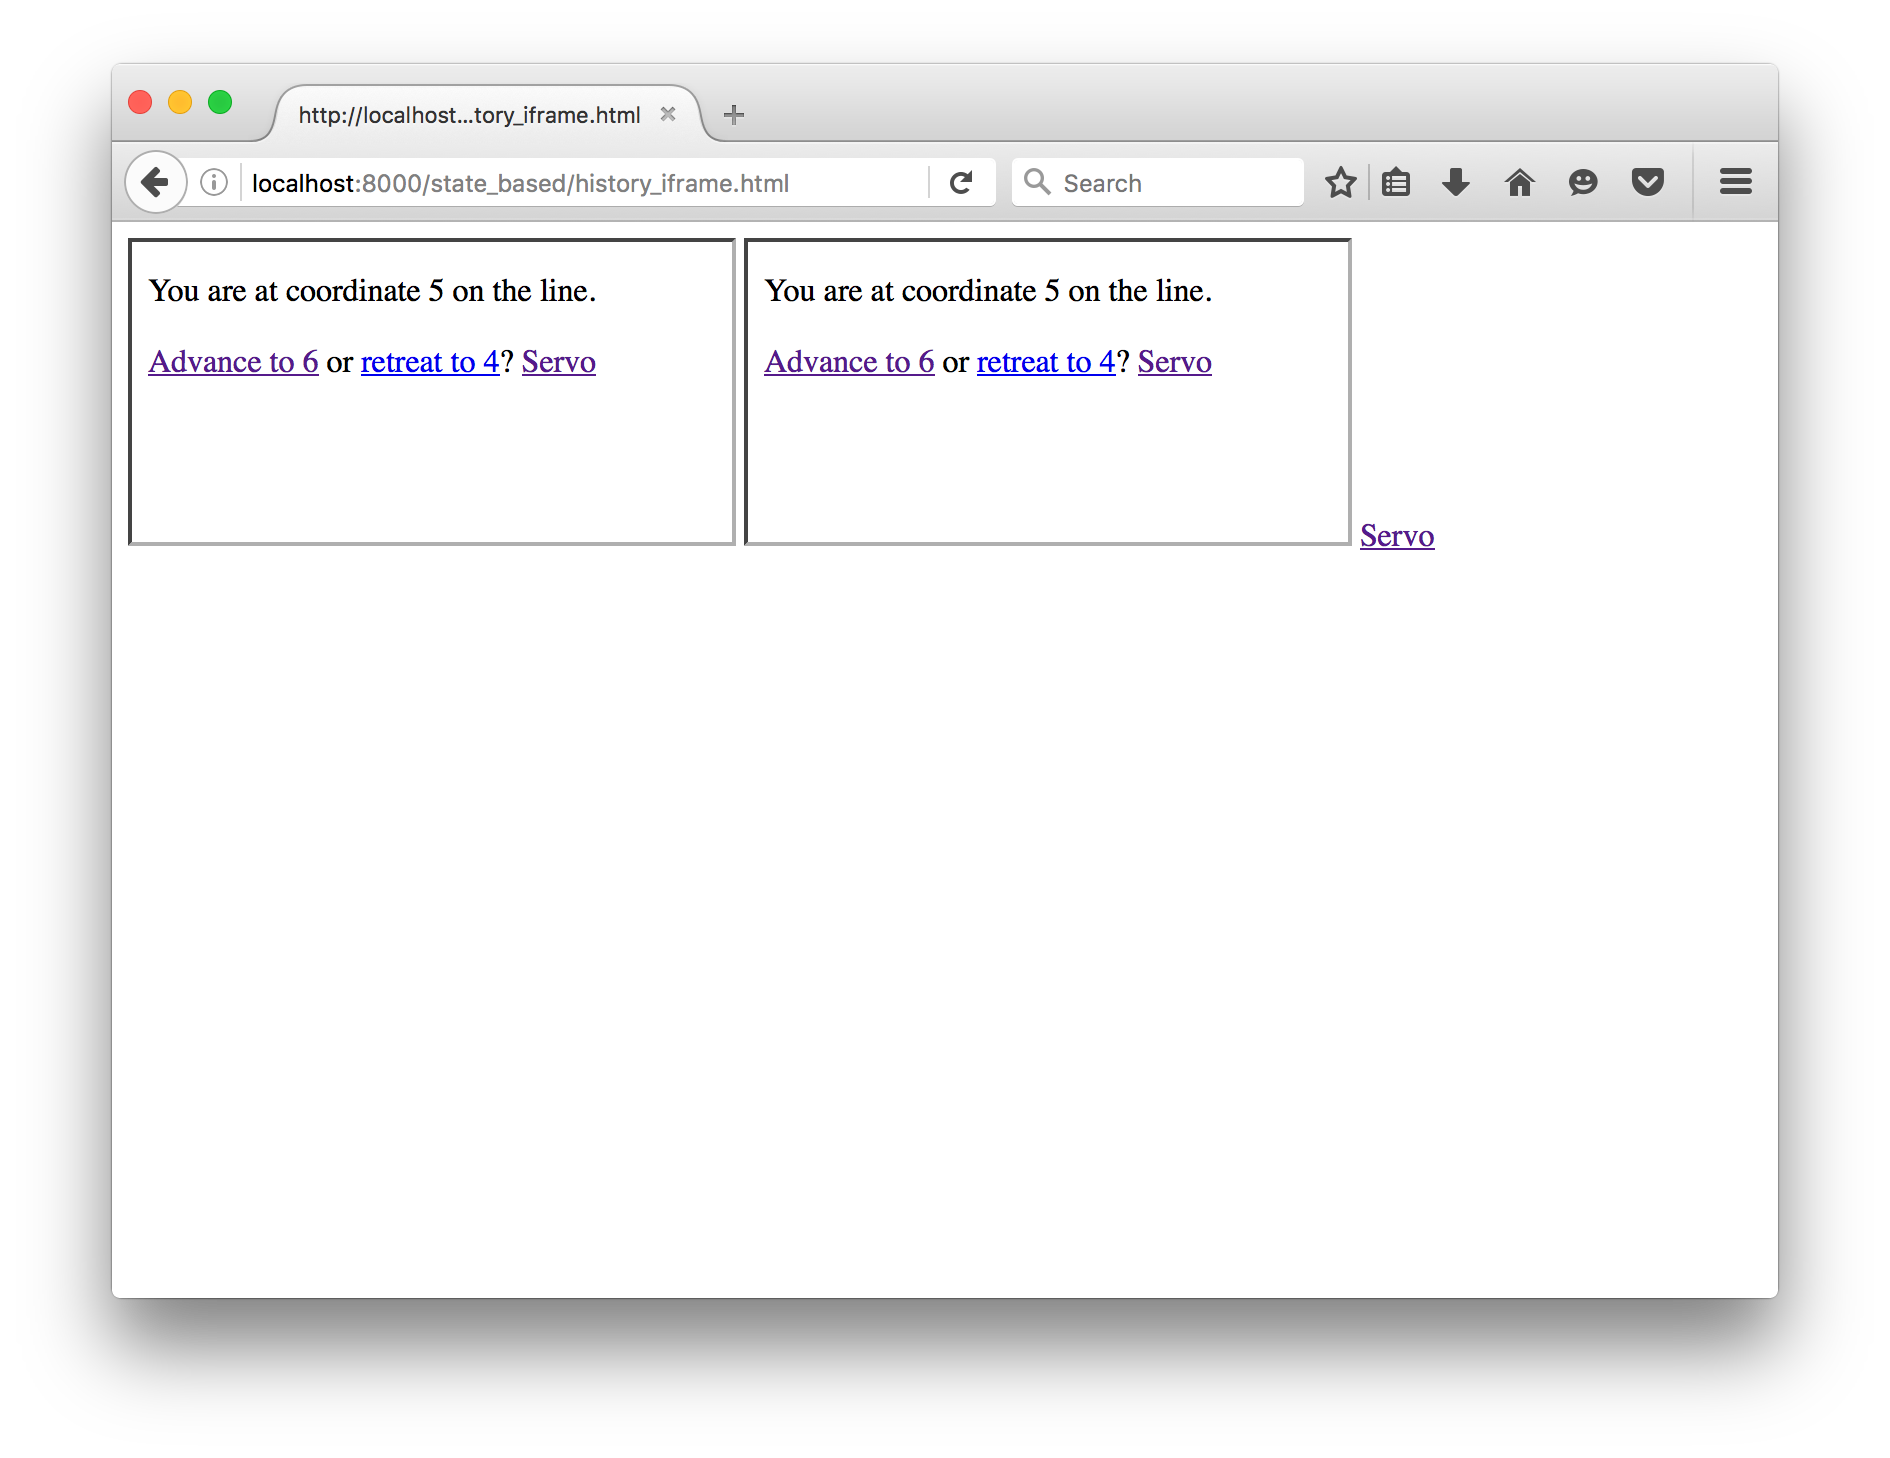
\includegraphics[width=.5\linewidth]{images/experiments/forwardback4state/firefox/1.png}%
    }~\raisebox{-.5\height}{
      \begin{tikzpicture}
        \node[doc,active,fully](0) at (0,0){0};
        \node[doc,active,fully](1) at (1,-1){1};
        \node[doc,jshactive,fully](2) at (2,-2){2};
        \node[draw,dotted,fit=(0)]{};
        \node[draw,dotted,fit=(1)]{};
        \node[draw,dotted,fit=(2)]{};
        \draw[->](0)--(1);
        \draw[->](0)to[out=-20,in=90](2);
      \end{tikzpicture}
    }
    \caption{Initial State}
  \end{figure}

  Advance document 1 to $6$:
  \begin{figure}[H]
    \raisebox{-.5\height}{
      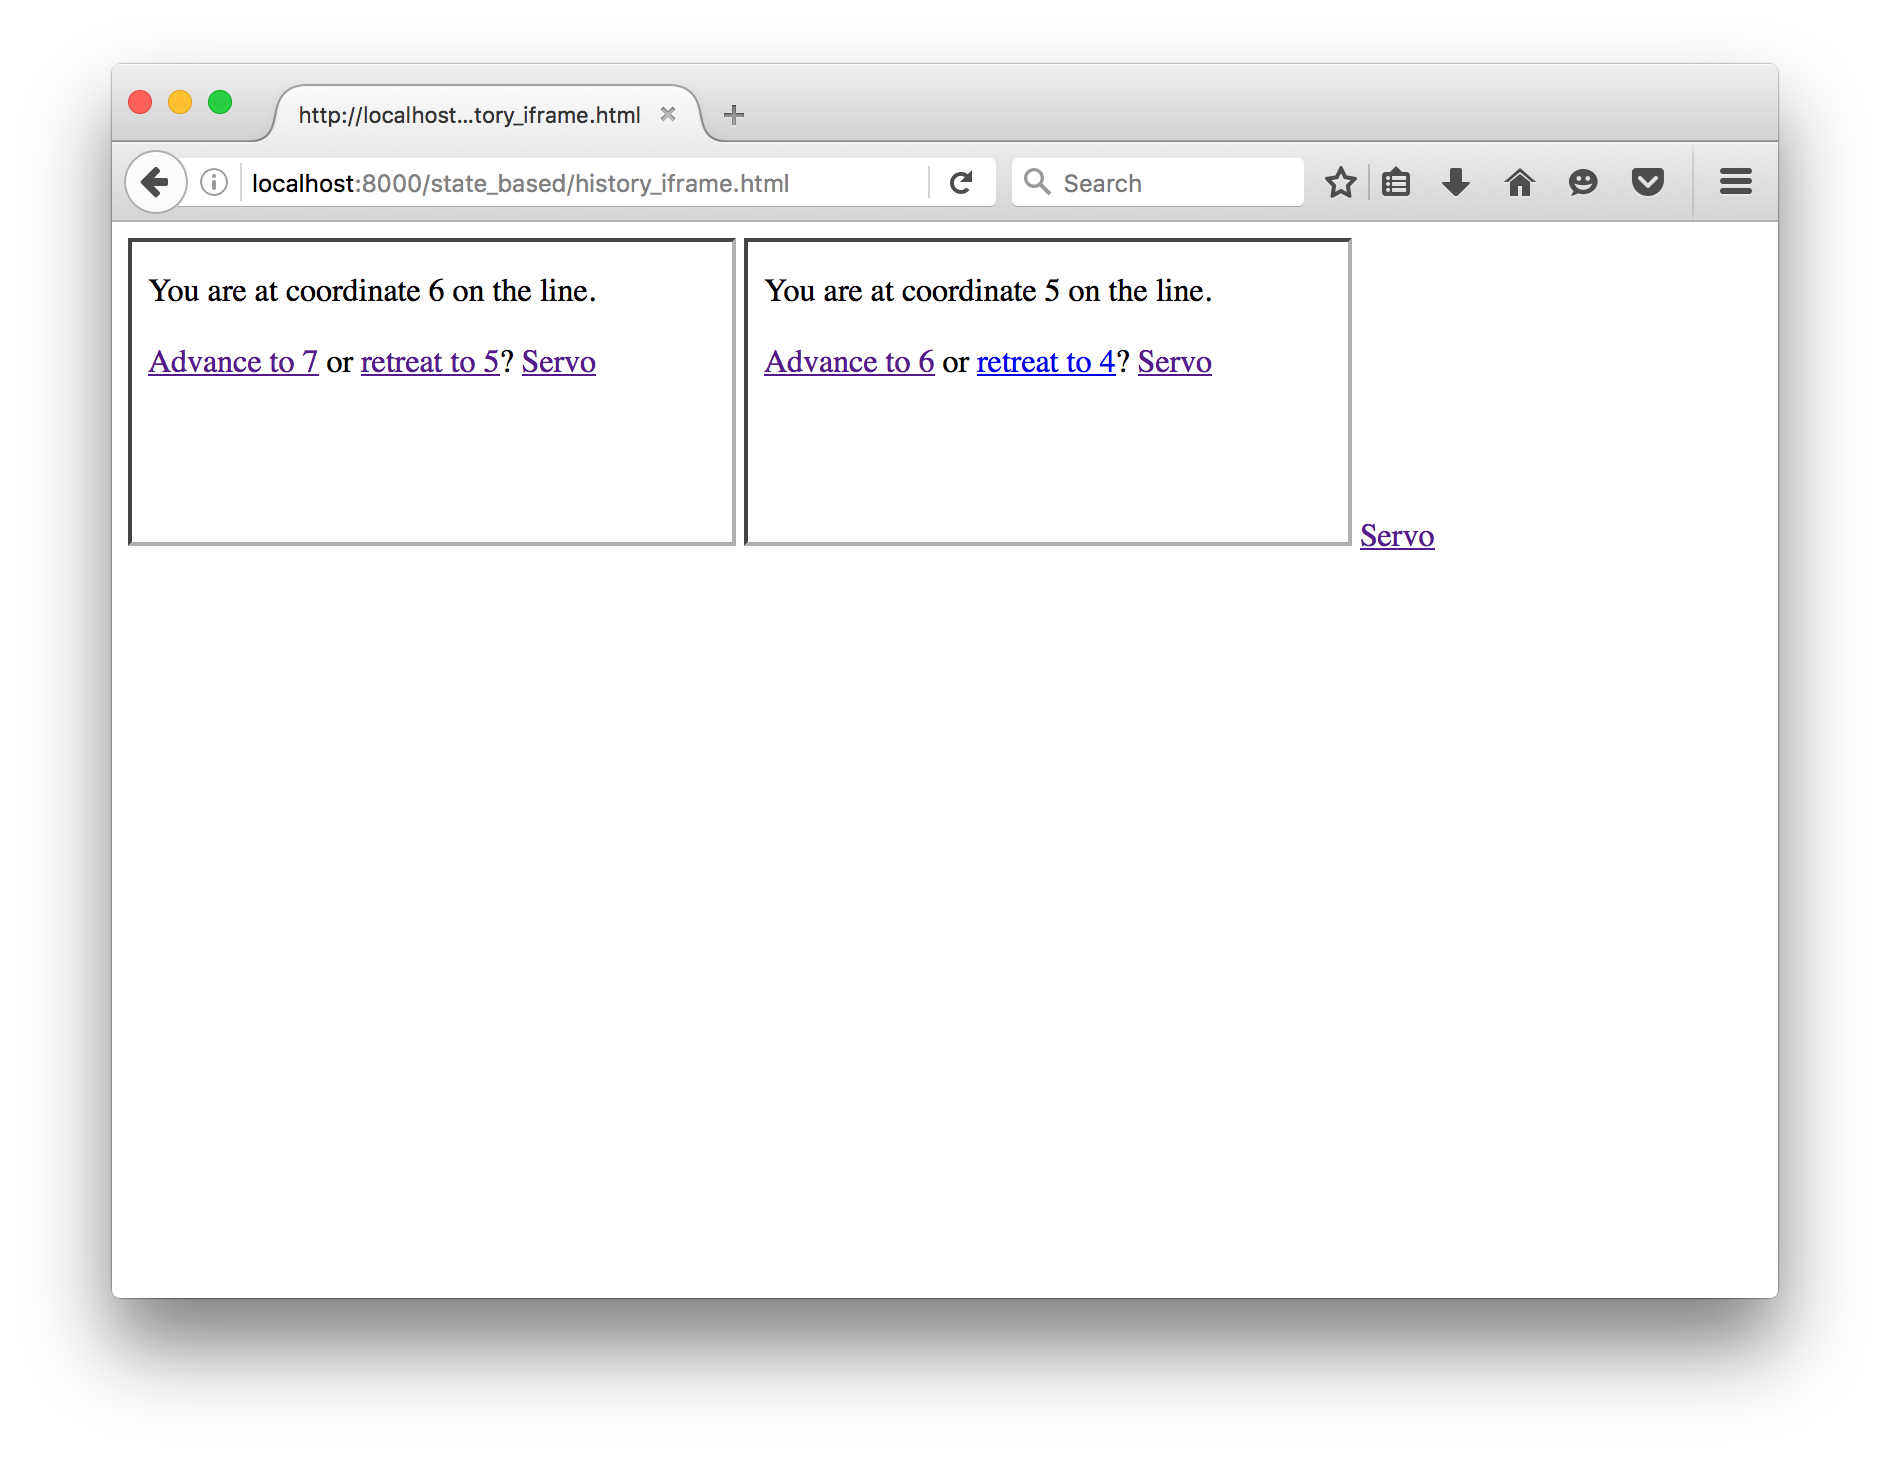
\includegraphics[width=.5\linewidth]{images/experiments/forwardback4state/firefox/2.png}%
    }~\raisebox{-.5\height}{
      \begin{tikzpicture}
        \node[doc,active,fully](0) at (0,0){0};
        \node[doc](1) at (1,-1){1};
        \node[doc,active,fully](2) at (2,-2){2};
        \node[doc,jshactive,fully](3) at (3,-1){3};
        \node[draw,dotted,fit=(0)]{};
        \node[draw,dotted,fit=(1)(3)]{};
        \node[draw,dotted,fit=(2)]{};
        \draw[->](0)--(3);
        \draw[->](0)to[out=-20,in=90](2);
      \end{tikzpicture}
    }
    \caption{Advance document 1 to $6$}
  \end{figure}

  Advance document 3 to $7$:
  \begin{figure}[H]
    \raisebox{-.5\height}{
      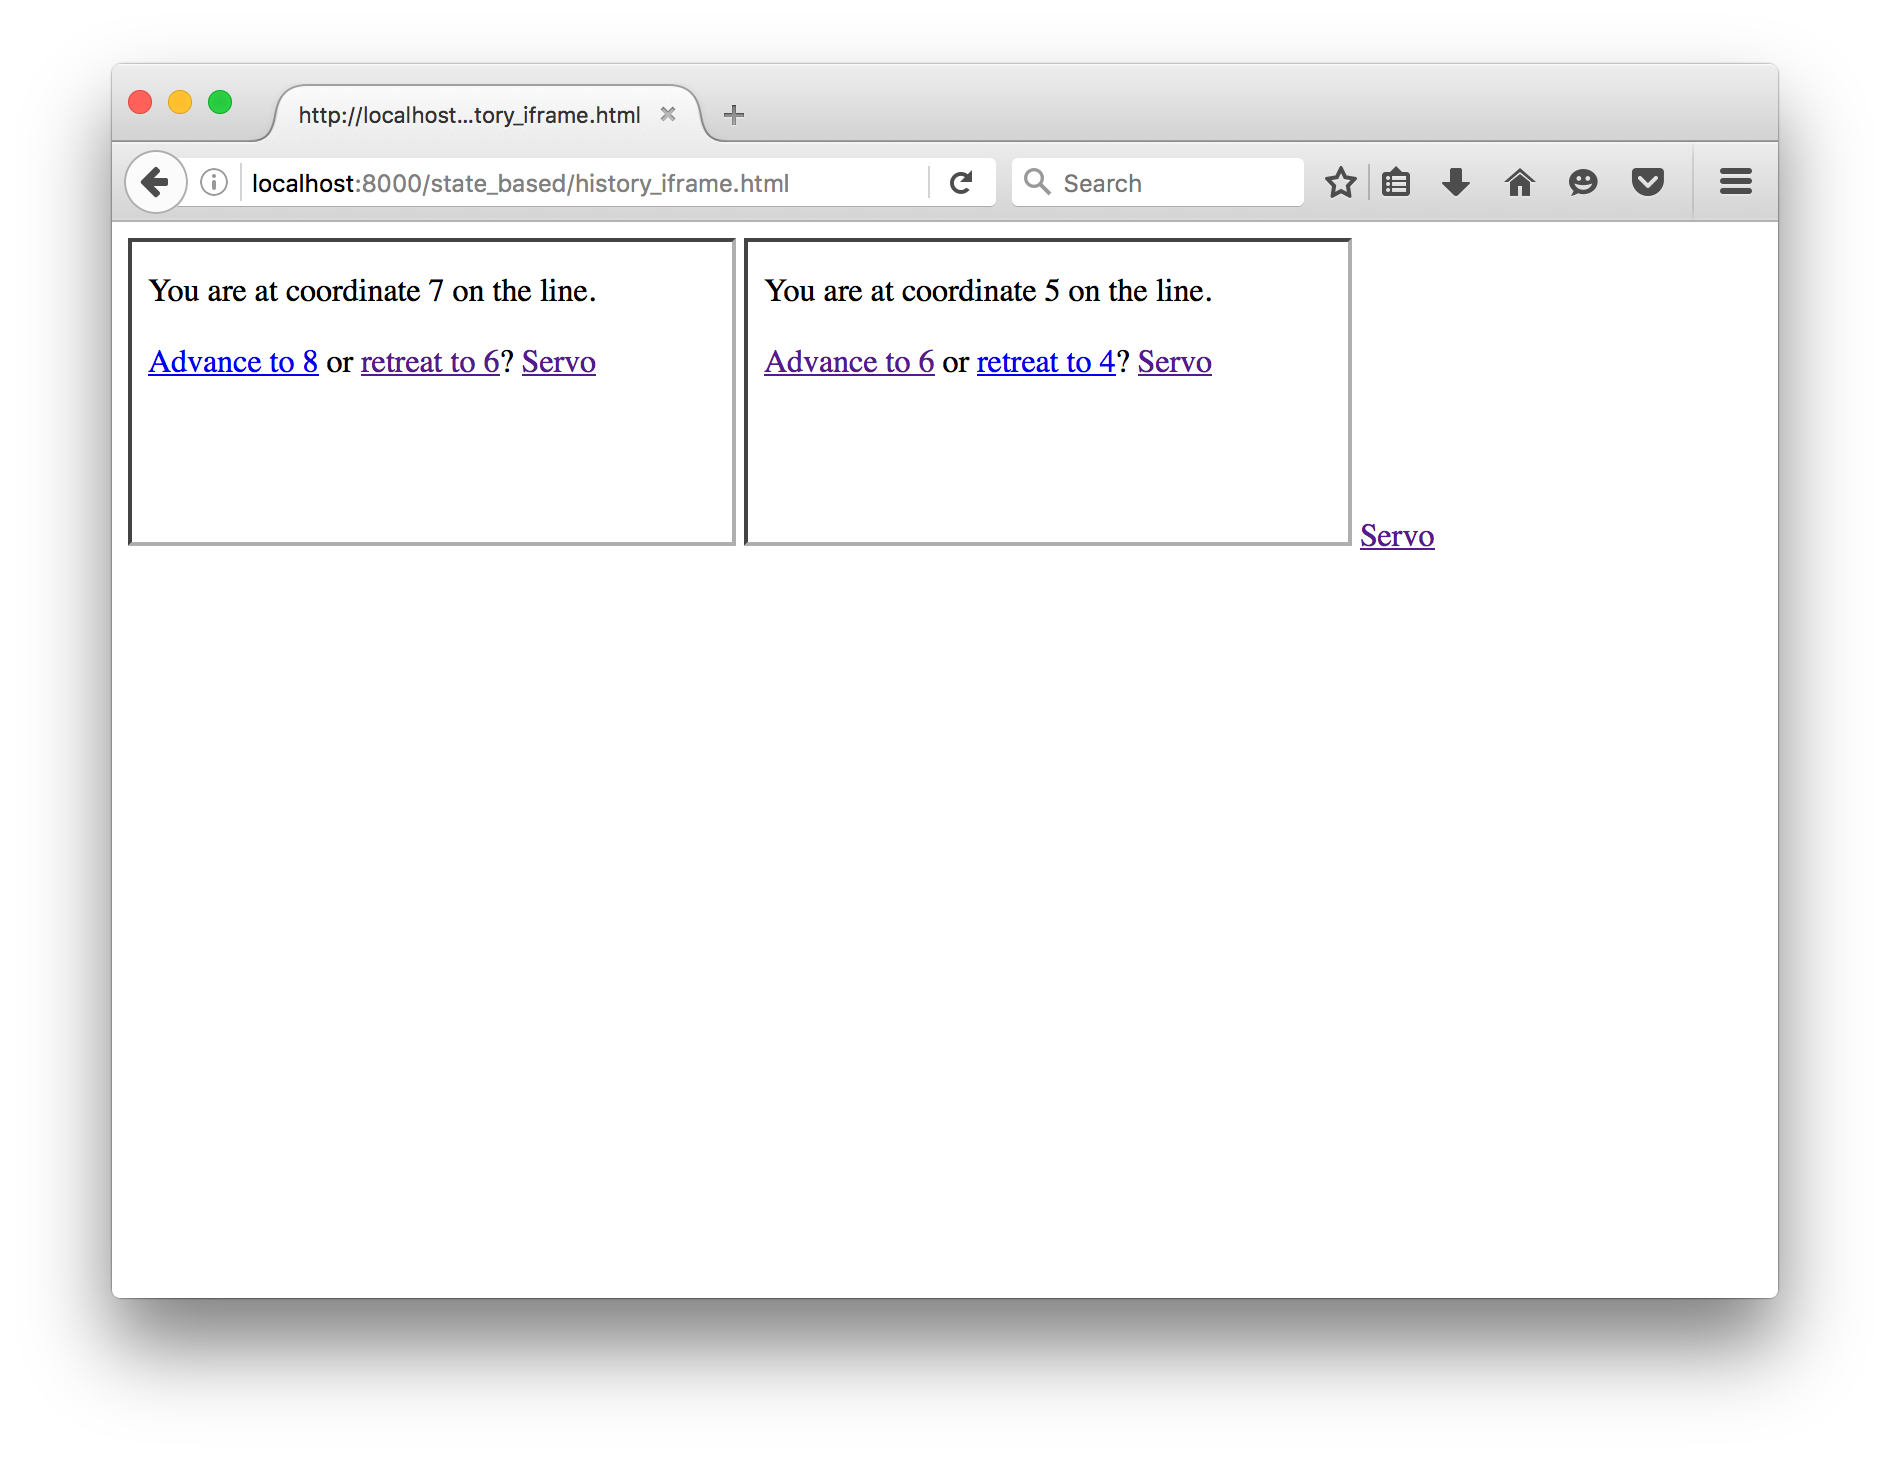
\includegraphics[width=.5\linewidth]{images/experiments/forwardback4state/firefox/3.png}%
    }~\raisebox{-.5\height}{
      \begin{tikzpicture}
        \node[doc,active,fully](0) at (0,0){0};
        \node[doc](1) at (1,-1){1};
        \node[doc,active,fully](2) at (2,-2){2};
        \node[doc](3) at (3,-1){3};
        \node[doc,jshactive,fully](4) at (4,-1){4};
        \node[draw,dotted,fit=(0)]{};
        \node[draw,dotted,fit=(1)(4)]{};
        \node[draw,dotted,fit=(2)]{};
        \draw[->](0)to[out=0,in=140](4);
        \draw[->](0)to[out=-20,in=90](2);
      \end{tikzpicture}
    }
    \caption{Advance document 3 to $7$}
  \end{figure}

  Advance document 2 to $6$:
  \begin{figure}[H]
    \raisebox{-.5\height}{
      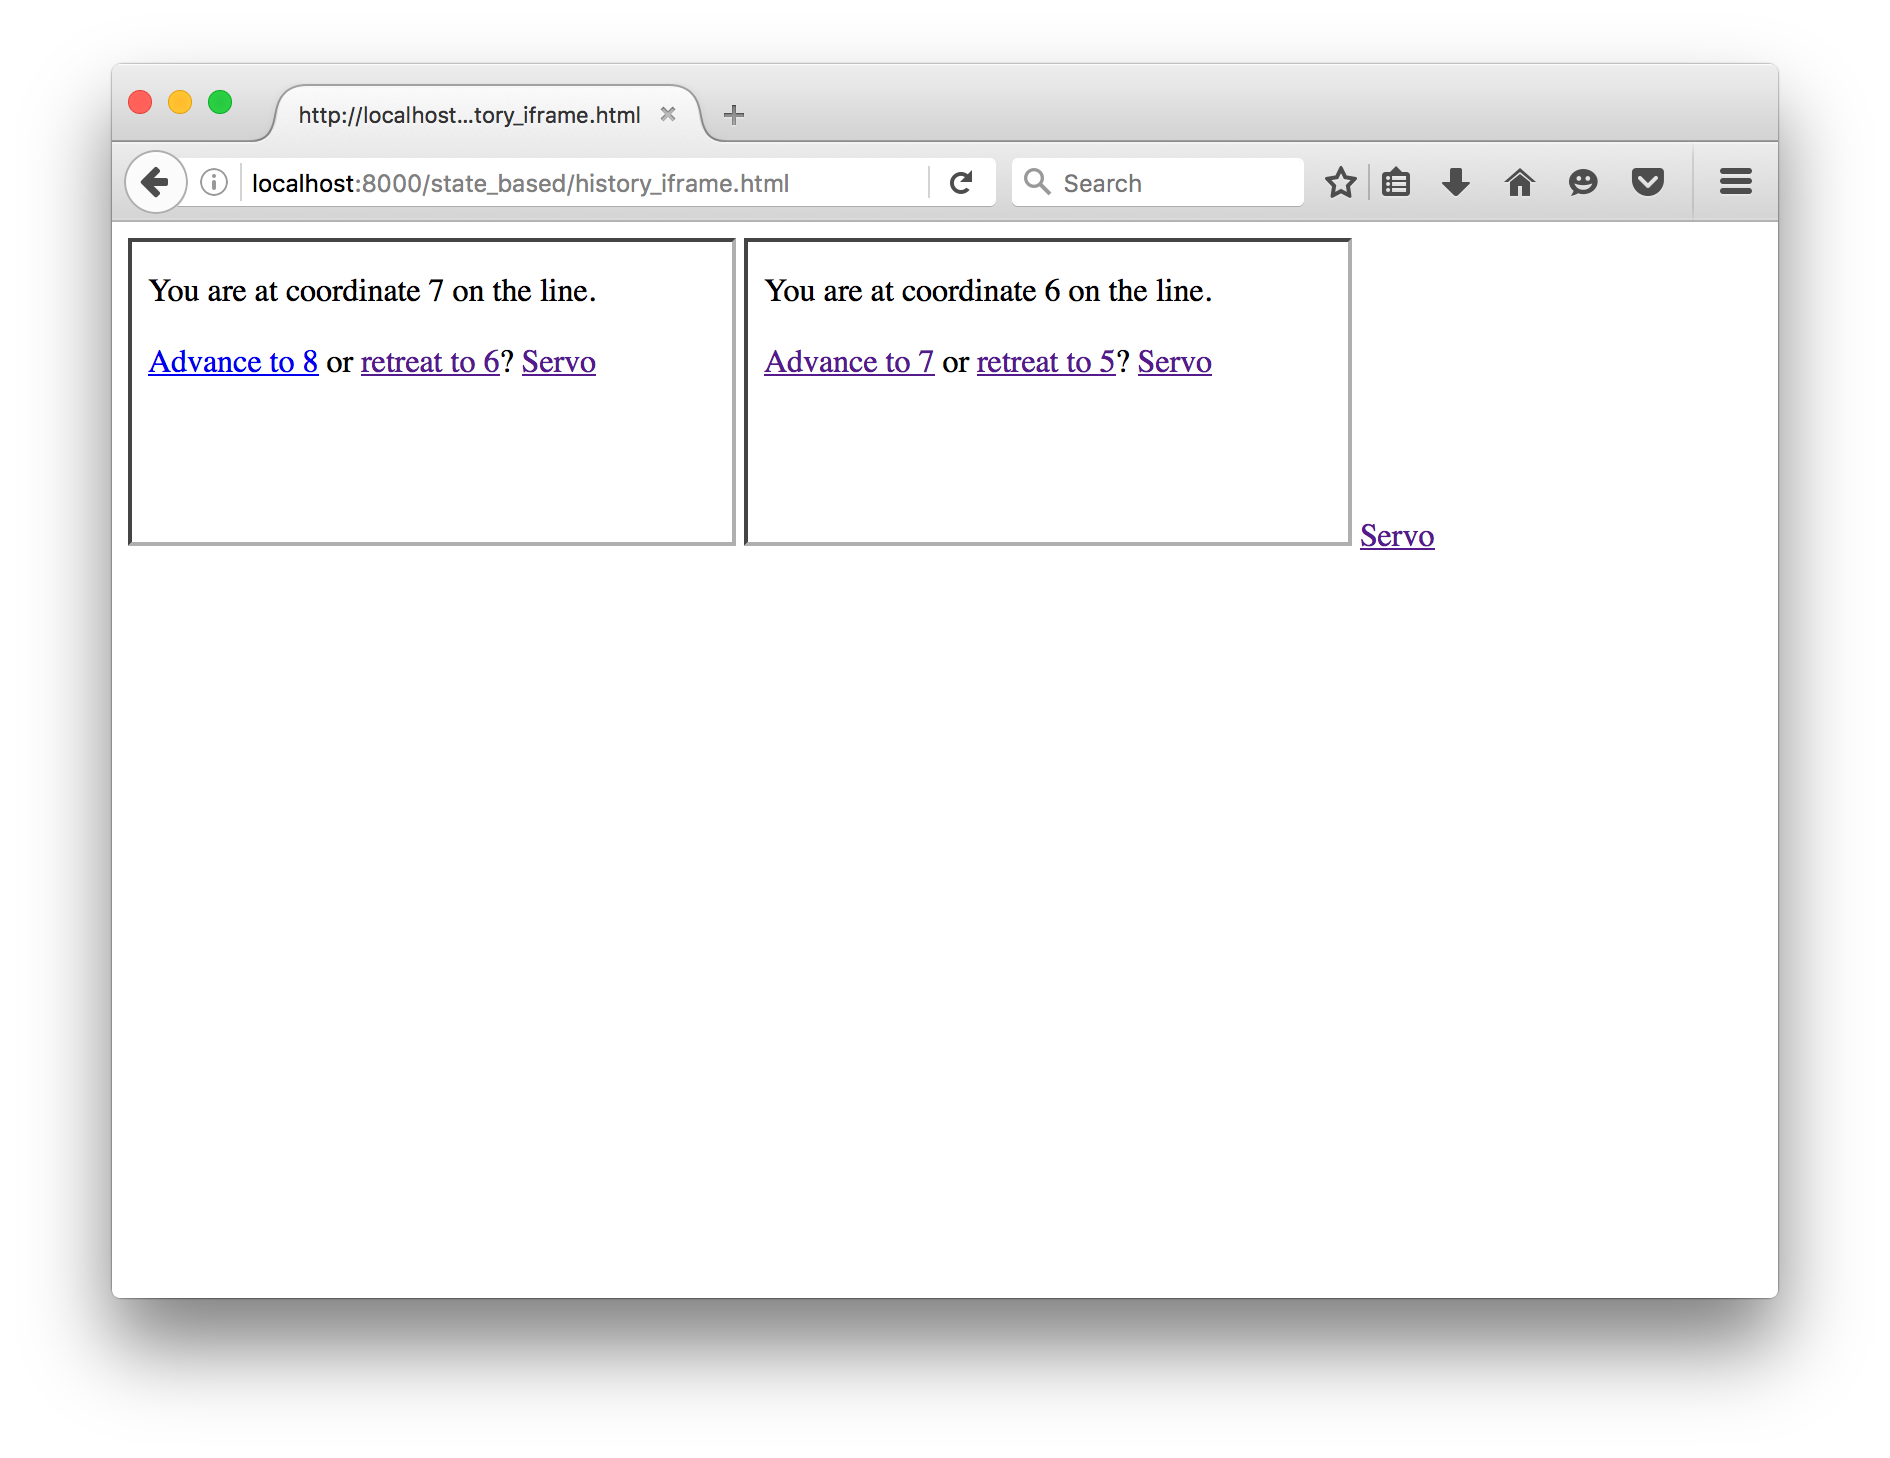
\includegraphics[width=.5\linewidth]{images/experiments/forwardback4state/firefox/4.png}%
    }~\raisebox{-.5\height}{
      \begin{tikzpicture}
        \node[doc,active,fully](0) at (0,0){0};
        \node[doc](1) at (1,-1){1};
        \node[doc](2) at (2,-2){2};
        \node[doc](3) at (3,-1){3};
        \node[doc,active,fully](4) at (4,-1){4};
        \node[doc,jshactive,fully](5) at (5,-2){5};
        \node[draw,dotted,fit=(0)]{};
        \node[draw,dotted,fit=(1)(4)]{};
        \node[draw,dotted,fit=(2)(5)]{};
        \draw[->](0)to[out=0,in=140](4);
        \draw[->](0)to[out=0,in=90](5);
      \end{tikzpicture}
    }
    \caption{Advance document $2$ to $6$}
  \end{figure}

  Advance $document 2$ to $7$:
  \begin{figure}[H]
    \raisebox{-.5\height}{
      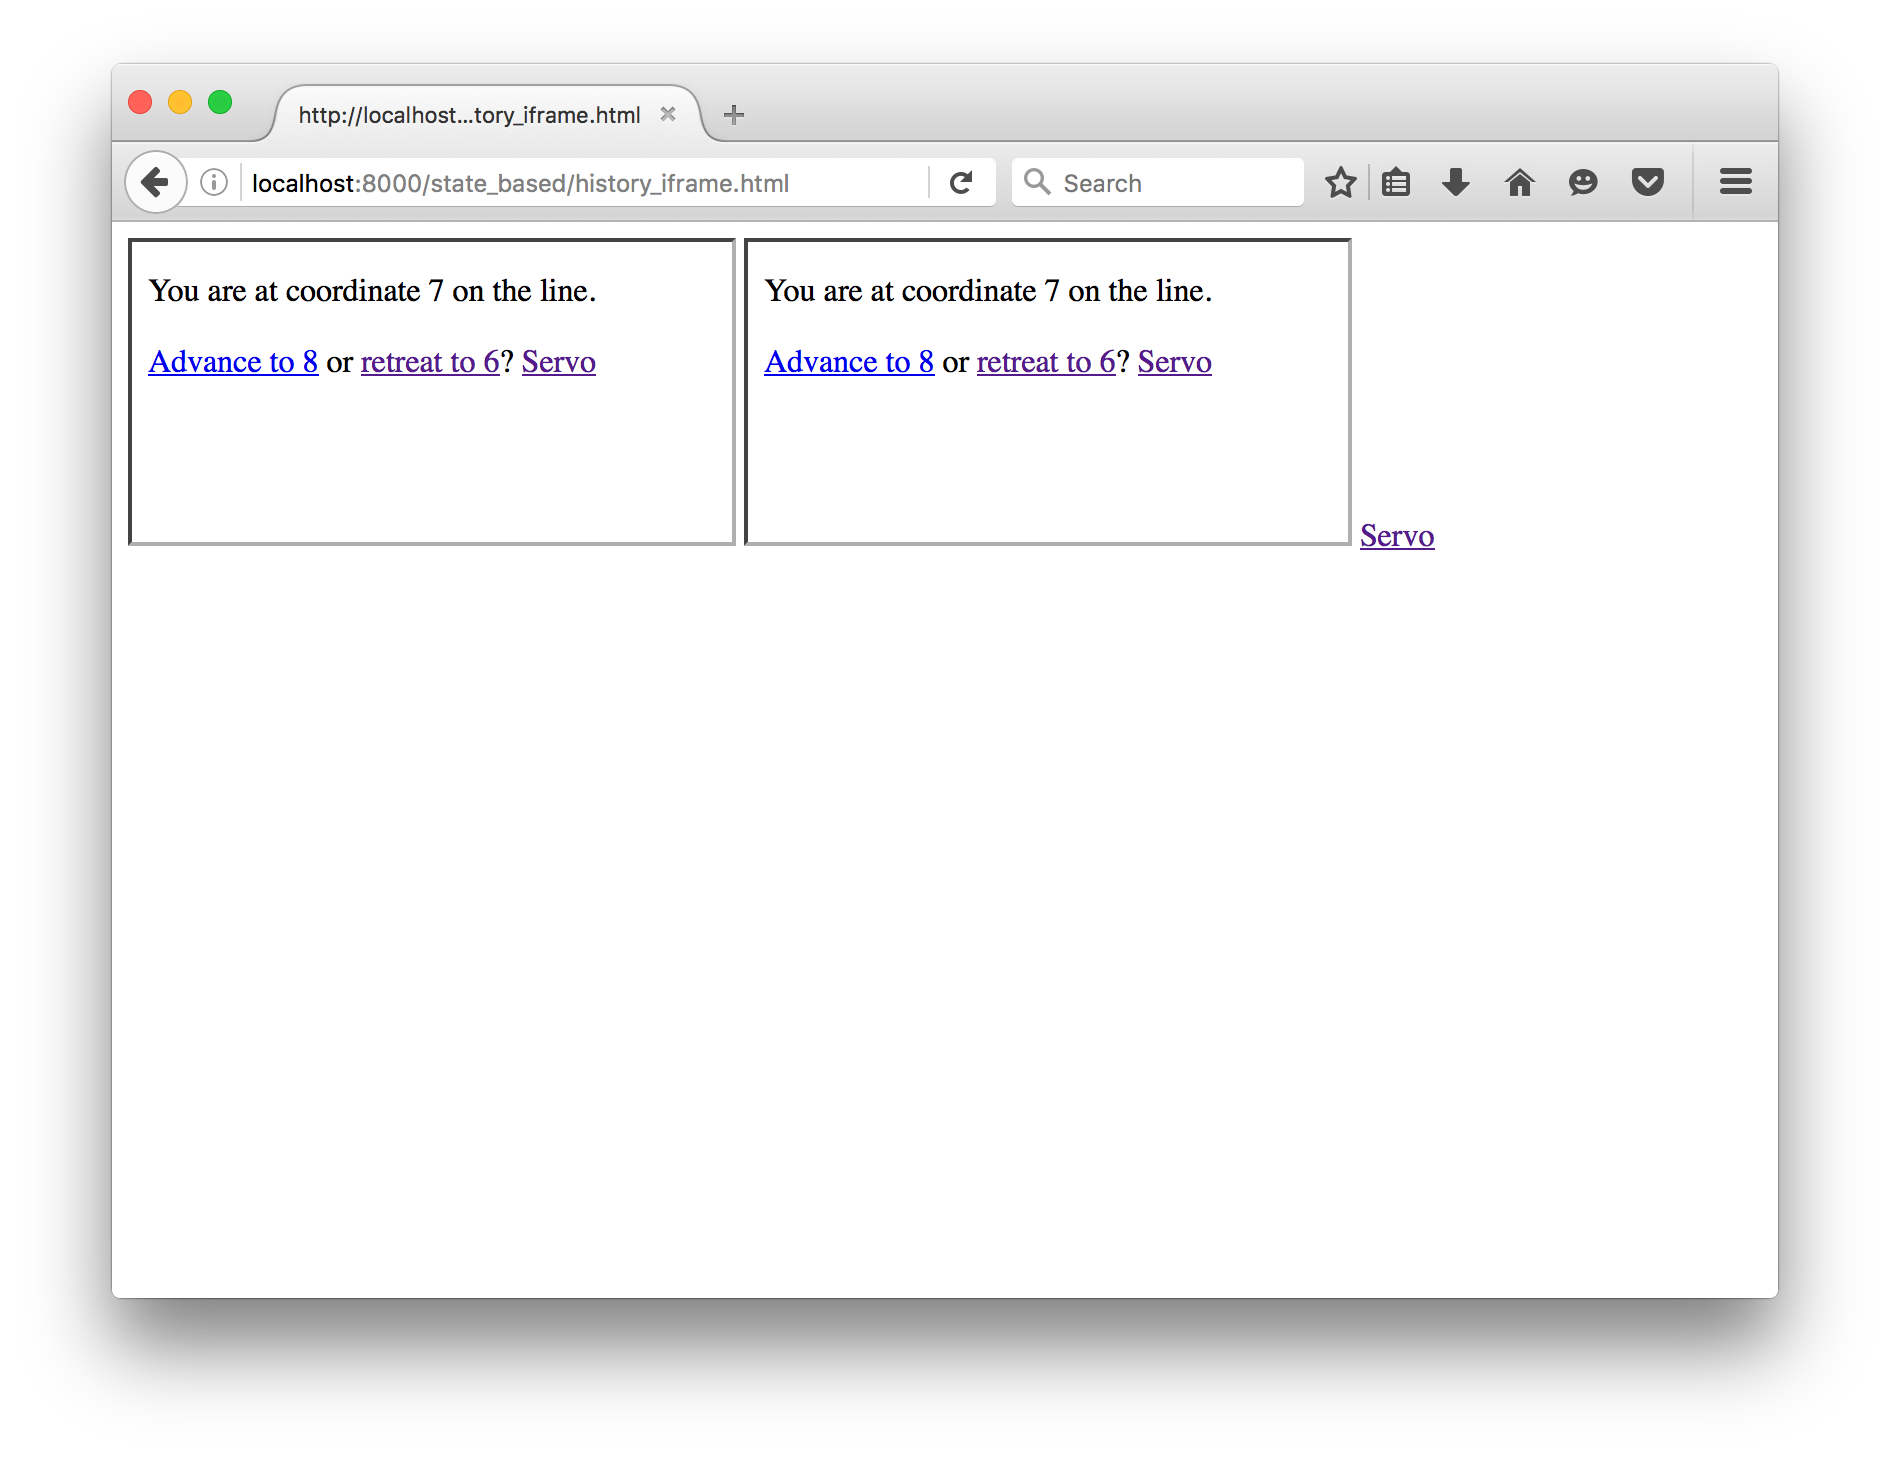
\includegraphics[width=.5\linewidth]{images/experiments/forwardback4state/firefox/5.png}%
    }~\raisebox{-.5\height}{
      \begin{tikzpicture}
        \node[doc,active,fully](0) at (0,0){0};
        \node[doc](1) at (1,-1){1};
        \node[doc](2) at (2,-2){2};
        \node[doc](3) at (3,-1){3};
        \node[doc,active,fully](4) at (4,-1){4};
        \node[doc](5) at (5,-2){5};
        \node[doc,jshactive,fully](6) at (6,-2){6};
        \node[draw,dotted,fit=(0)]{};
        \node[draw,dotted,fit=(1)(4)]{};
        \node[draw,dotted,fit=(2)(6)]{};
        \draw[->](0)to[out=0,in=140](4);
        \draw[->](0)to[out=0,in=120](6);
      \end{tikzpicture}
    }
    \caption{Advance document 2 to $7$}
  \end{figure}

  Traverse $\aNH$ by $-4$:
  \begin{figure}[H]
    \raisebox{-.5\height}{
      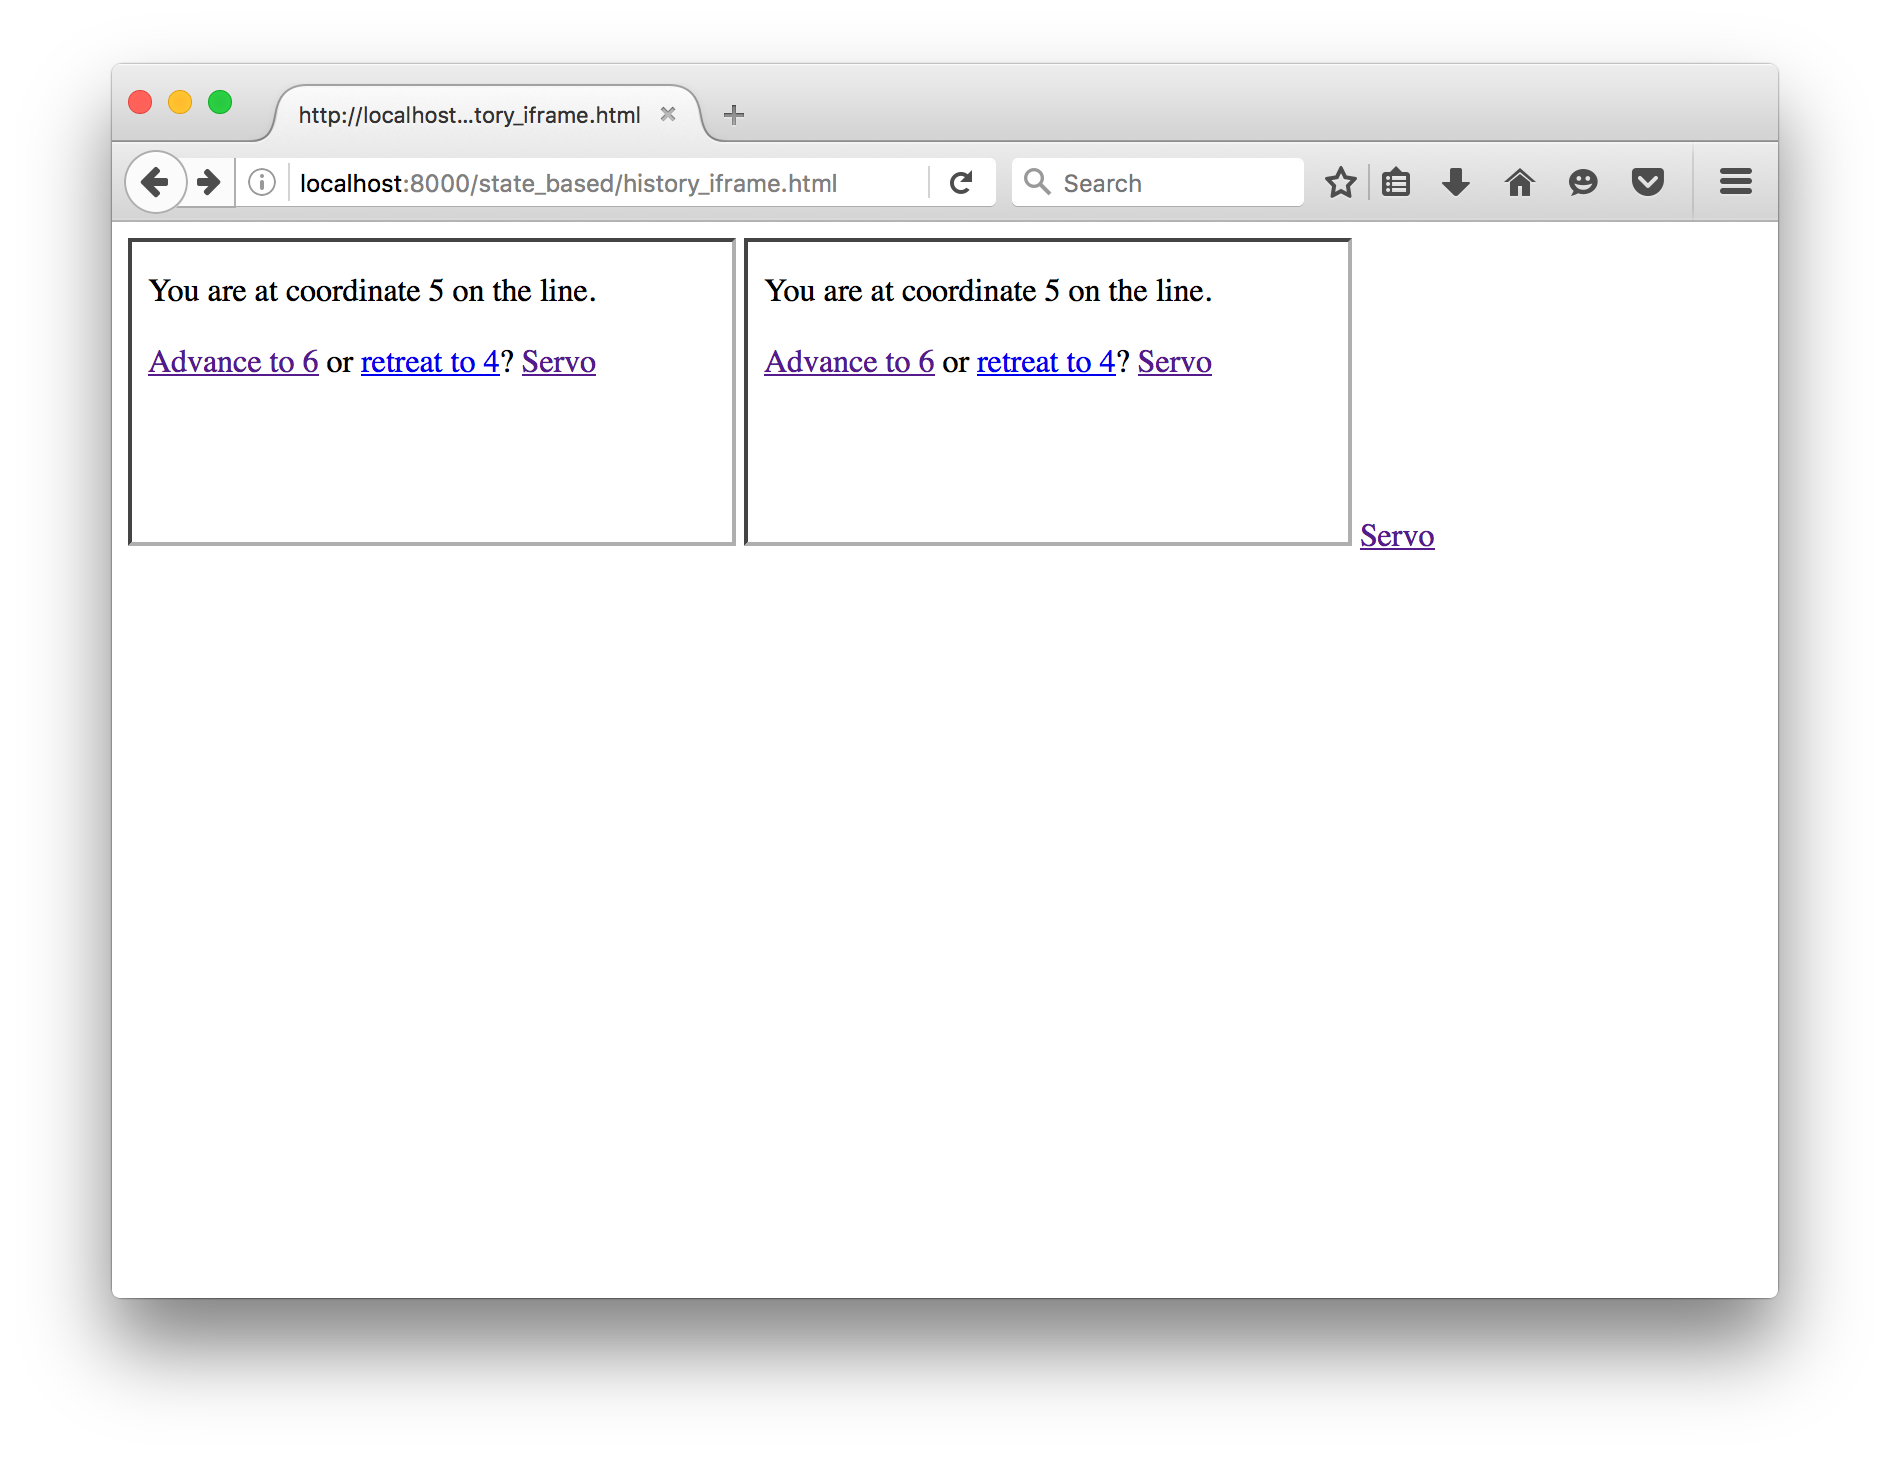
\includegraphics[width=.5\linewidth]{images/experiments/forwardback4state/firefox/6.png}%
    }~\raisebox{-.5\height}{
      \begin{tikzpicture}
        \node[doc,active,fully](0) at (0,0){0};
        \node[doc,active,fully](1) at (1,-1){1};
        \node[doc,jshactive,fully](2) at (2,-2){2};
        \node[doc](3) at (3,-1){3};
        \node[doc](4) at (4,-1){4};
        \node[doc](5) at (5,-2){5};
        \node[doc](6) at (6,-2){6};
        \node[draw,dotted,fit=(0)]{};
        \node[draw,dotted,fit=(1)(4)]{};
        \node[draw,dotted,fit=(2)(6)]{};
        \draw[->](0)--(1);
        \draw[->](0)to[out=-20,in=90](2);
      \end{tikzpicture}
    }
    \caption{Traverse $\aNH$ by $-4$}
  \end{figure}

  Traverse $\aNH$ by $4$:
  \begin{figure}[H]
    \raisebox{-.5\height}{
      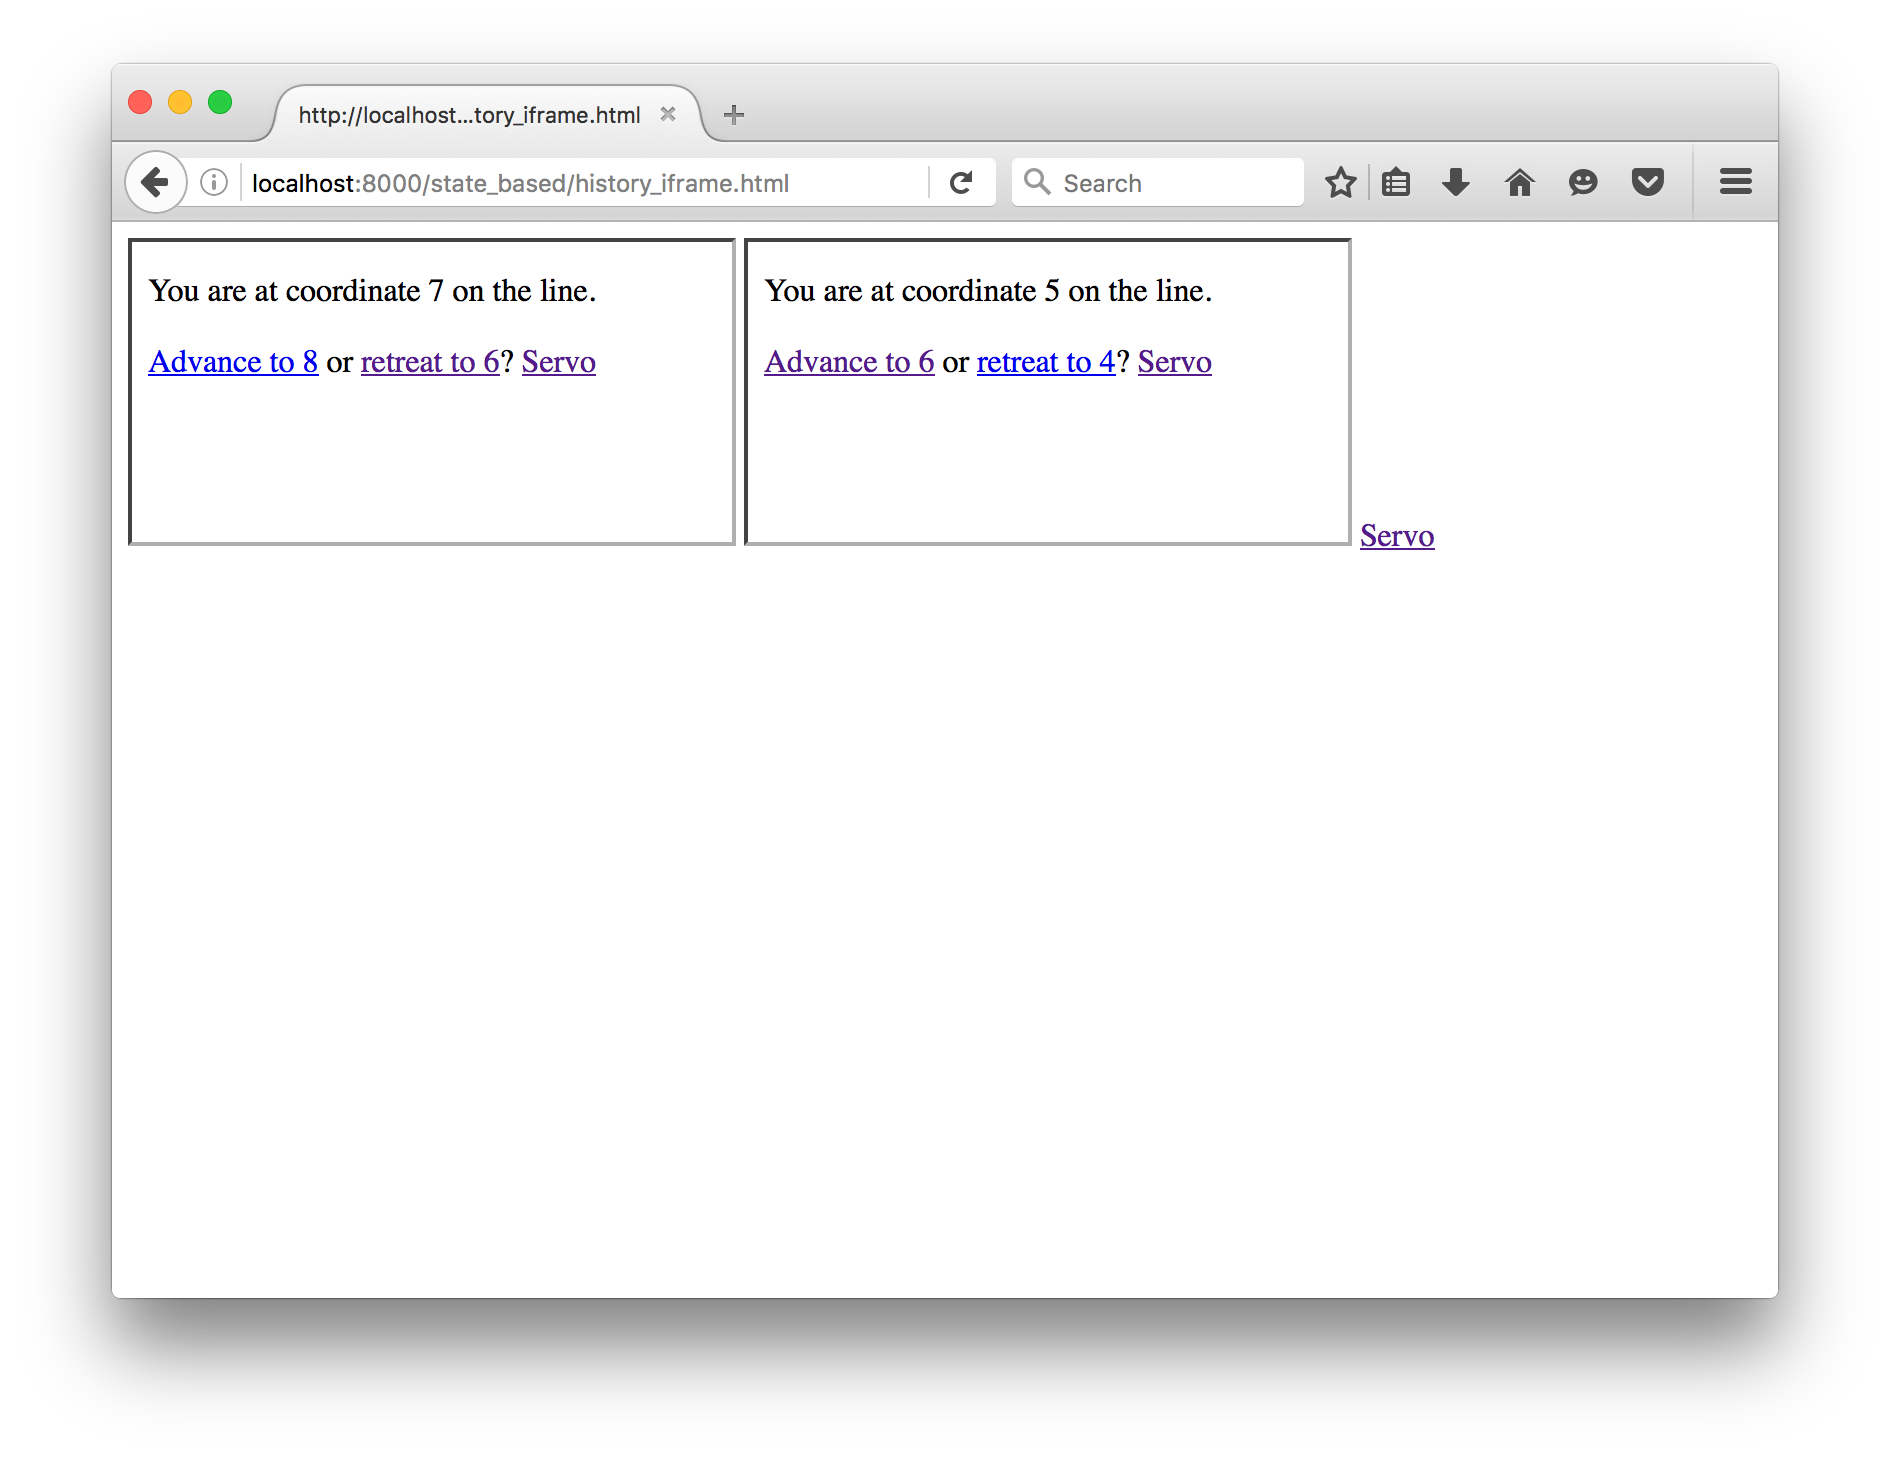
\includegraphics[width=.5\linewidth]{images/experiments/forwardback4state/firefox/7.png}%
    }~\raisebox{-.5\height}{
      \begin{tikzpicture}
        \node[doc,active,fully](0) at (0,0){0};
        \node[doc](1) at (1,-1){1};
        \node[doc,active,fully](2) at (2,-2){2};
        \node[doc](3) at (3,-1){3};
        \node[doc,jshactive,fully](4) at (4,-1){4};
        \node[doc](5) at (5,-2){5};
        \node[doc](6) at (6,-2){6};
        \node[draw,dotted,fit=(0)]{};
        \node[draw,dotted,fit=(1)(4)]{};
        \node[draw,dotted,fit=(2)(6)]{};
        \draw[->](0)to[out=0,in=140](4);
        \draw[->](0)to[out=-20,in=90](2);
      \end{tikzpicture}
    }
    \caption{Traverse $\aNH$ by $4$}
  \end{figure}

  The last traversal does not satisfy Goal~\ref{goal:homomorphism}.

  Safari:
  \begin{figure}[H]
    \raisebox{-.5\height}{
      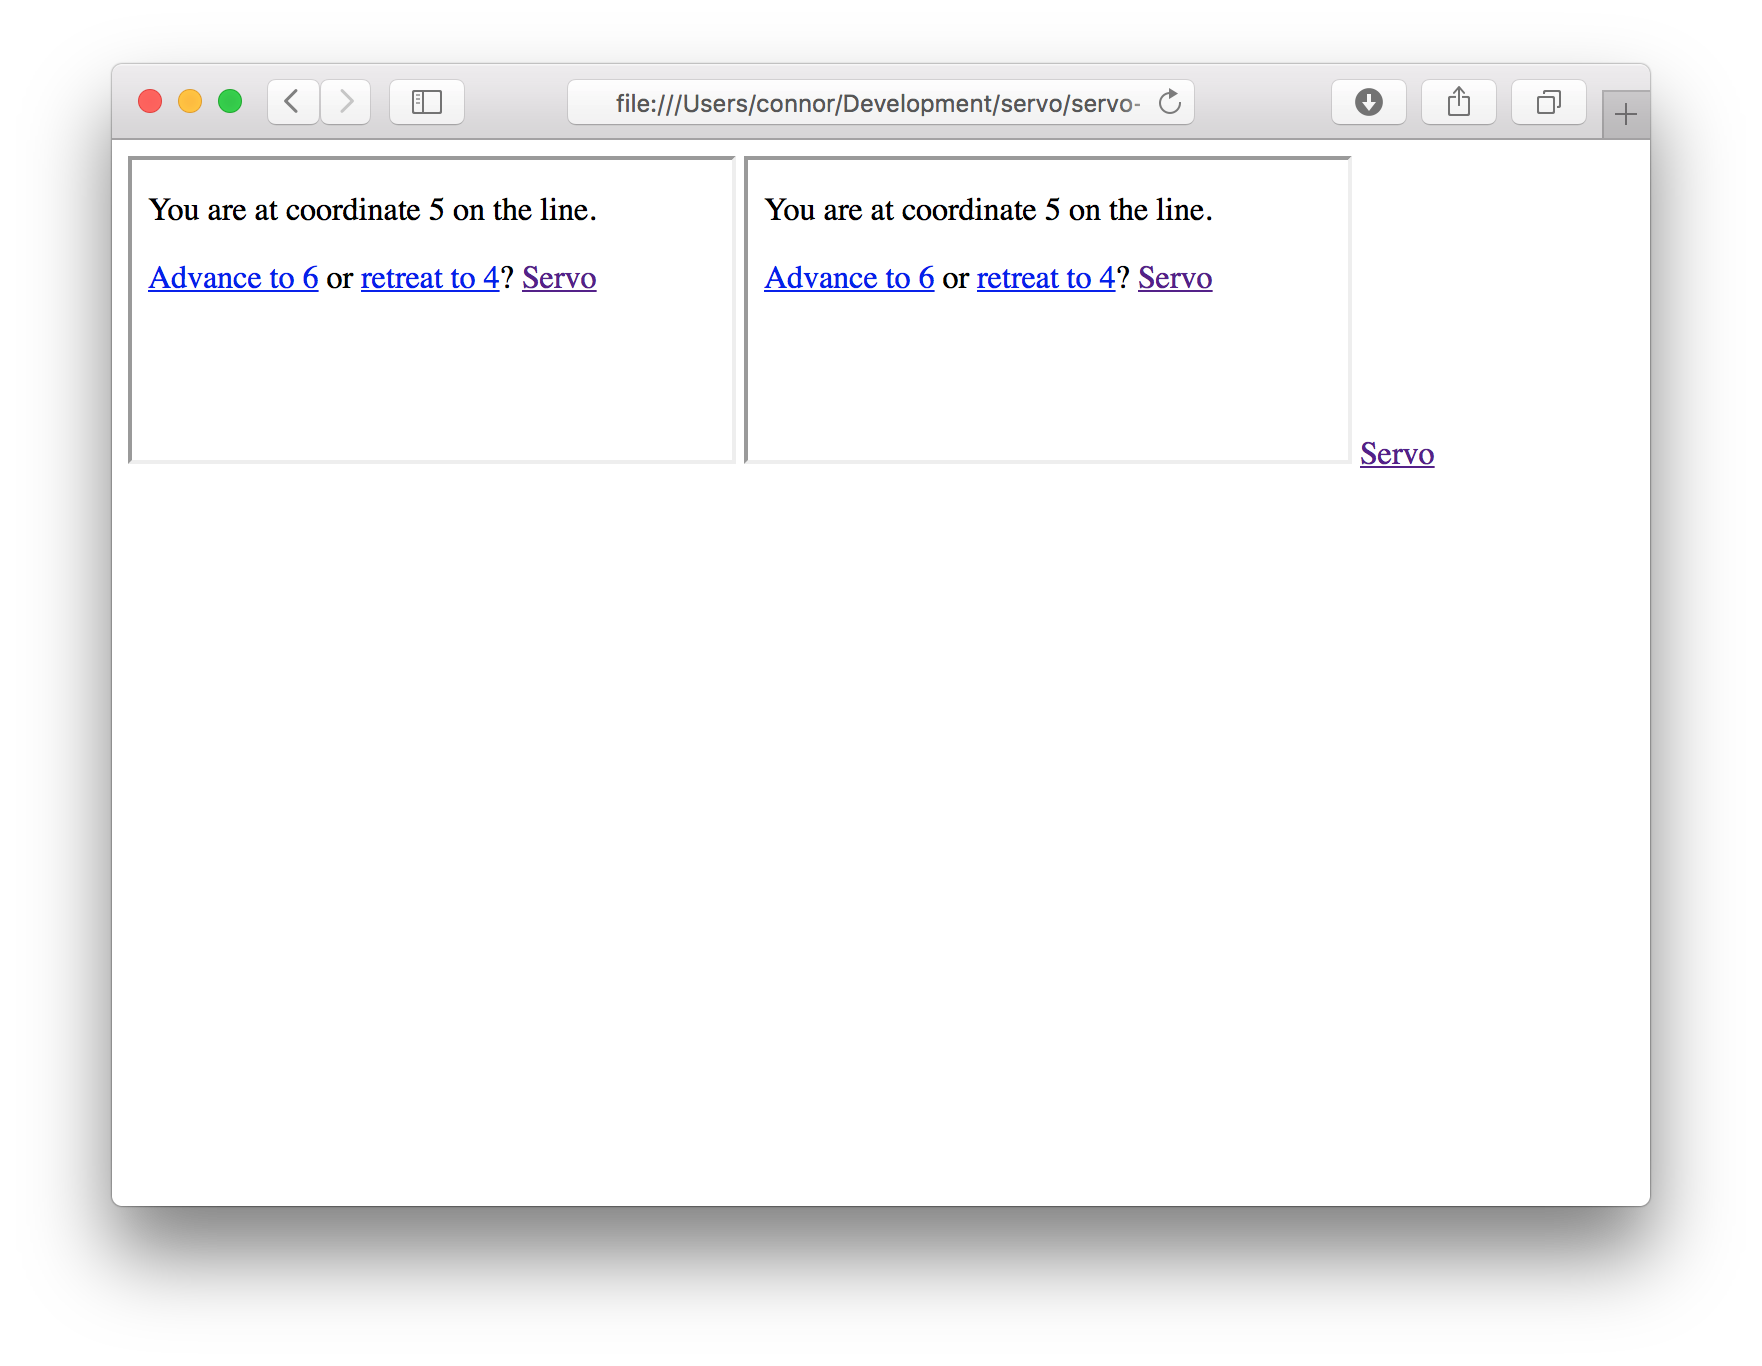
\includegraphics[width=.5\linewidth]{images/experiments/forwardback4state/safari/1.png}%
    }~\raisebox{-.5\height}{
      \begin{tikzpicture}
        \node[doc,active,fully](0) at (0,0){0};
        \node[doc,active,fully](1) at (1,-1){1};
        \node[doc,jshactive,fully](2) at (2,-2){2};
        \node[draw,dotted,fit=(0)]{};
        \node[draw,dotted,fit=(1)]{};
        \node[draw,dotted,fit=(2)]{};
        \draw[->](0)--(1);
        \draw[->](0)to[out=-20,in=90](2);
      \end{tikzpicture}
    }
    \caption{Initial State}
  \end{figure}

  Advance document 1 to $6$:
  \begin{figure}[H]
    \raisebox{-.5\height}{
      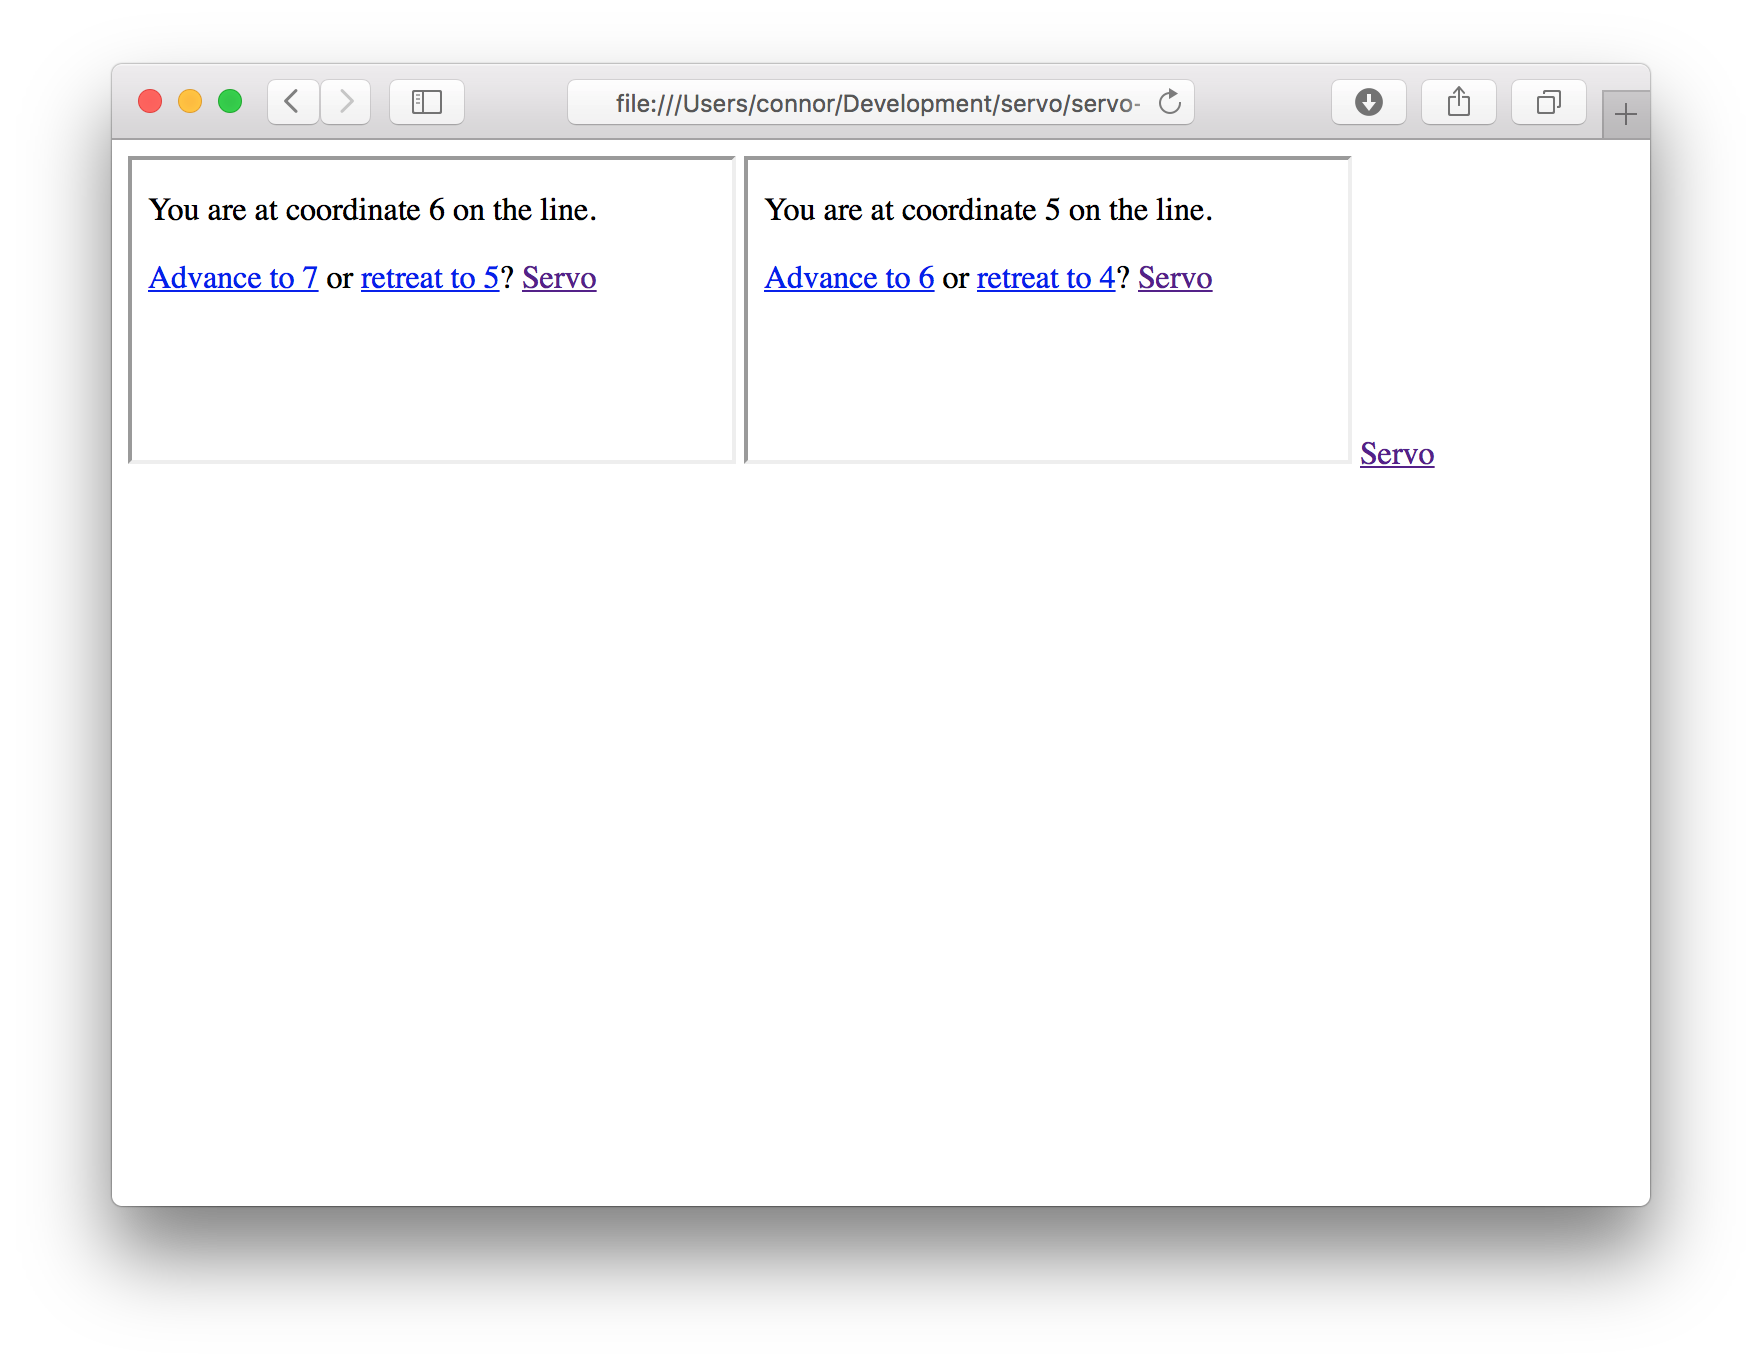
\includegraphics[width=.5\linewidth]{images/experiments/forwardback4state/safari/2.png}%
    }~\raisebox{-.5\height}{
      \begin{tikzpicture}
        \node[doc,active,fully](0) at (0,0){0};
        \node[doc](1) at (1,-1){1};
        \node[doc,active,fully](2) at (2,-2){2};
        \node[doc,jshactive,fully](3) at (3,-1){3};
        \node[draw,dotted,fit=(0)]{};
        \node[draw,dotted,fit=(1)(3)]{};
        \node[draw,dotted,fit=(2)]{};
        \draw[->](0)--(3);
        \draw[->](0)to[out=-20,in=90](2);
      \end{tikzpicture}
    }
    \caption{Advance document 1 to $6$}
  \end{figure}

  Advance document 3 to $7$:
  \begin{figure}[H]
    \raisebox{-.5\height}{
      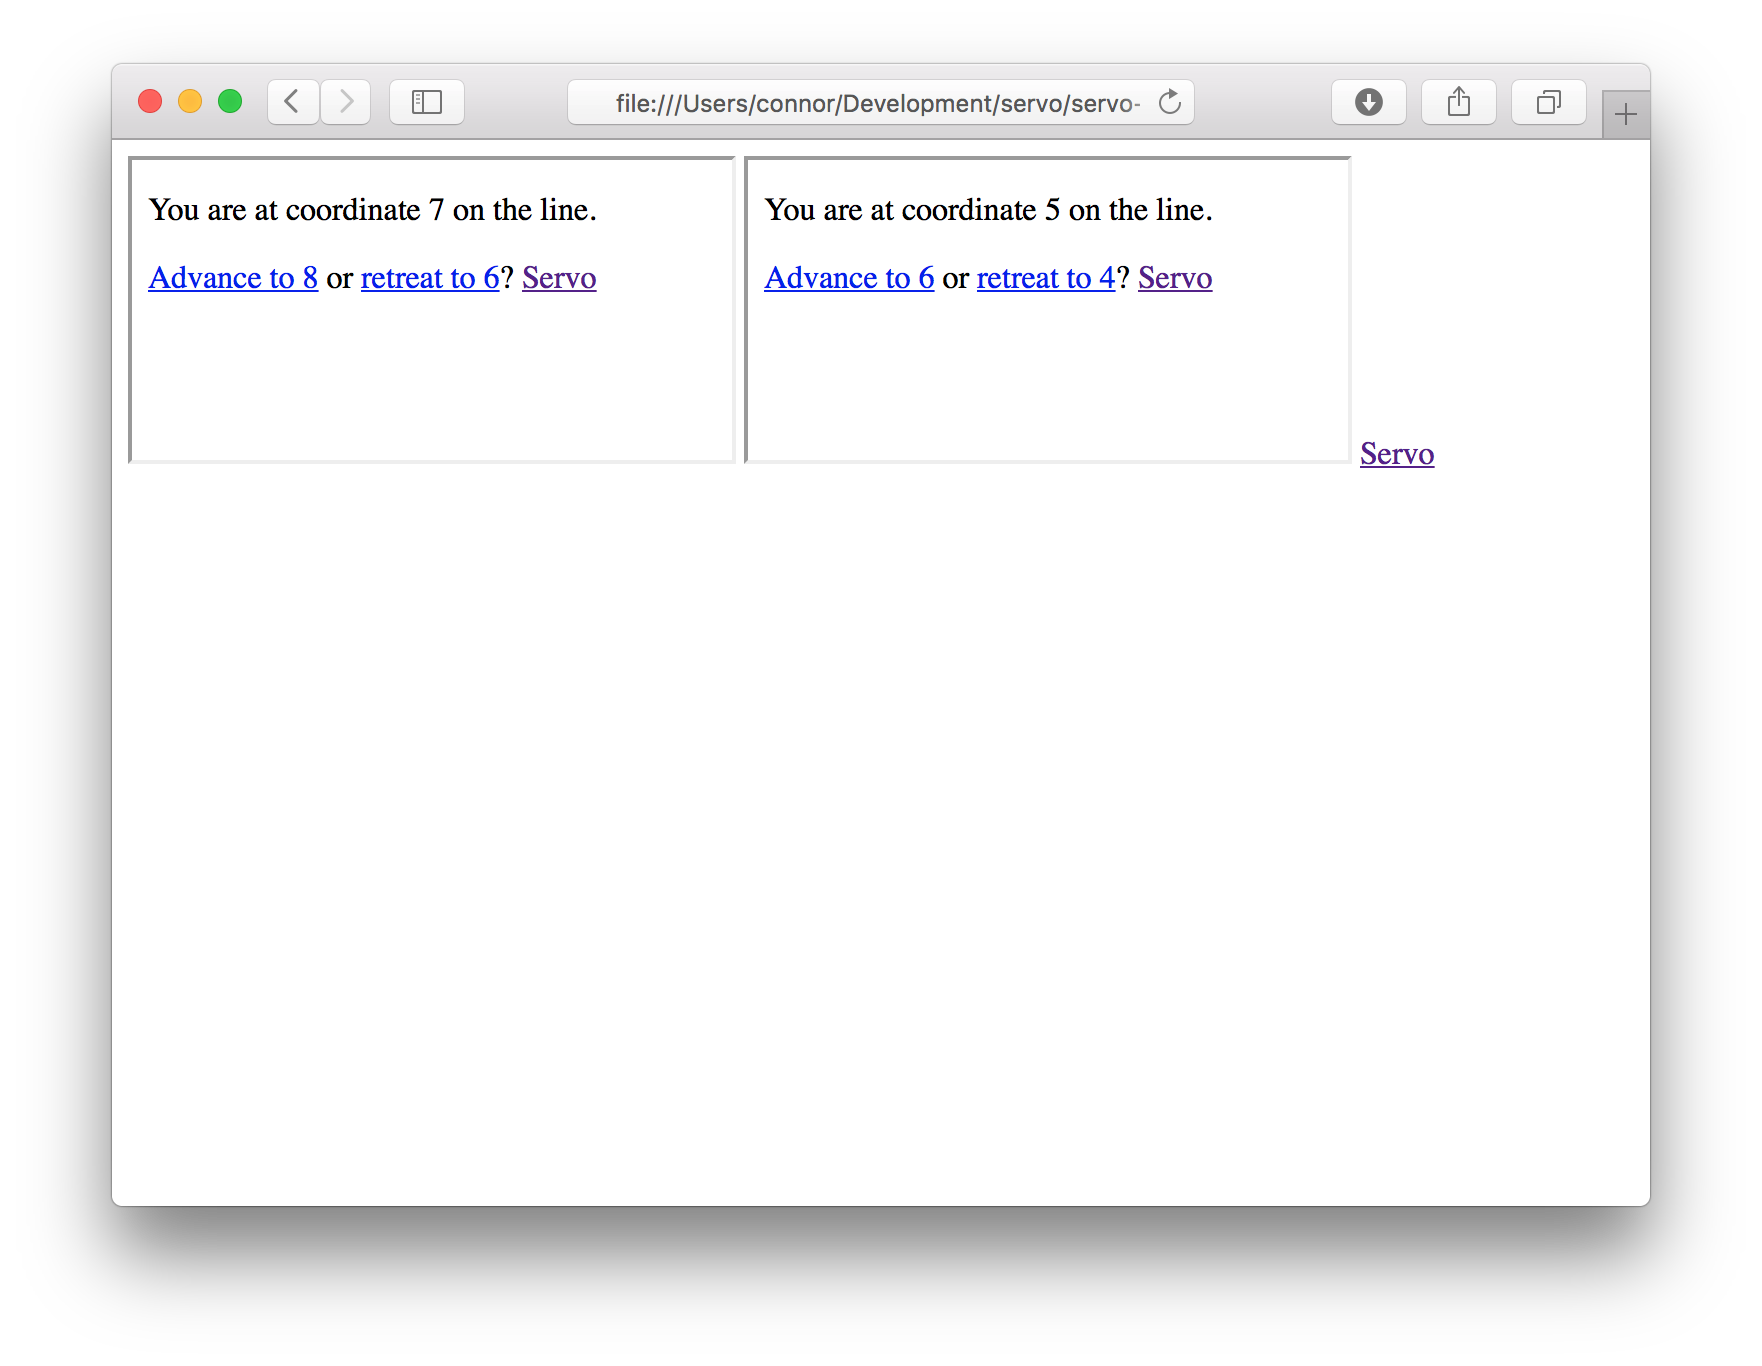
\includegraphics[width=.5\linewidth]{images/experiments/forwardback4state/safari/3.png}%
    }~\raisebox{-.5\height}{
      \begin{tikzpicture}
        \node[doc,active,fully](0) at (0,0){0};
        \node[doc](1) at (1,-1){1};
        \node[doc,active,fully](2) at (2,-2){2};
        \node[doc](3) at (3,-1){3};
        \node[doc,jshactive,fully](4) at (4,-1){4};
        \node[draw,dotted,fit=(0)]{};
        \node[draw,dotted,fit=(1)(4)]{};
        \node[draw,dotted,fit=(2)]{};
        \draw[->](0)to[out=0,in=140](4);
        \draw[->](0)to[out=-20,in=90](2);
      \end{tikzpicture}
    }
    \caption{Advance document 3 to $7$}
  \end{figure}

  Advance document 2 to $6$:
  \begin{figure}[H]
    \raisebox{-.5\height}{
      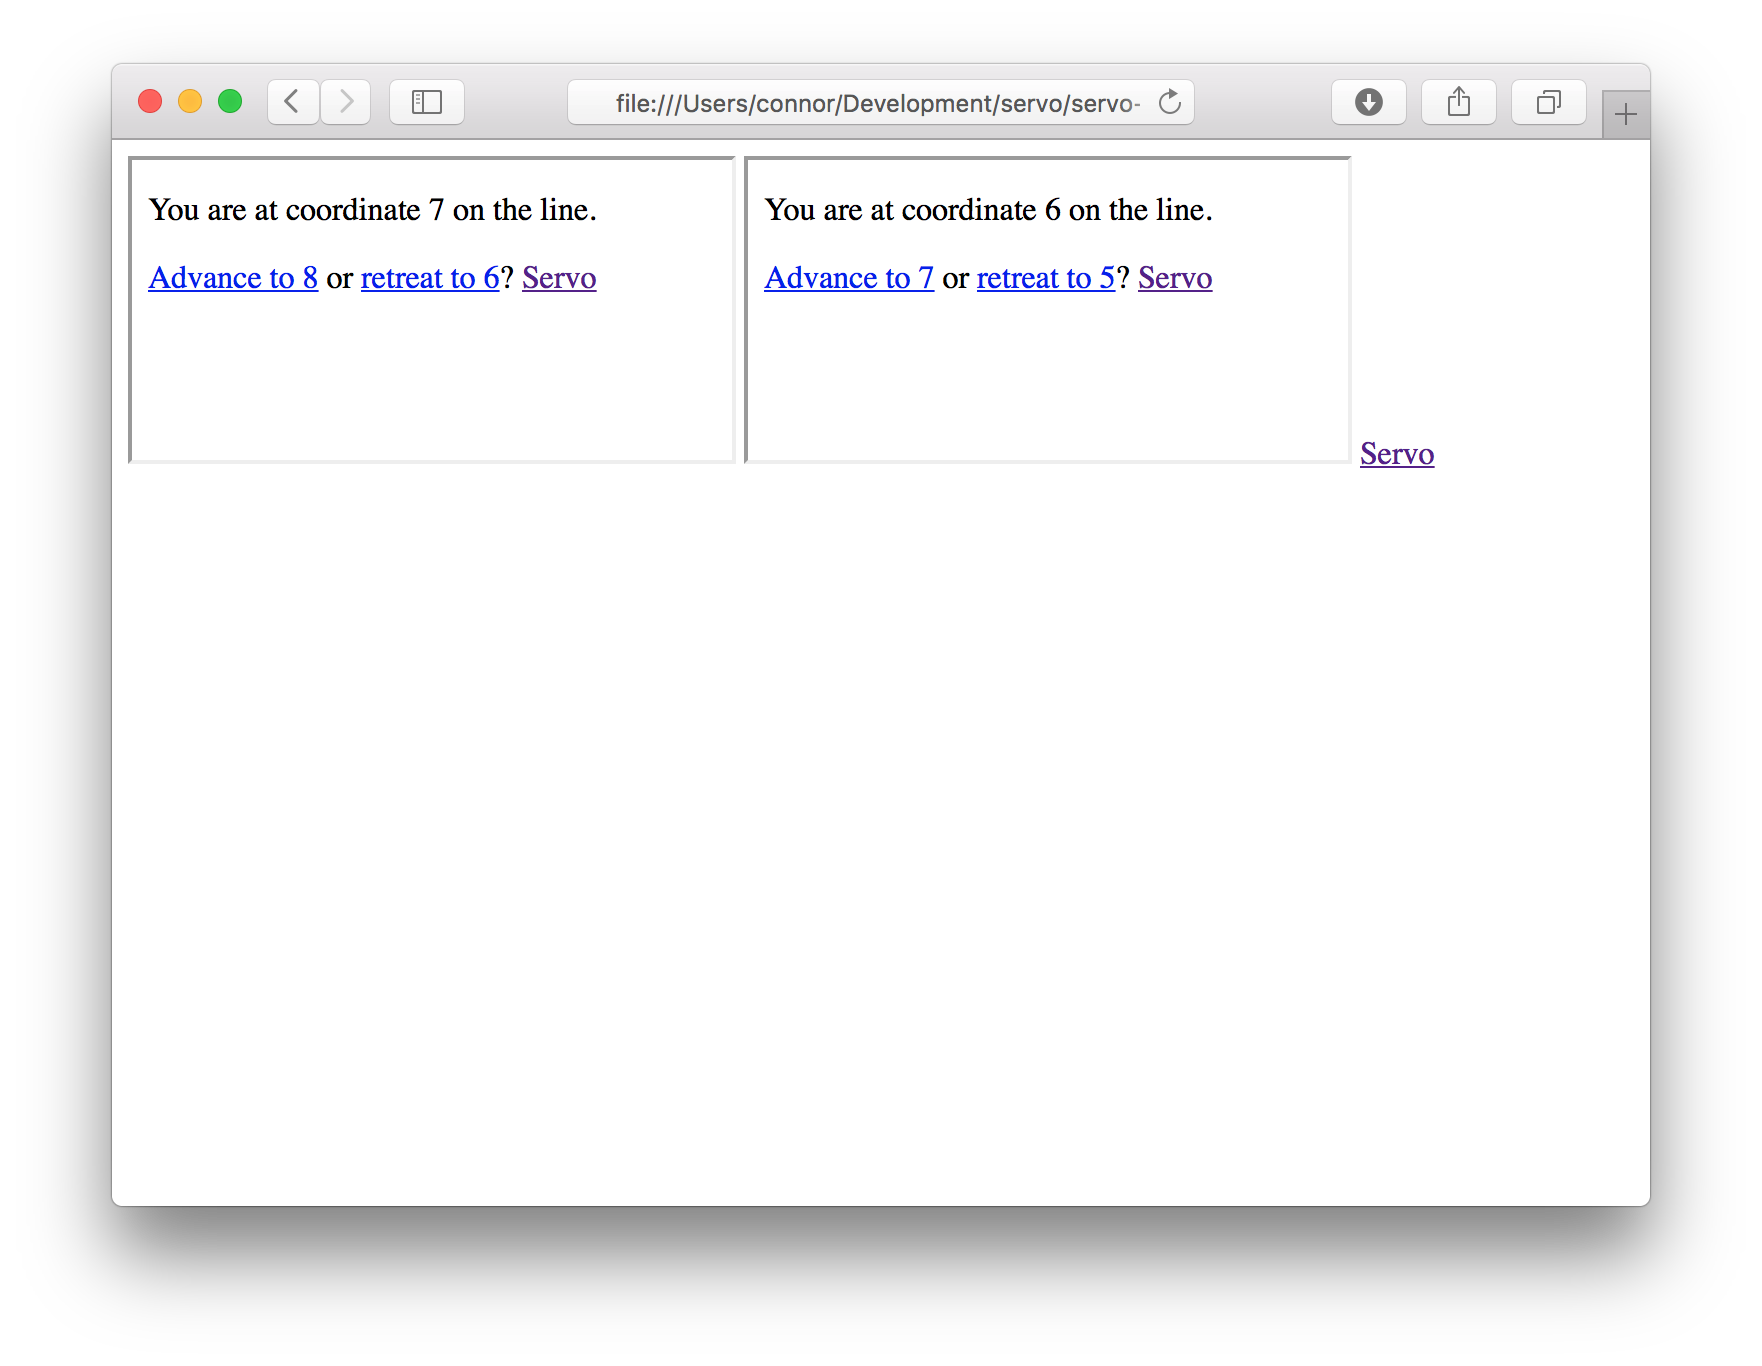
\includegraphics[width=.5\linewidth]{images/experiments/forwardback4state/safari/4.png}%
    }~\raisebox{-.5\height}{
      \begin{tikzpicture}
        \node[doc,active,fully](0) at (0,0){0};
        \node[doc](1) at (1,-1){1};
        \node[doc](2) at (2,-2){2};
        \node[doc](3) at (3,-1){3};
        \node[doc,active,fully](4) at (4,-1){4};
        \node[doc,jshactive,fully](5) at (5,-2){5};
        \node[draw,dotted,fit=(0)]{};
        \node[draw,dotted,fit=(1)(4)]{};
        \node[draw,dotted,fit=(2)(5)]{};
        \draw[->](0)to[out=0,in=140](4);
        \draw[->](0)to[out=0,in=90](5);
      \end{tikzpicture}
    }
    \caption{Advance document $2$ to $6$}
  \end{figure}

  Advance $document 2$ to $7$:
  \begin{figure}[H]
    \raisebox{-.5\height}{
      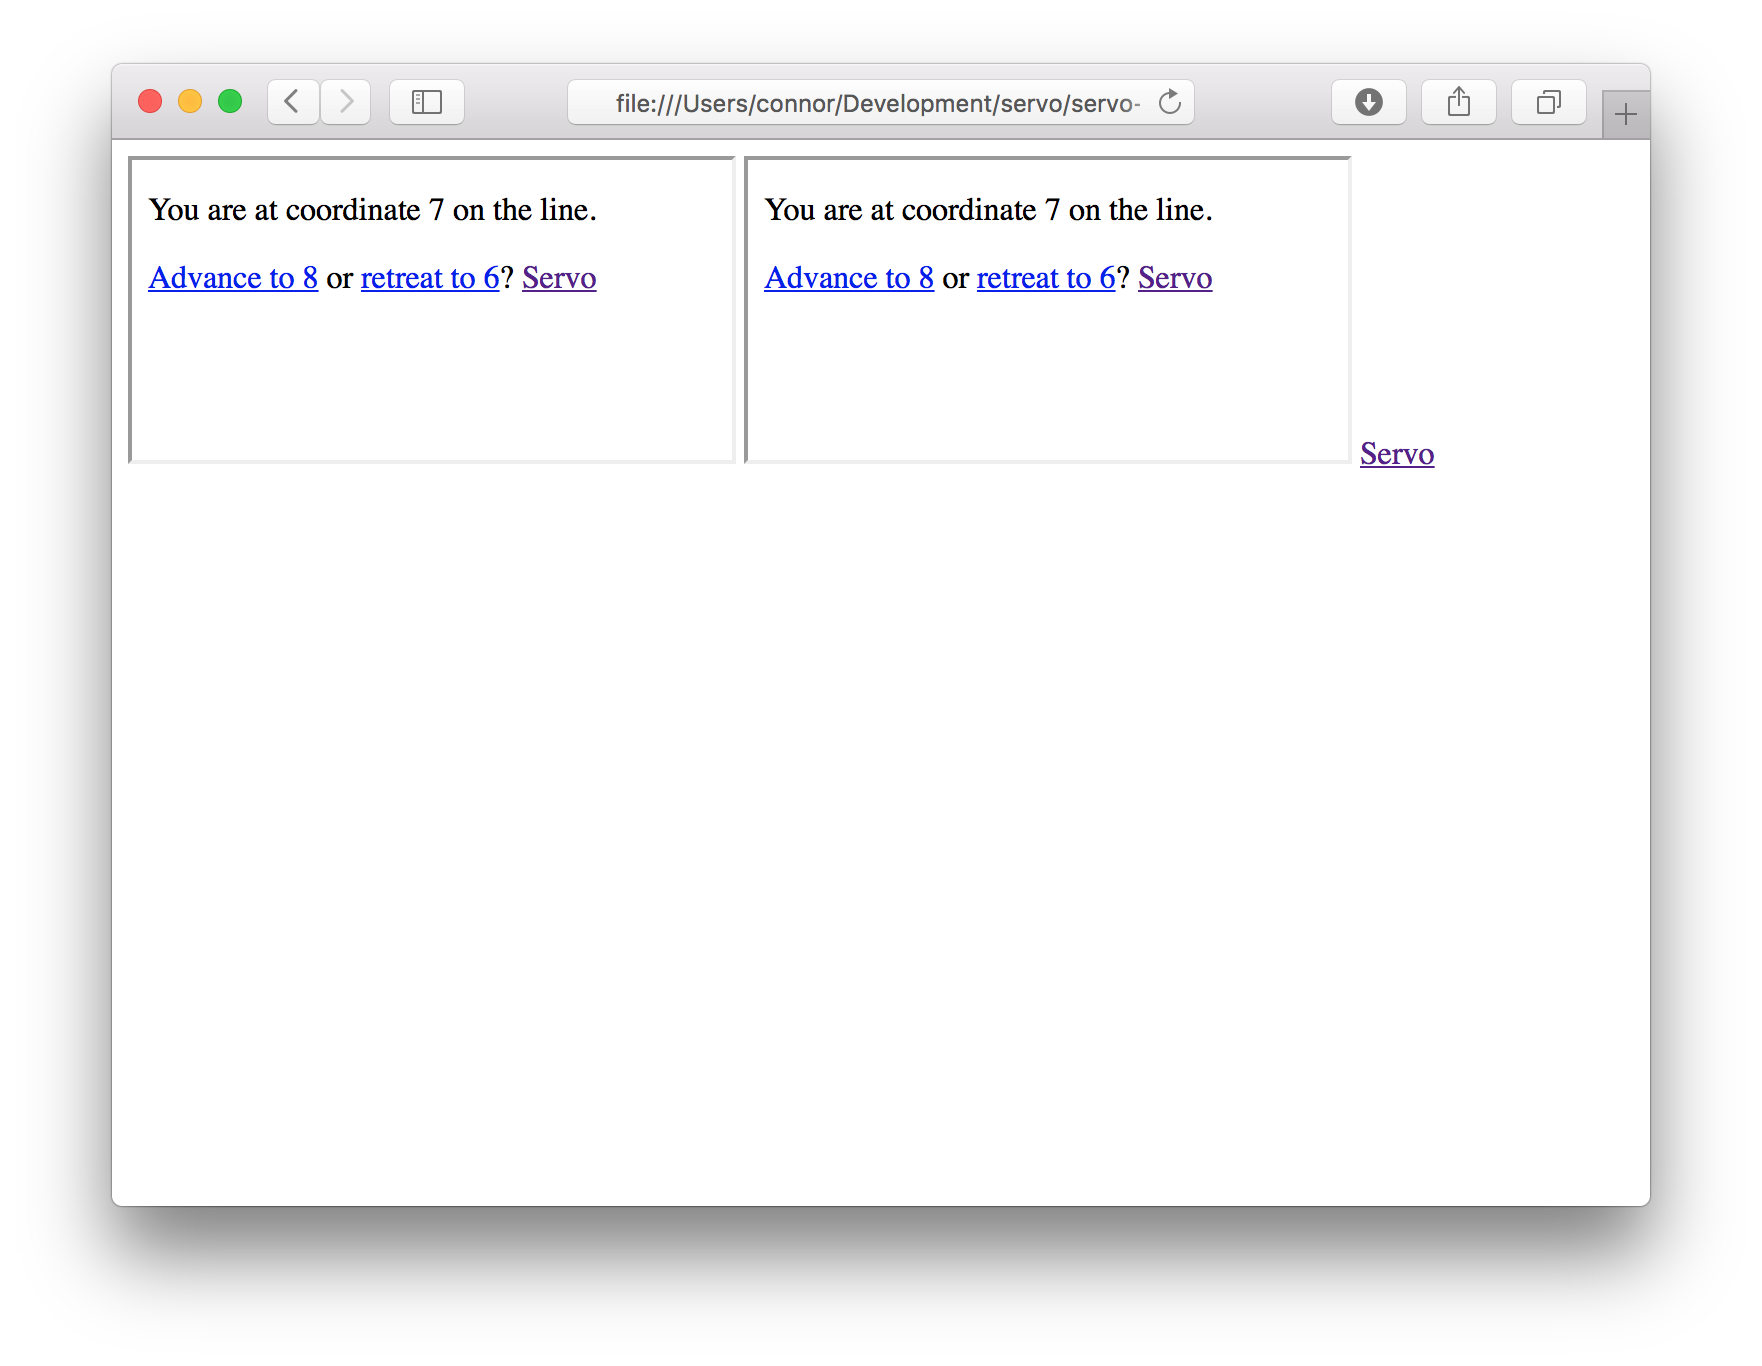
\includegraphics[width=.5\linewidth]{images/experiments/forwardback4state/safari/5.png}%
    }~\raisebox{-.5\height}{
      \begin{tikzpicture}
        \node[doc,active,fully](0) at (0,0){0};
        \node[doc](1) at (1,-1){1};
        \node[doc](2) at (2,-2){2};
        \node[doc](3) at (3,-1){3};
        \node[doc,active,fully](4) at (4,-1){4};
        \node[doc](5) at (5,-2){5};
        \node[doc,jshactive,fully](6) at (6,-2){6};
        \node[draw,dotted,fit=(0)]{};
        \node[draw,dotted,fit=(1)(4)]{};
        \node[draw,dotted,fit=(2)(6)]{};
        \draw[->](0)to[out=0,in=140](4);
        \draw[->](0)to[out=0,in=120](6);
      \end{tikzpicture}
    }
    \caption{Advance document 2 to $7$}
  \end{figure}

  Traverse $\aNH$ by $-4$:
  \begin{figure}[H]
    \raisebox{-.5\height}{
      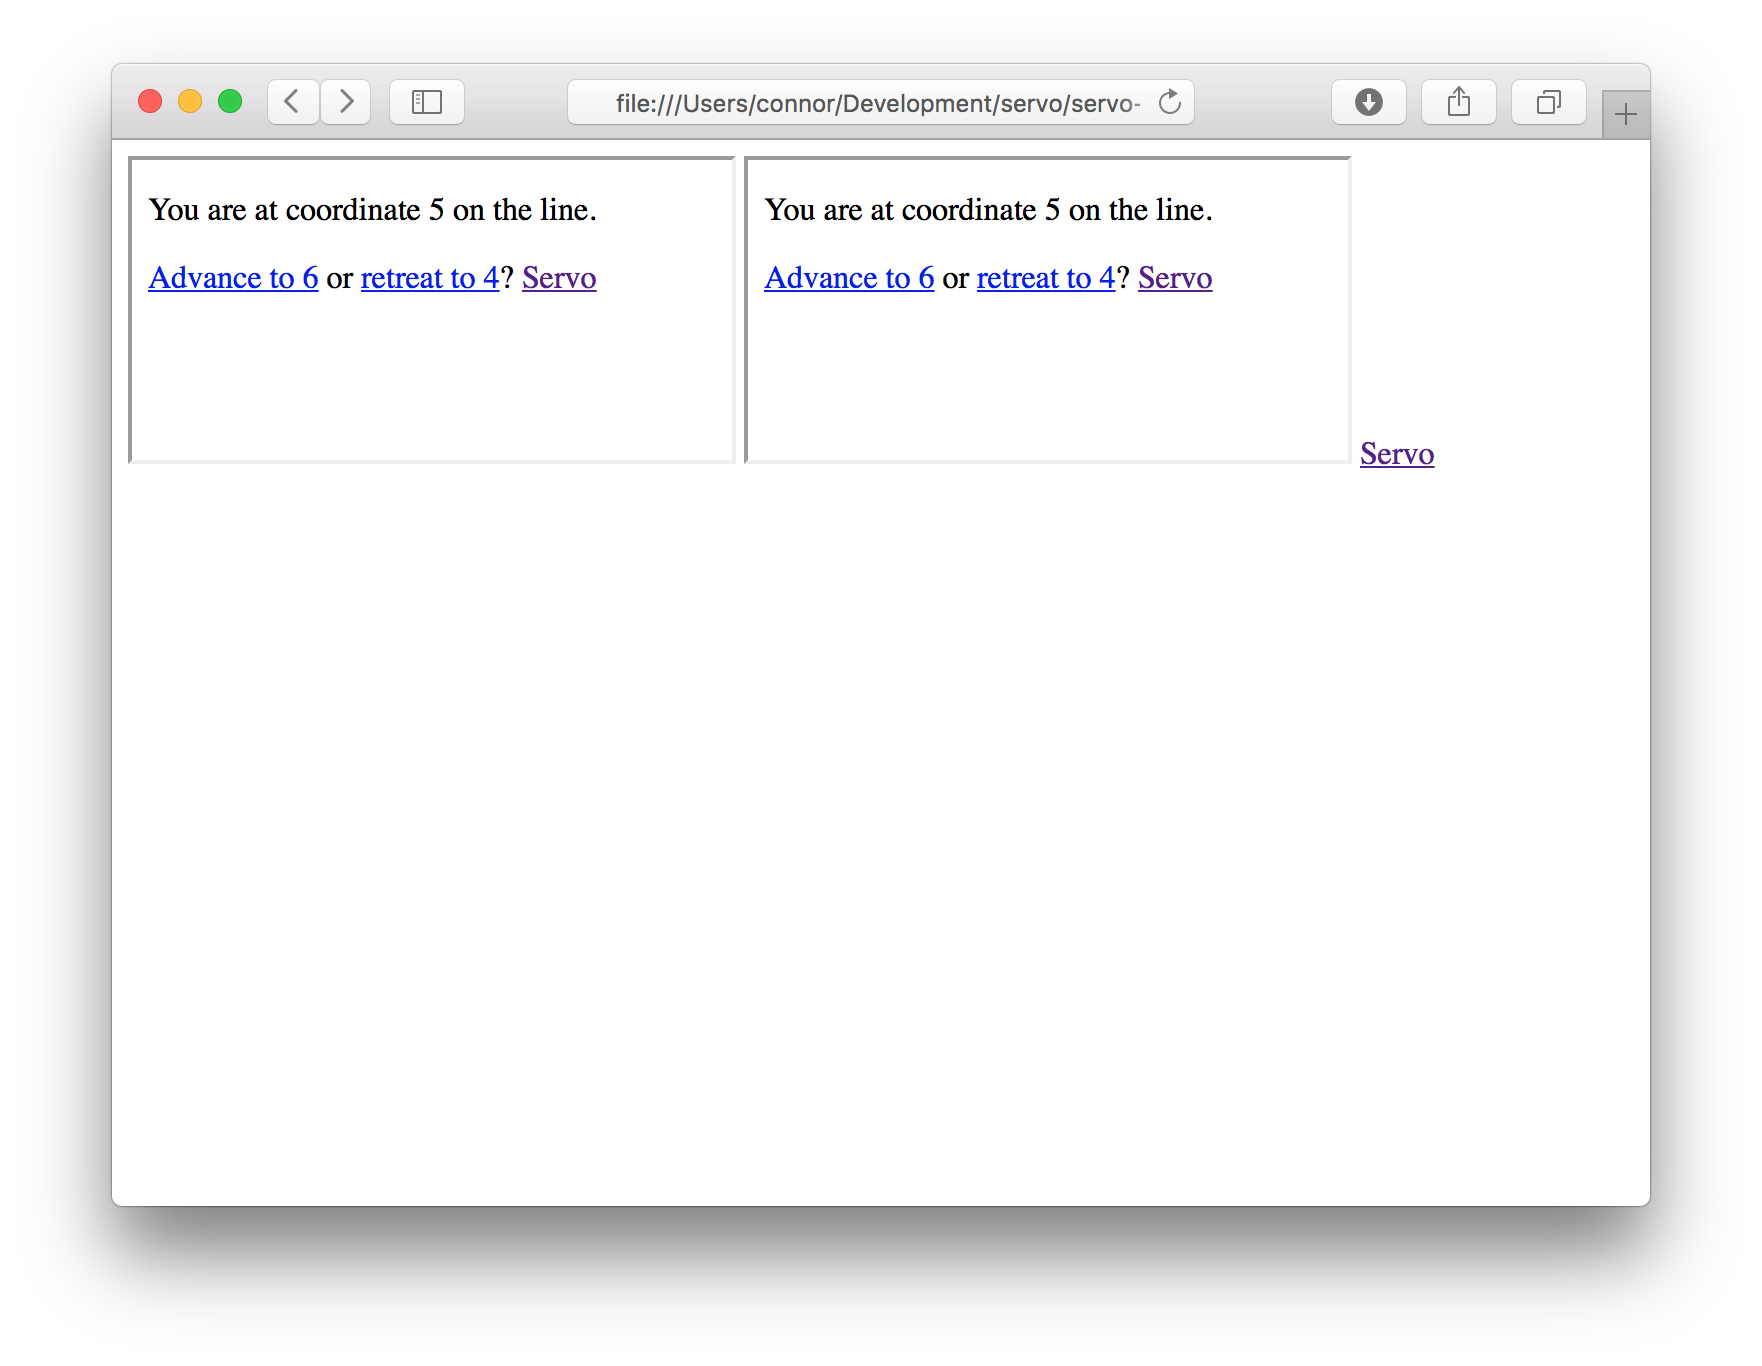
\includegraphics[width=.5\linewidth]{images/experiments/forwardback4state/safari/6.png}%
    }~\raisebox{-.5\height}{
      \begin{tikzpicture}
        \node[doc,active,fully](0) at (0,0){0};
        \node[doc,active,fully](1) at (1,-1){1};
        \node[doc,jshactive,fully](2) at (2,-2){2};
        \node[doc](3) at (3,-1){3};
        \node[doc](4) at (4,-1){4};
        \node[doc](5) at (5,-2){5};
        \node[doc](6) at (6,-2){6};
        \node[draw,dotted,fit=(0)]{};
        \node[draw,dotted,fit=(1)(4)]{};
        \node[draw,dotted,fit=(2)(6)]{};
        \draw[->](0)--(1);
        \draw[->](0)to[out=-20,in=90](2);
      \end{tikzpicture}
    }
    \caption{Traverse $\aNH$ by $-4$}
  \end{figure}

  Traverse $\aNH$ by $4$:
  \begin{figure}[H]
    \raisebox{-.5\height}{
      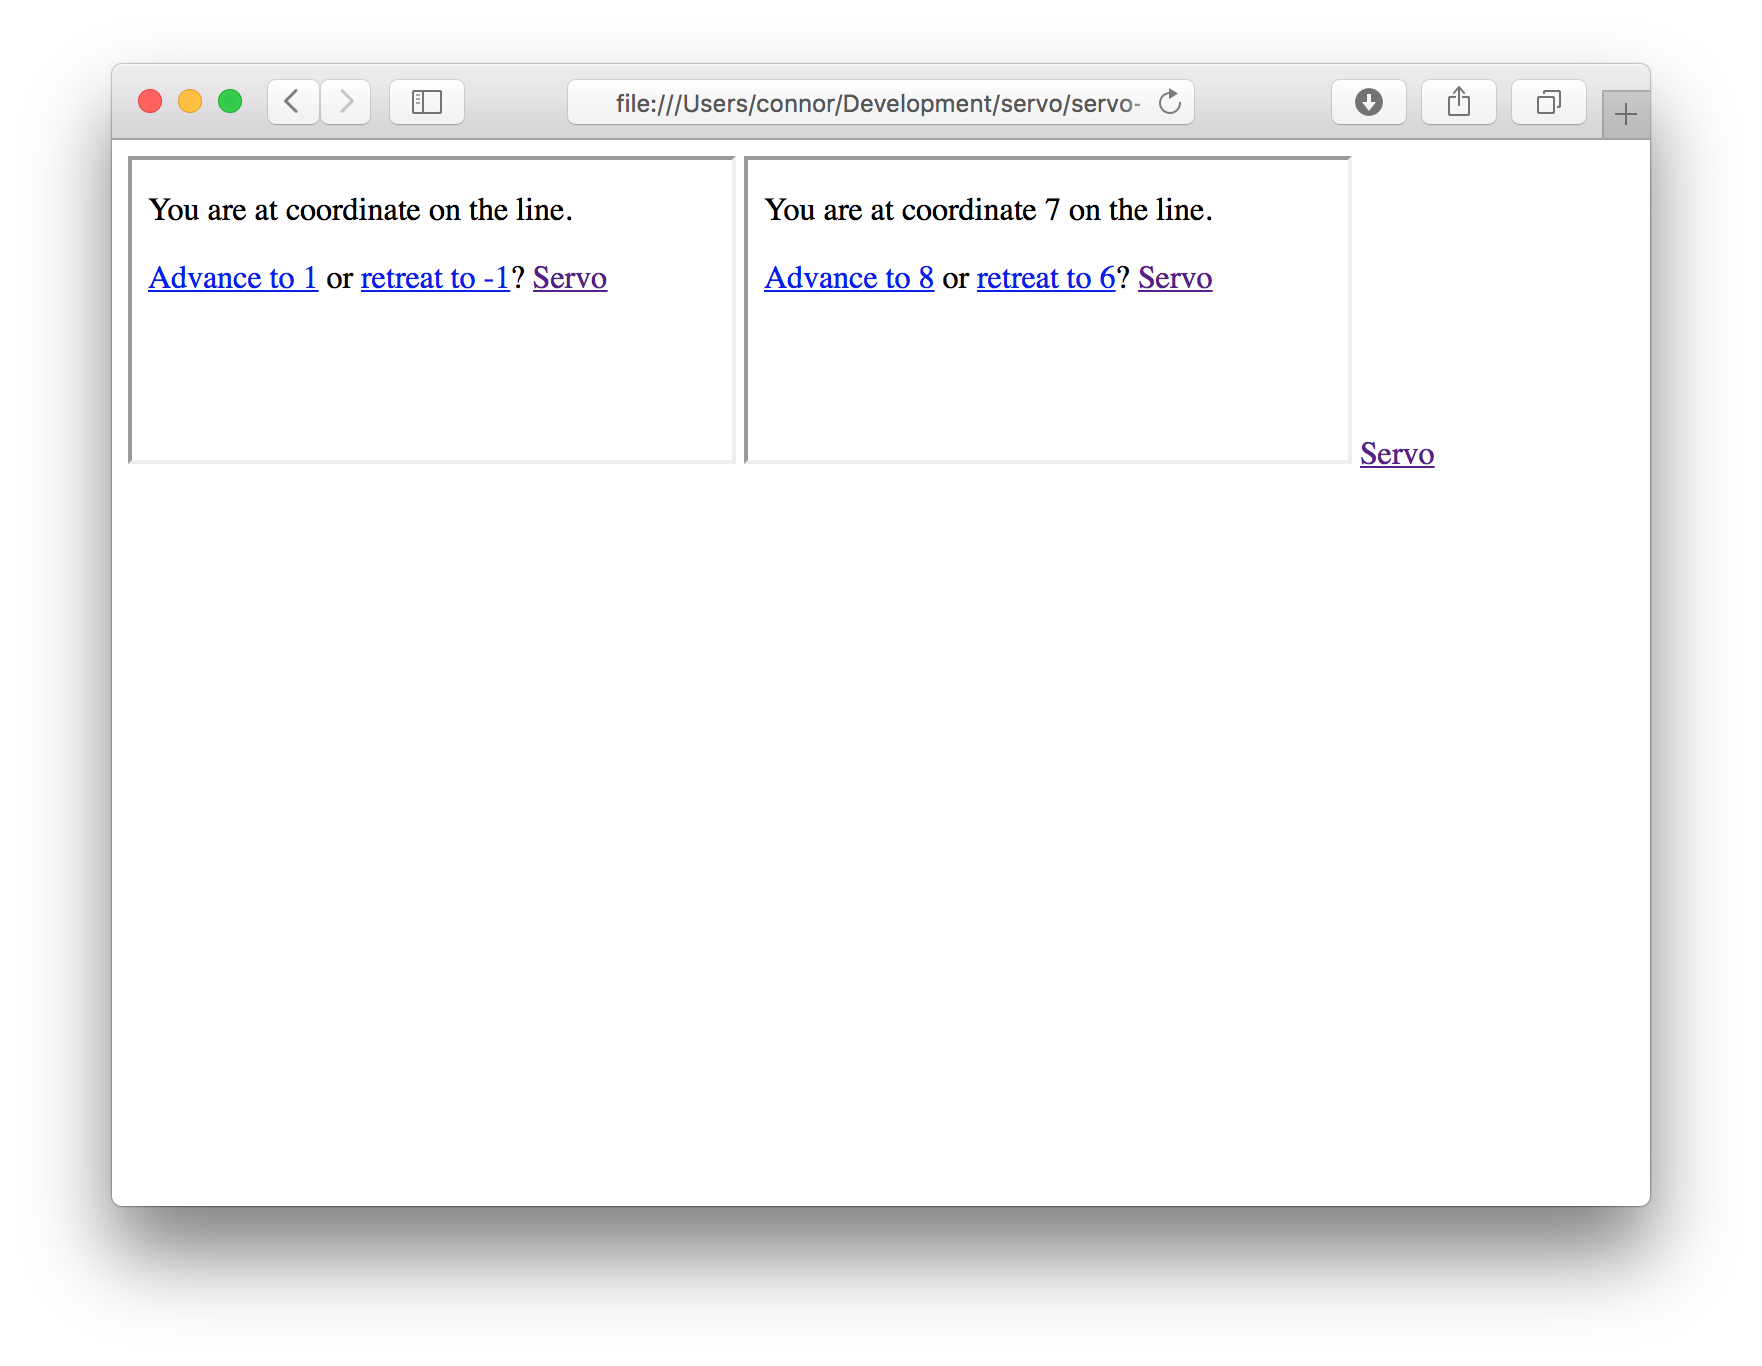
\includegraphics[width=.5\linewidth]{images/experiments/forwardback4state/safari/7.png}%
    }~\raisebox{-.5\height}{
      \begin{tikzpicture}
        \node[doc,active,fully](0) at (0,0){0};
        \node[doc](1) at (1,-1){1};
        \node[doc](2) at (2,-2){2};
        \node[doc](3) at (3,-1){3};
        \node[doc,jshactive,fully](4) at (4,-1){4};
        \node[doc](5) at (5,-2){5};
        \node[doc](6) at (6,-2){6};
        \node[draw,dotted,fit=(0)]{};
        \node[draw,dotted,fit=(1)(4)]{};
        \node[draw,dotted,fit=(2)(6)]{};
        \draw[->](0)to[out=0,in=140](4);
      \end{tikzpicture}
    }
    \caption{Traverse $\aNH$ by $4$}
  \end{figure}

  In this traversal, we are unable to determine the active entry for first entry as the state is $null$.
  This traversal does not satisfy Goal~\ref{goal:homomorphism}.

  Chrome:
  \begin{figure}[H]
    \raisebox{-.5\height}{
      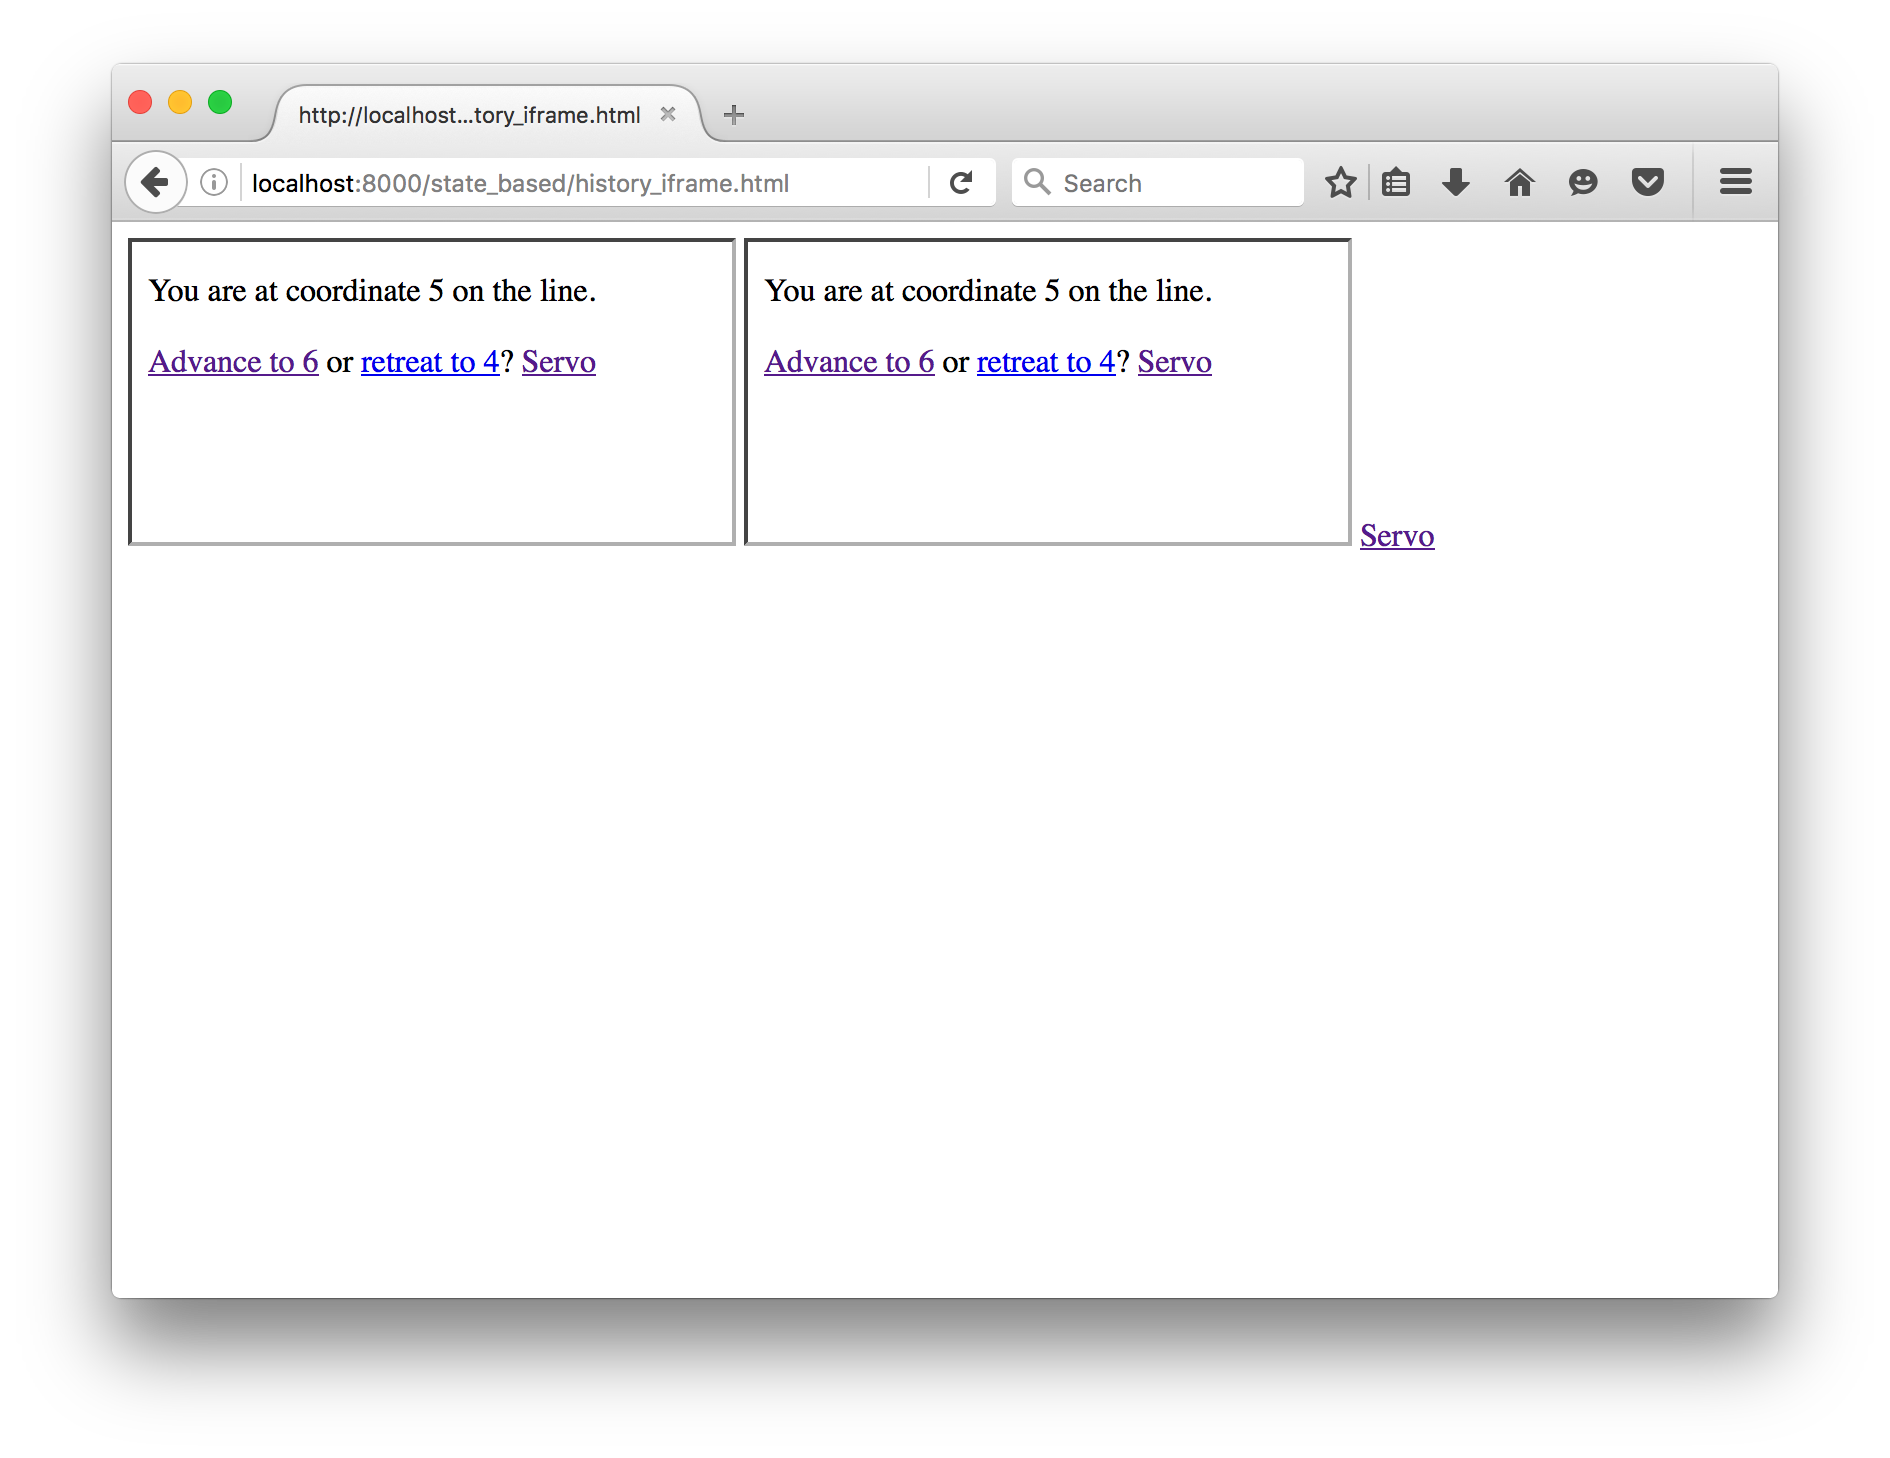
\includegraphics[width=.5\linewidth]{images/experiments/forwardback4state/firefox/1.png}%
    }~\raisebox{-.5\height}{
      \begin{tikzpicture}
        \node[doc,active,fully](0) at (0,0){0};
        \node[doc,active,fully](1) at (1,-1){1};
        \node[doc,jshactive,fully](2) at (2,-2){2};
        \node[draw,dotted,fit=(0)]{};
        \node[draw,dotted,fit=(1)]{};
        \node[draw,dotted,fit=(2)]{};
        \draw[->](0)--(1);
        \draw[->](0)to[out=-20,in=90](2);
      \end{tikzpicture}
    }
    \caption{Initial State}
  \end{figure}

  Advance document 1 to $6$:
  \begin{figure}[H]
    \raisebox{-.5\height}{
      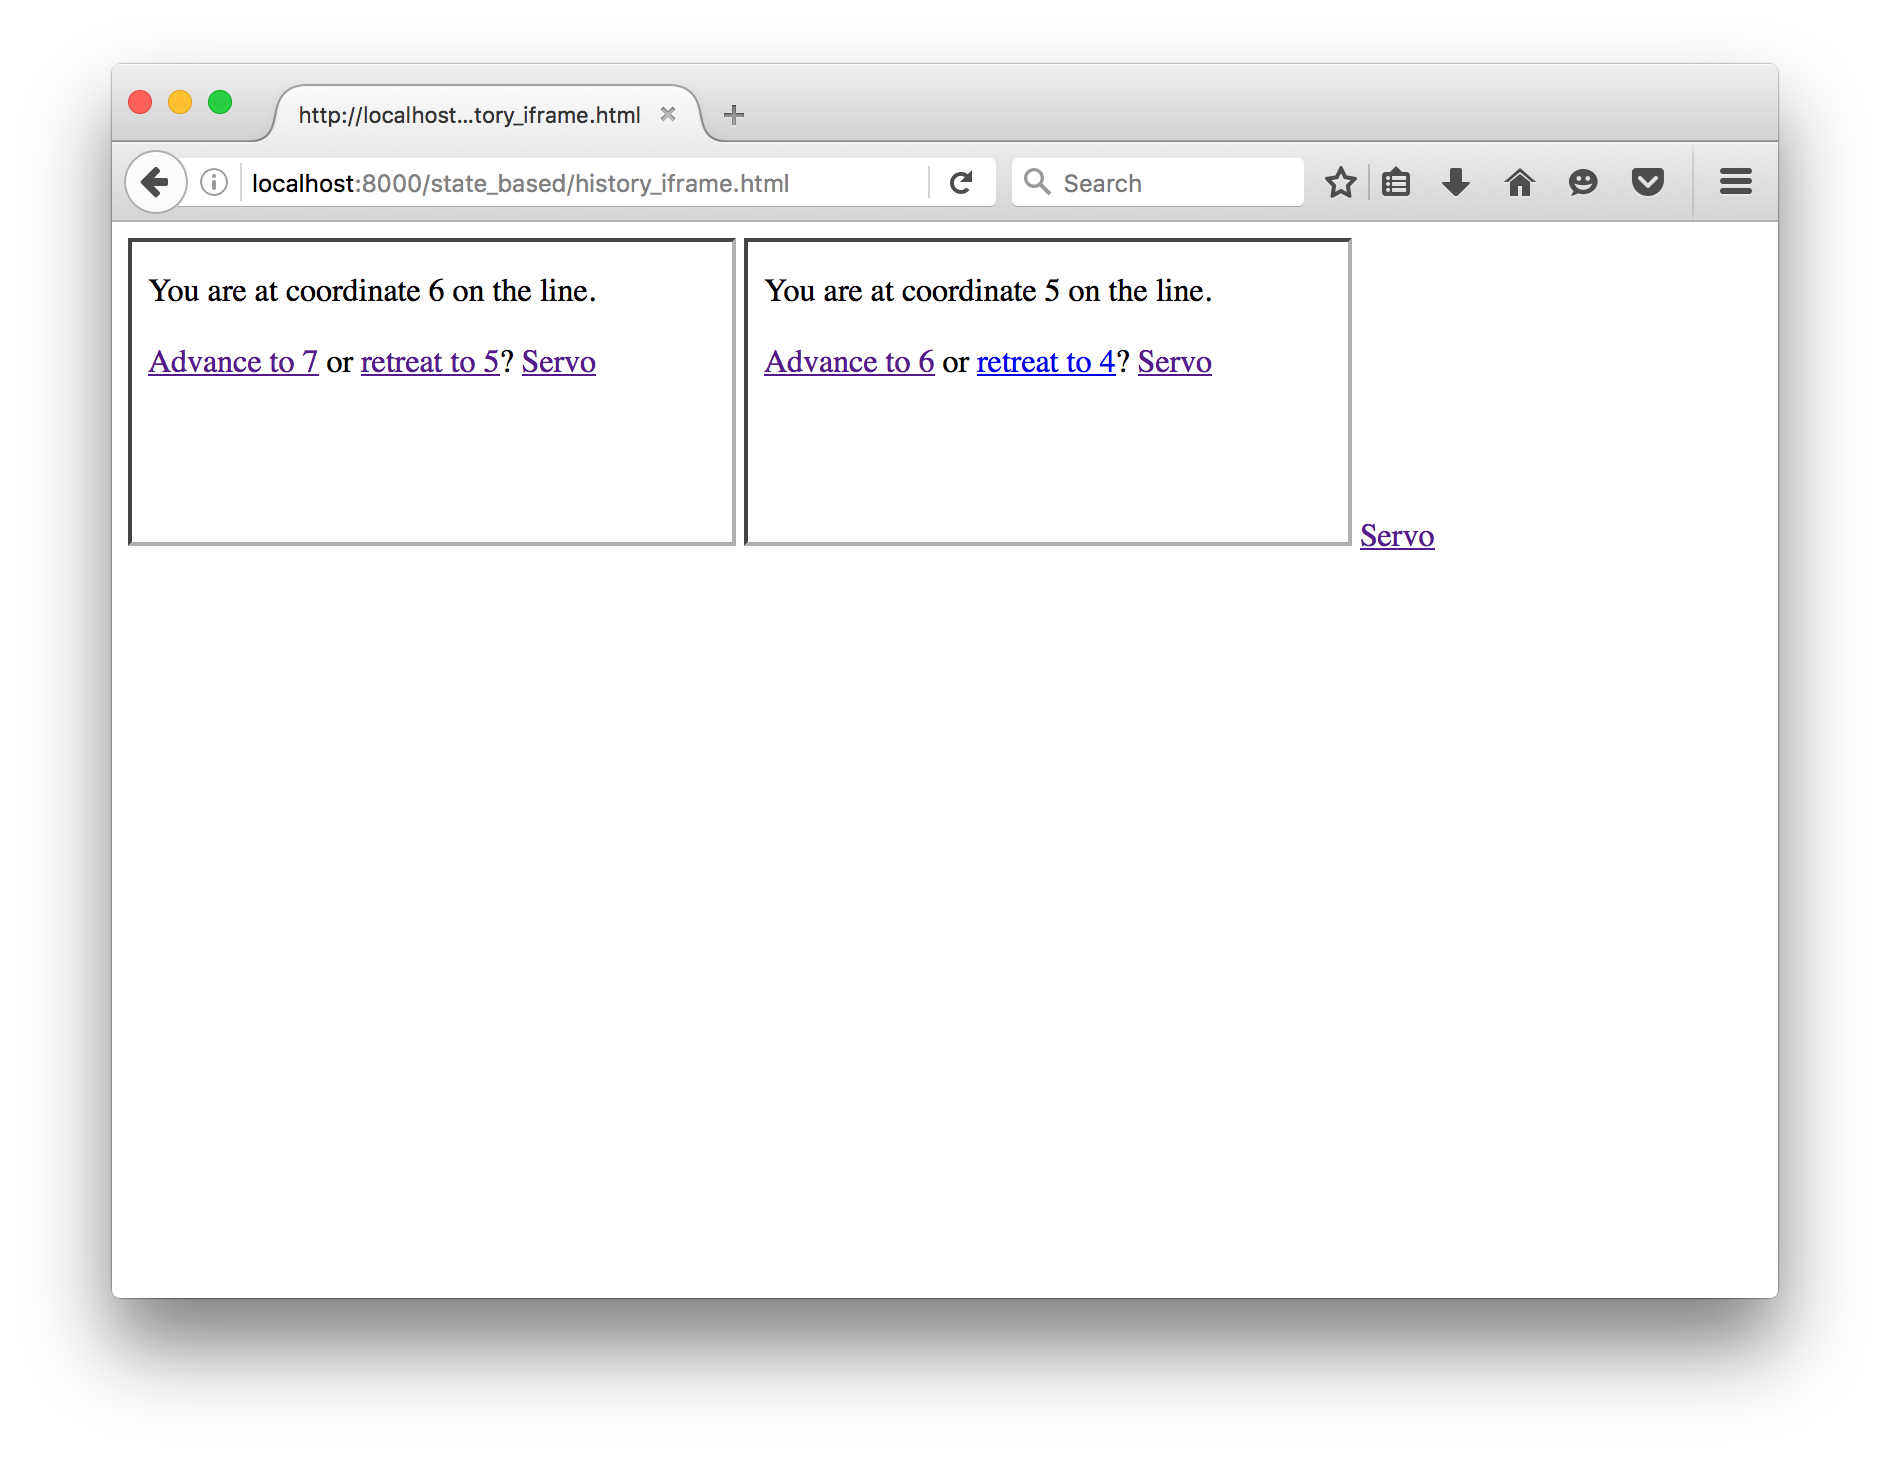
\includegraphics[width=.5\linewidth]{images/experiments/forwardback4state/firefox/2.png}%
    }~\raisebox{-.5\height}{
      \begin{tikzpicture}
        \node[doc,active,fully](0) at (0,0){0};
        \node[doc](1) at (1,-1){1};
        \node[doc,active,fully](2) at (2,-2){2};
        \node[doc,jshactive,fully](3) at (3,-1){3};
        \node[draw,dotted,fit=(0)]{};
        \node[draw,dotted,fit=(1)(3)]{};
        \node[draw,dotted,fit=(2)]{};
        \draw[->](0)--(3);
        \draw[->](0)to[out=-20,in=90](2);
      \end{tikzpicture}
    }
    \caption{Advance document 1 to $6$}
  \end{figure}

  Advance document 3 to $7$:
  \begin{figure}[H]
    \raisebox{-.5\height}{
      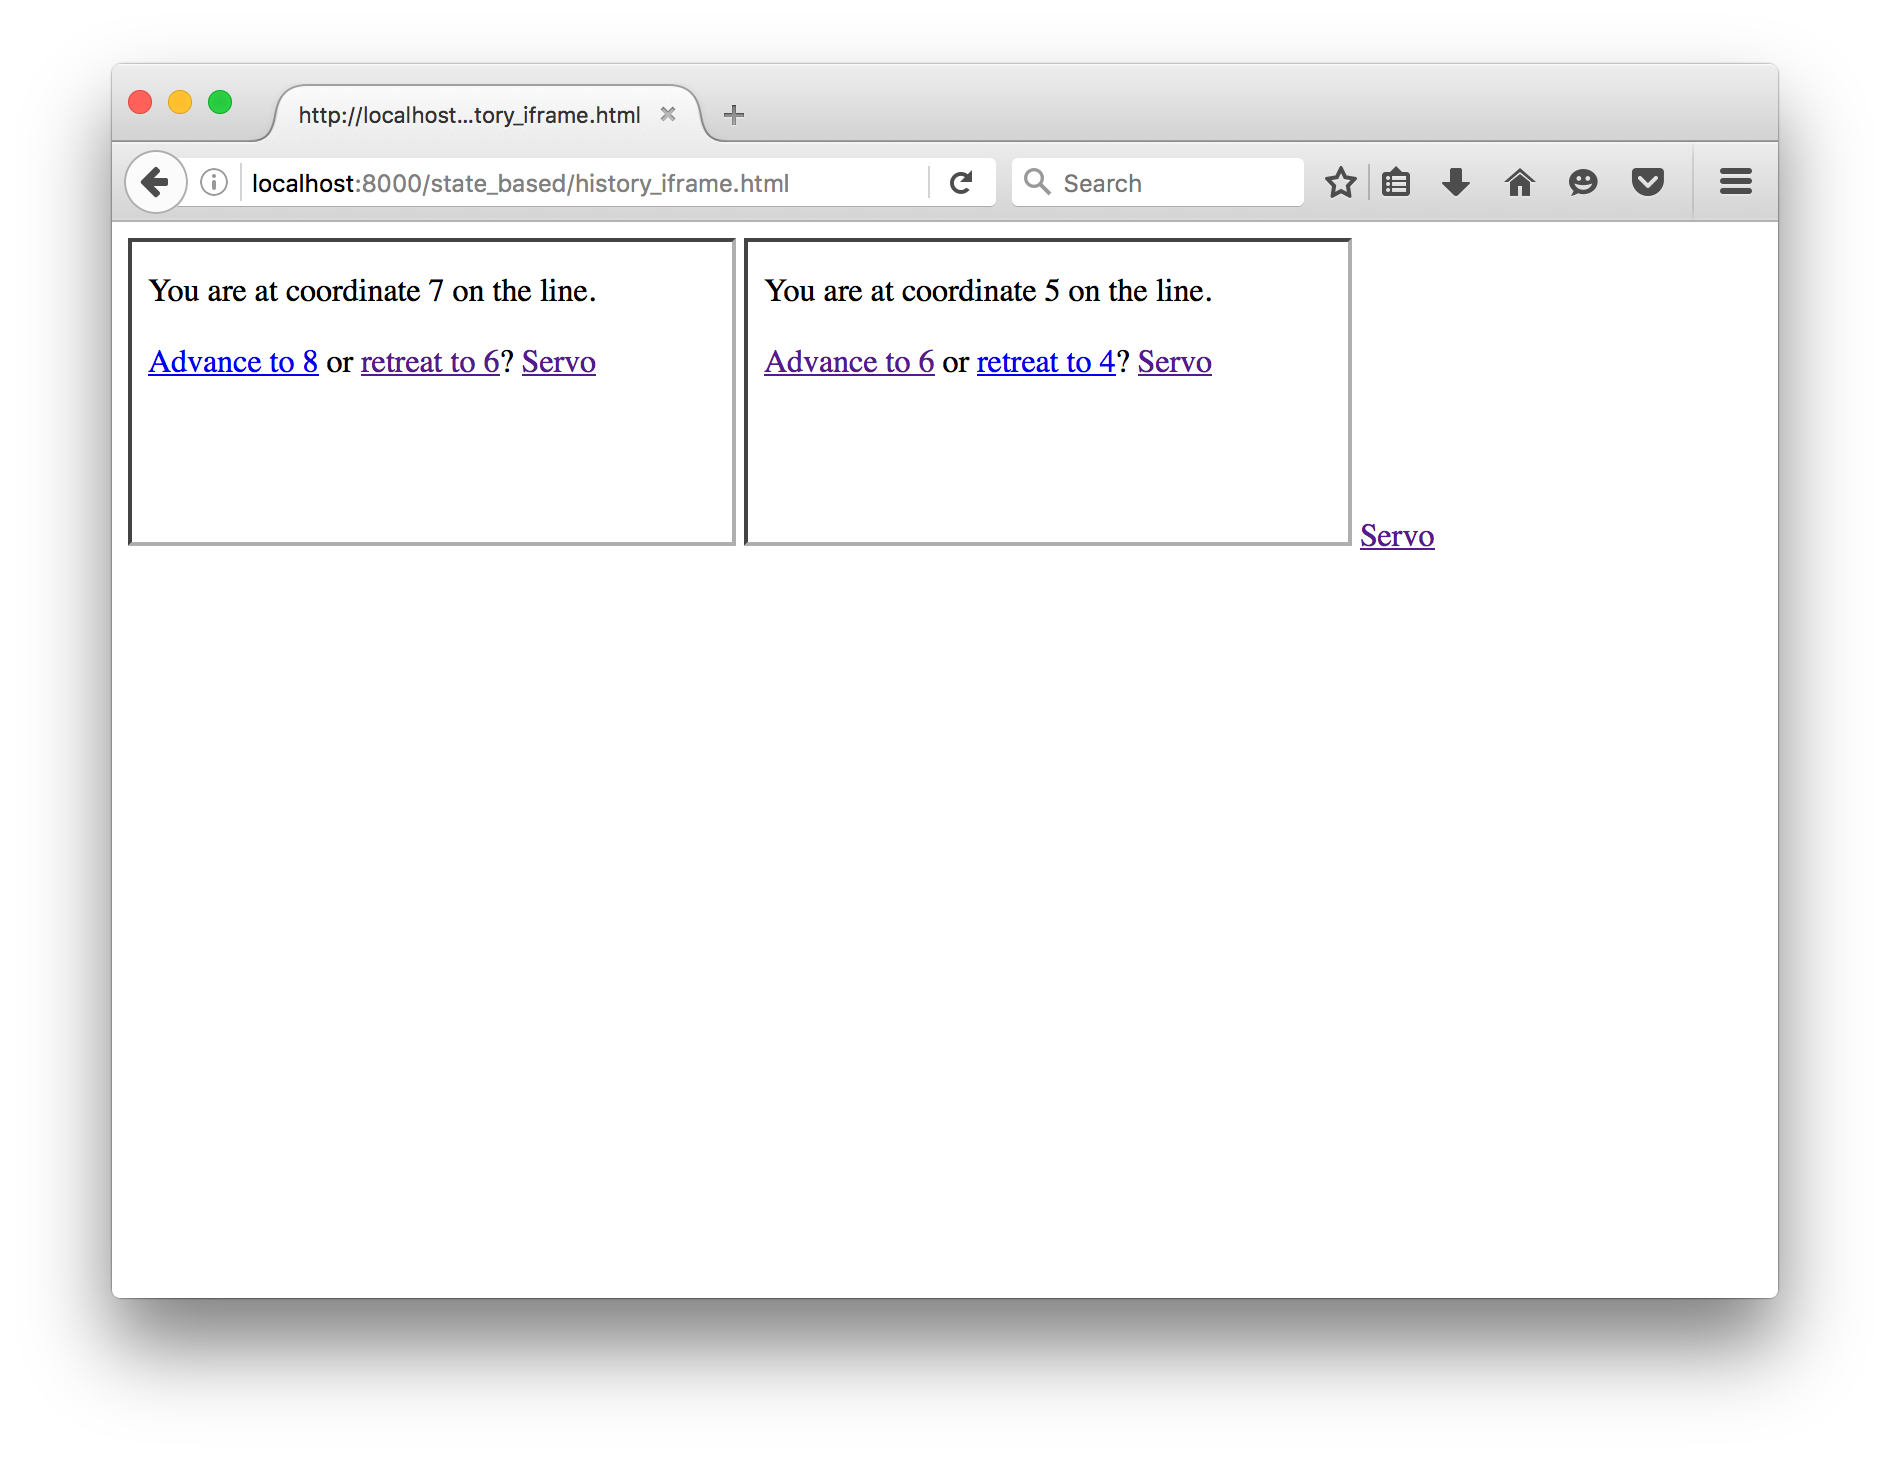
\includegraphics[width=.5\linewidth]{images/experiments/forwardback4state/firefox/3.png}%
    }~\raisebox{-.5\height}{
      \begin{tikzpicture}
        \node[doc,active,fully](0) at (0,0){0};
        \node[doc](1) at (1,-1){1};
        \node[doc,active,fully](2) at (2,-2){2};
        \node[doc](3) at (3,-1){3};
        \node[doc,jshactive,fully](4) at (4,-1){4};
        \node[draw,dotted,fit=(0)]{};
        \node[draw,dotted,fit=(1)(4)]{};
        \node[draw,dotted,fit=(2)]{};
        \draw[->](0)to[out=0,in=140](4);
        \draw[->](0)to[out=-20,in=90](2);
      \end{tikzpicture}
    }
    \caption{Advance document 3 to $7$}
  \end{figure}

  Advance document 2 to $6$:
  \begin{figure}[H]
    \raisebox{-.5\height}{
      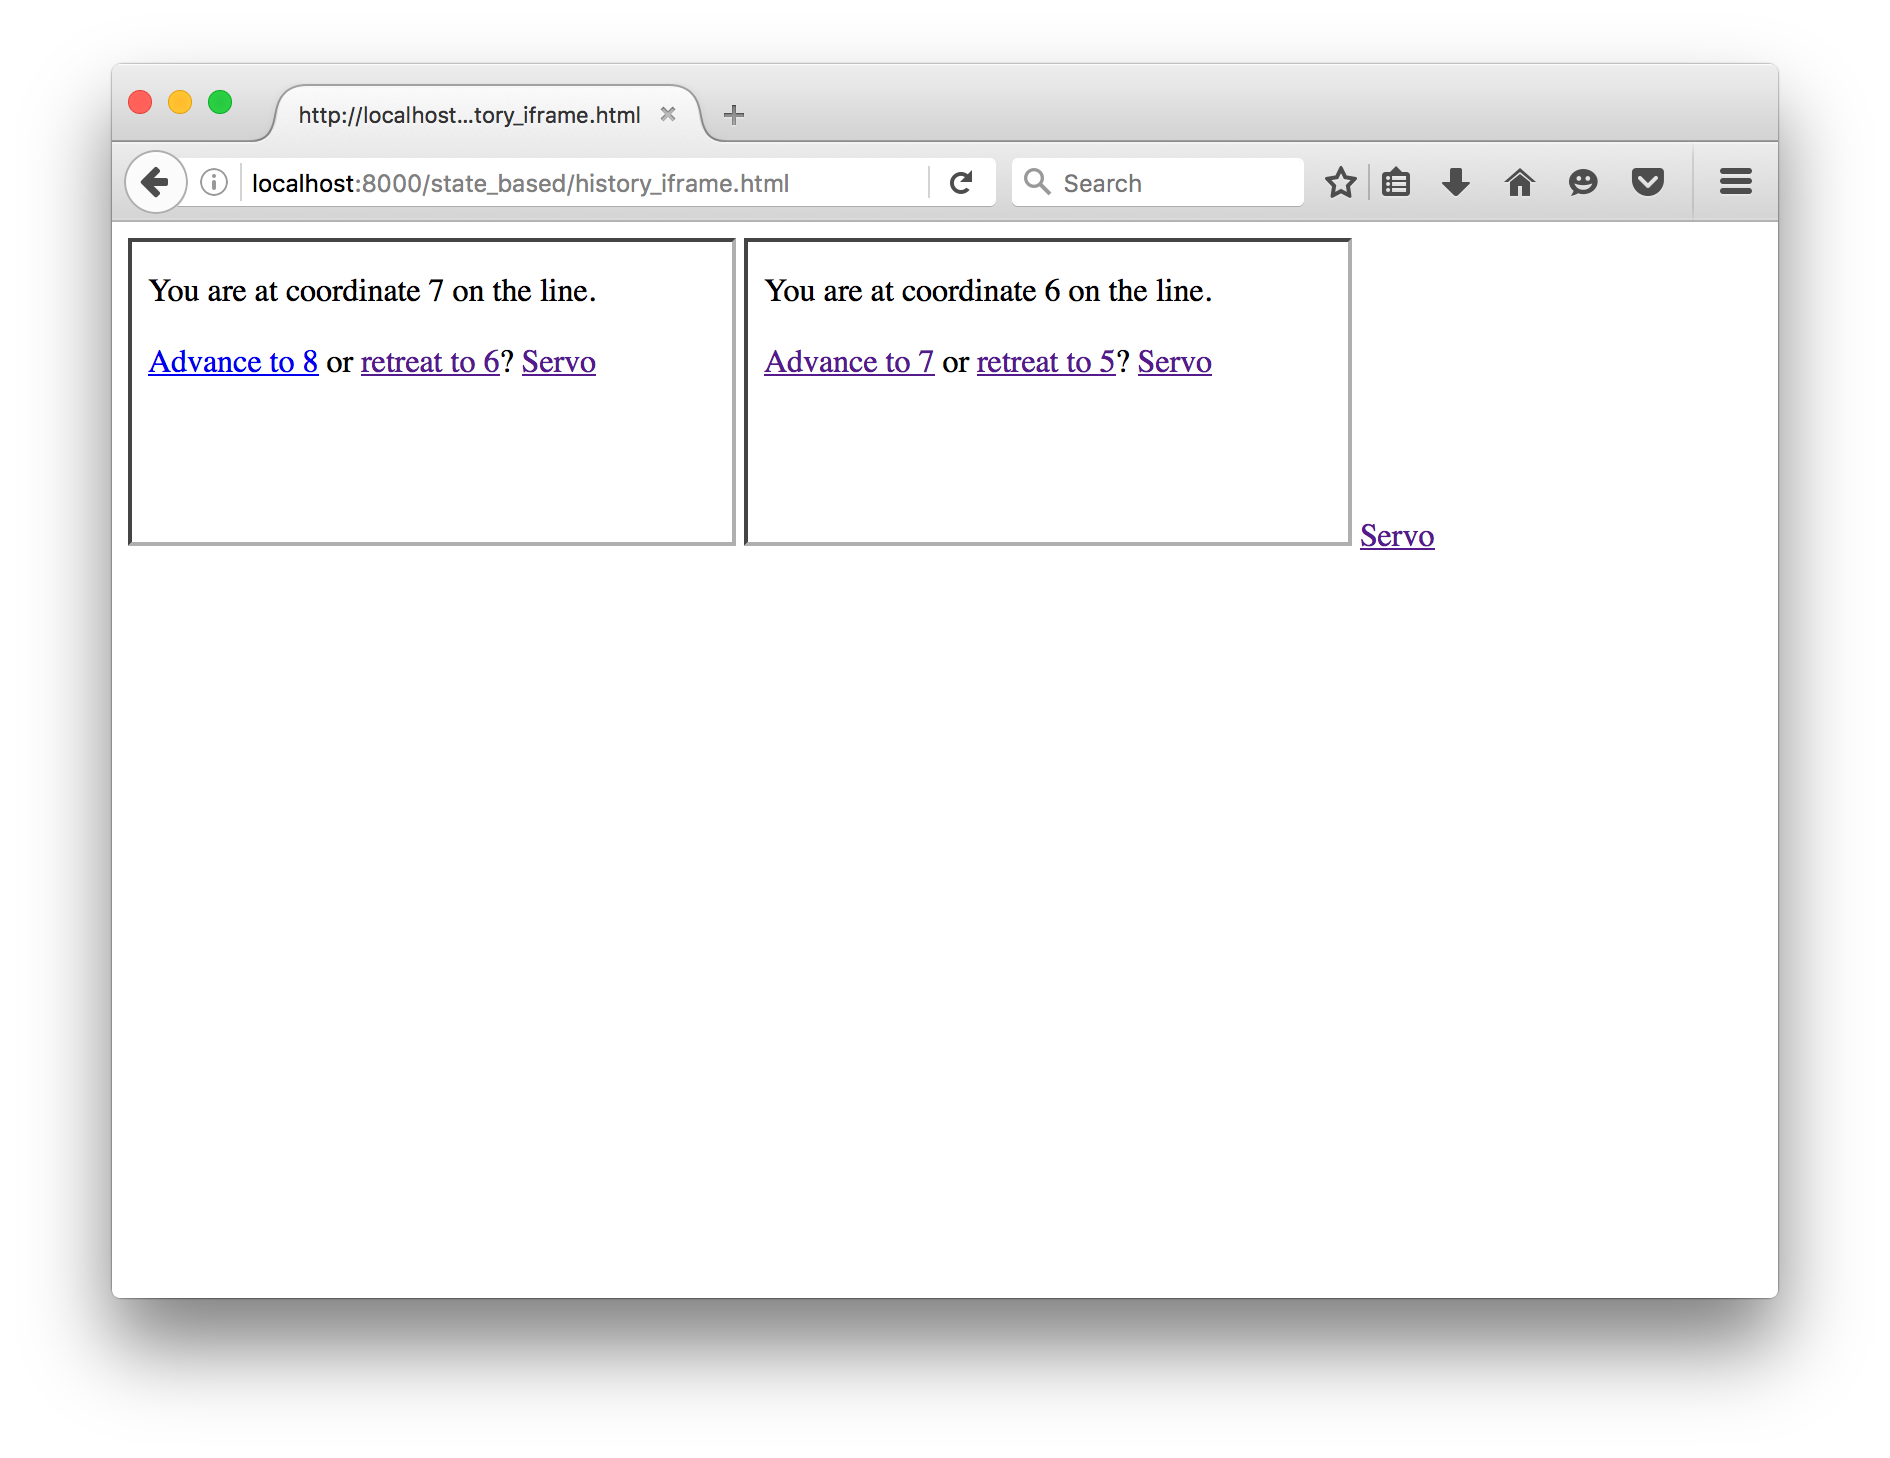
\includegraphics[width=.5\linewidth]{images/experiments/forwardback4state/firefox/4.png}%
    }~\raisebox{-.5\height}{
      \begin{tikzpicture}
        \node[doc,active,fully](0) at (0,0){0};
        \node[doc](1) at (1,-1){1};
        \node[doc](2) at (2,-2){2};
        \node[doc](3) at (3,-1){3};
        \node[doc,active,fully](4) at (4,-1){4};
        \node[doc,jshactive,fully](5) at (5,-2){5};
        \node[draw,dotted,fit=(0)]{};
        \node[draw,dotted,fit=(1)(4)]{};
        \node[draw,dotted,fit=(2)(5)]{};
        \draw[->](0)to[out=0,in=140](4);
        \draw[->](0)to[out=0,in=90](5);
      \end{tikzpicture}
    }
    \caption{Advance document $2$ to $6$}
  \end{figure}

  Advance $document 2$ to $7$:
  \begin{figure}[H]
    \raisebox{-.5\height}{
      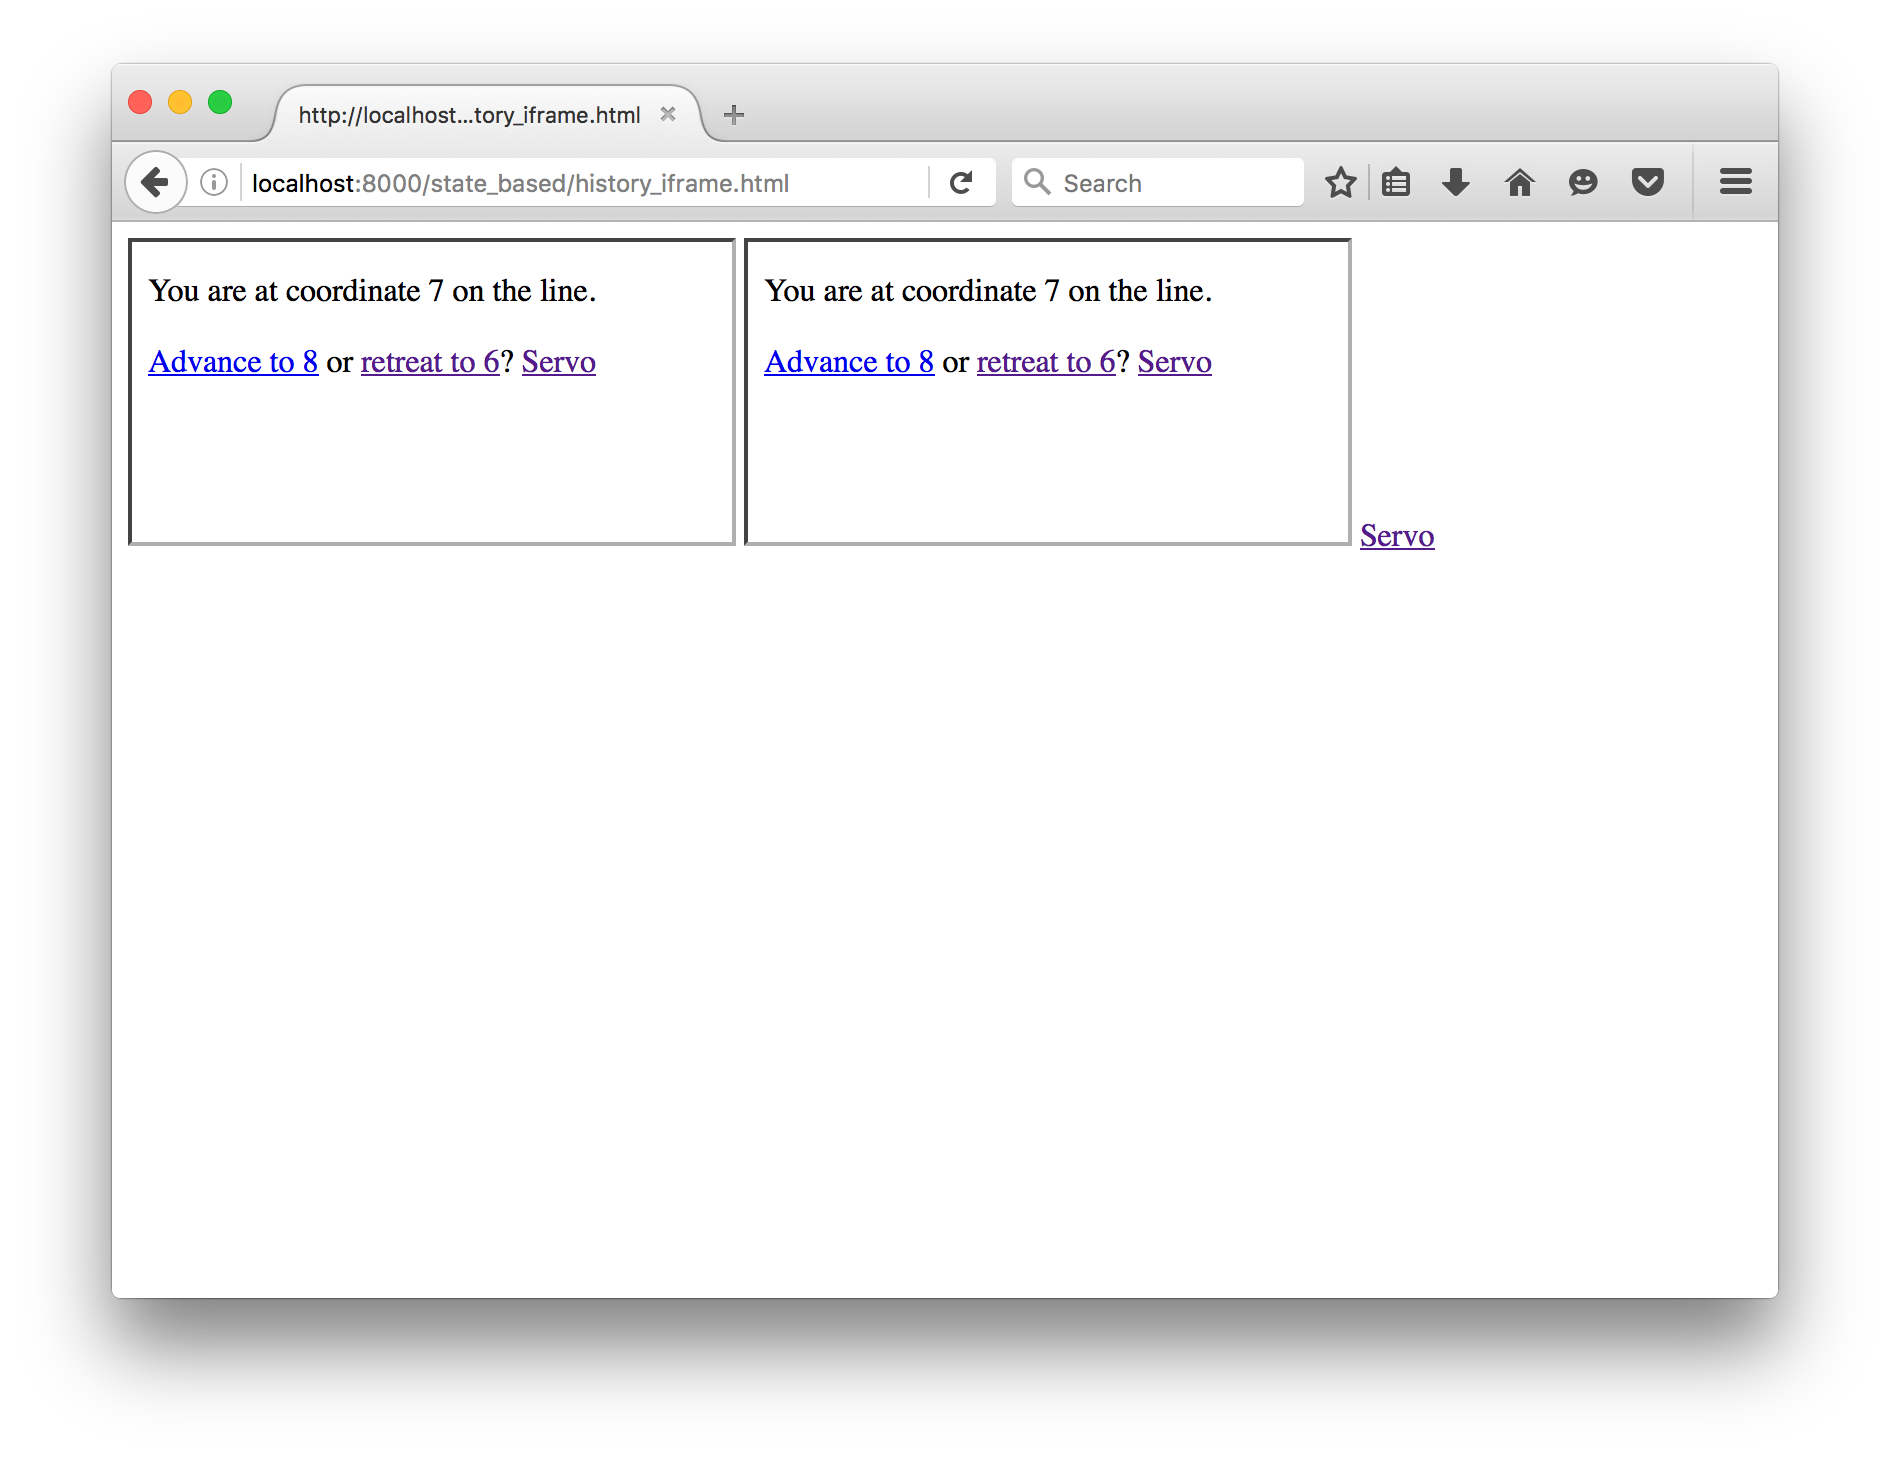
\includegraphics[width=.5\linewidth]{images/experiments/forwardback4state/firefox/5.png}%
    }~\raisebox{-.5\height}{
      \begin{tikzpicture}
        \node[doc,active,fully](0) at (0,0){0};
        \node[doc](1) at (1,-1){1};
        \node[doc](2) at (2,-2){2};
        \node[doc](3) at (3,-1){3};
        \node[doc,active,fully](4) at (4,-1){4};
        \node[doc](5) at (5,-2){5};
        \node[doc,jshactive,fully](6) at (6,-2){6};
        \node[draw,dotted,fit=(0)]{};
        \node[draw,dotted,fit=(1)(4)]{};
        \node[draw,dotted,fit=(2)(6)]{};
        \draw[->](0)to[out=0,in=140](4);
        \draw[->](0)to[out=0,in=120](6);
      \end{tikzpicture}
    }
    \caption{Advance document 2 to $7$}
  \end{figure}

  Traverse $\aNH$ by $-4$:
  \begin{figure}[H]
    \raisebox{-.5\height}{
      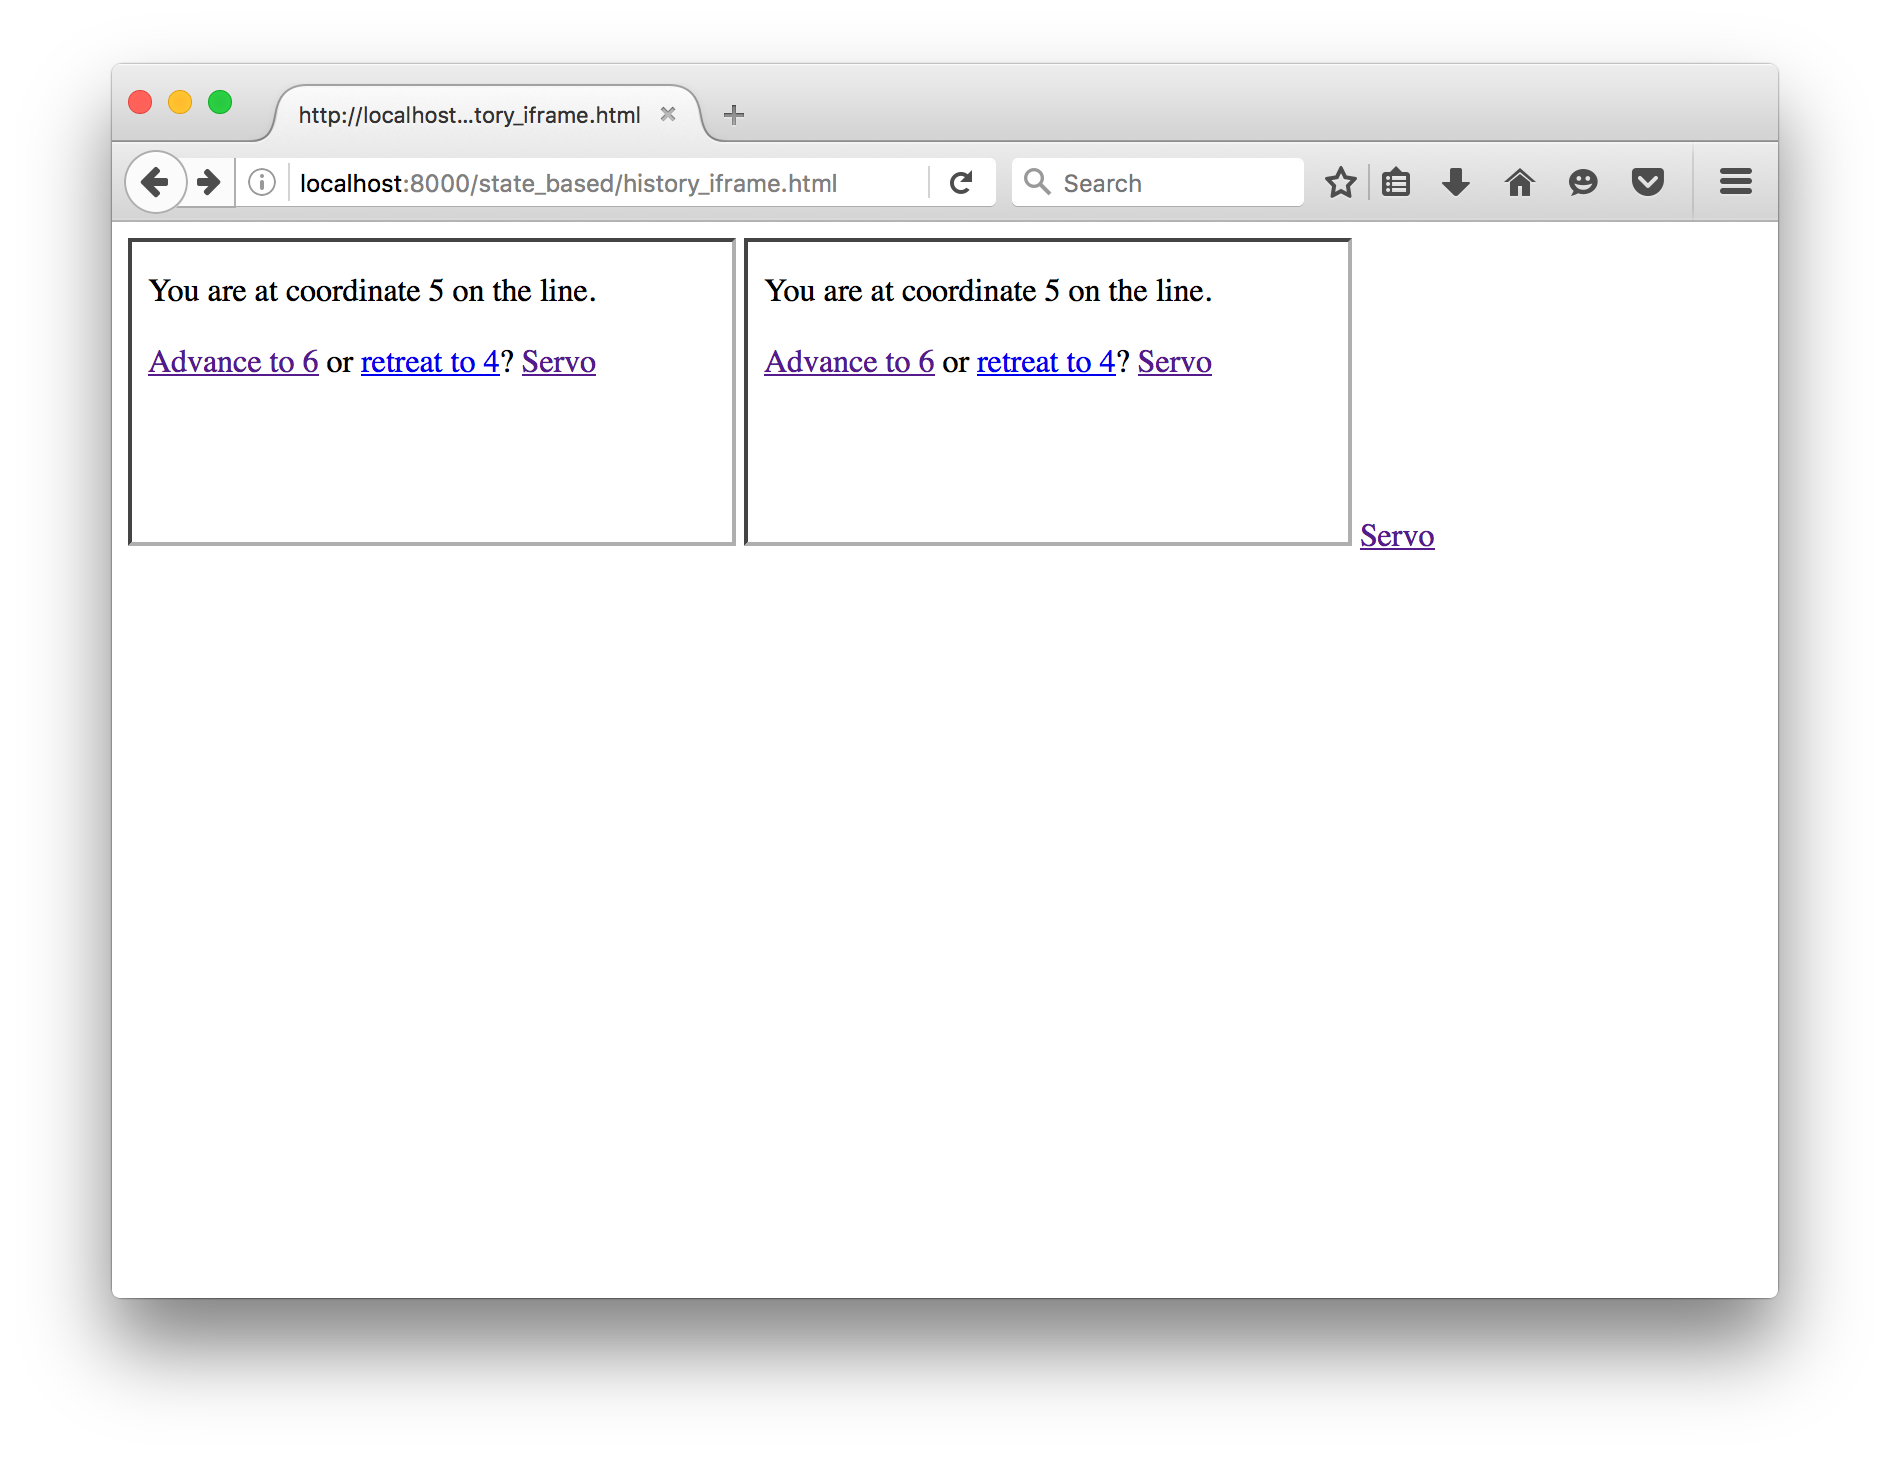
\includegraphics[width=.5\linewidth]{images/experiments/forwardback4state/firefox/6.png}%
    }~\raisebox{-.5\height}{
      \begin{tikzpicture}
        \node[doc,active,fully](0) at (0,0){0};
        \node[doc,active,fully](1) at (1,-1){1};
        \node[doc,jshactive,fully](2) at (2,-2){2};
        \node[doc](3) at (3,-1){3};
        \node[doc](4) at (4,-1){4};
        \node[doc](5) at (5,-2){5};
        \node[doc](6) at (6,-2){6};
        \node[draw,dotted,fit=(0)]{};
        \node[draw,dotted,fit=(1)(4)]{};
        \node[draw,dotted,fit=(2)(6)]{};
        \draw[->](0)--(1);
        \draw[->](0)to[out=-20,in=90](2);
      \end{tikzpicture}
    }
    \caption{Traverse $\aNH$ by $-4$}
  \end{figure}

  Traverse $\aNH$ by $4$:
  \begin{figure}[H]
    \raisebox{-.5\height}{
      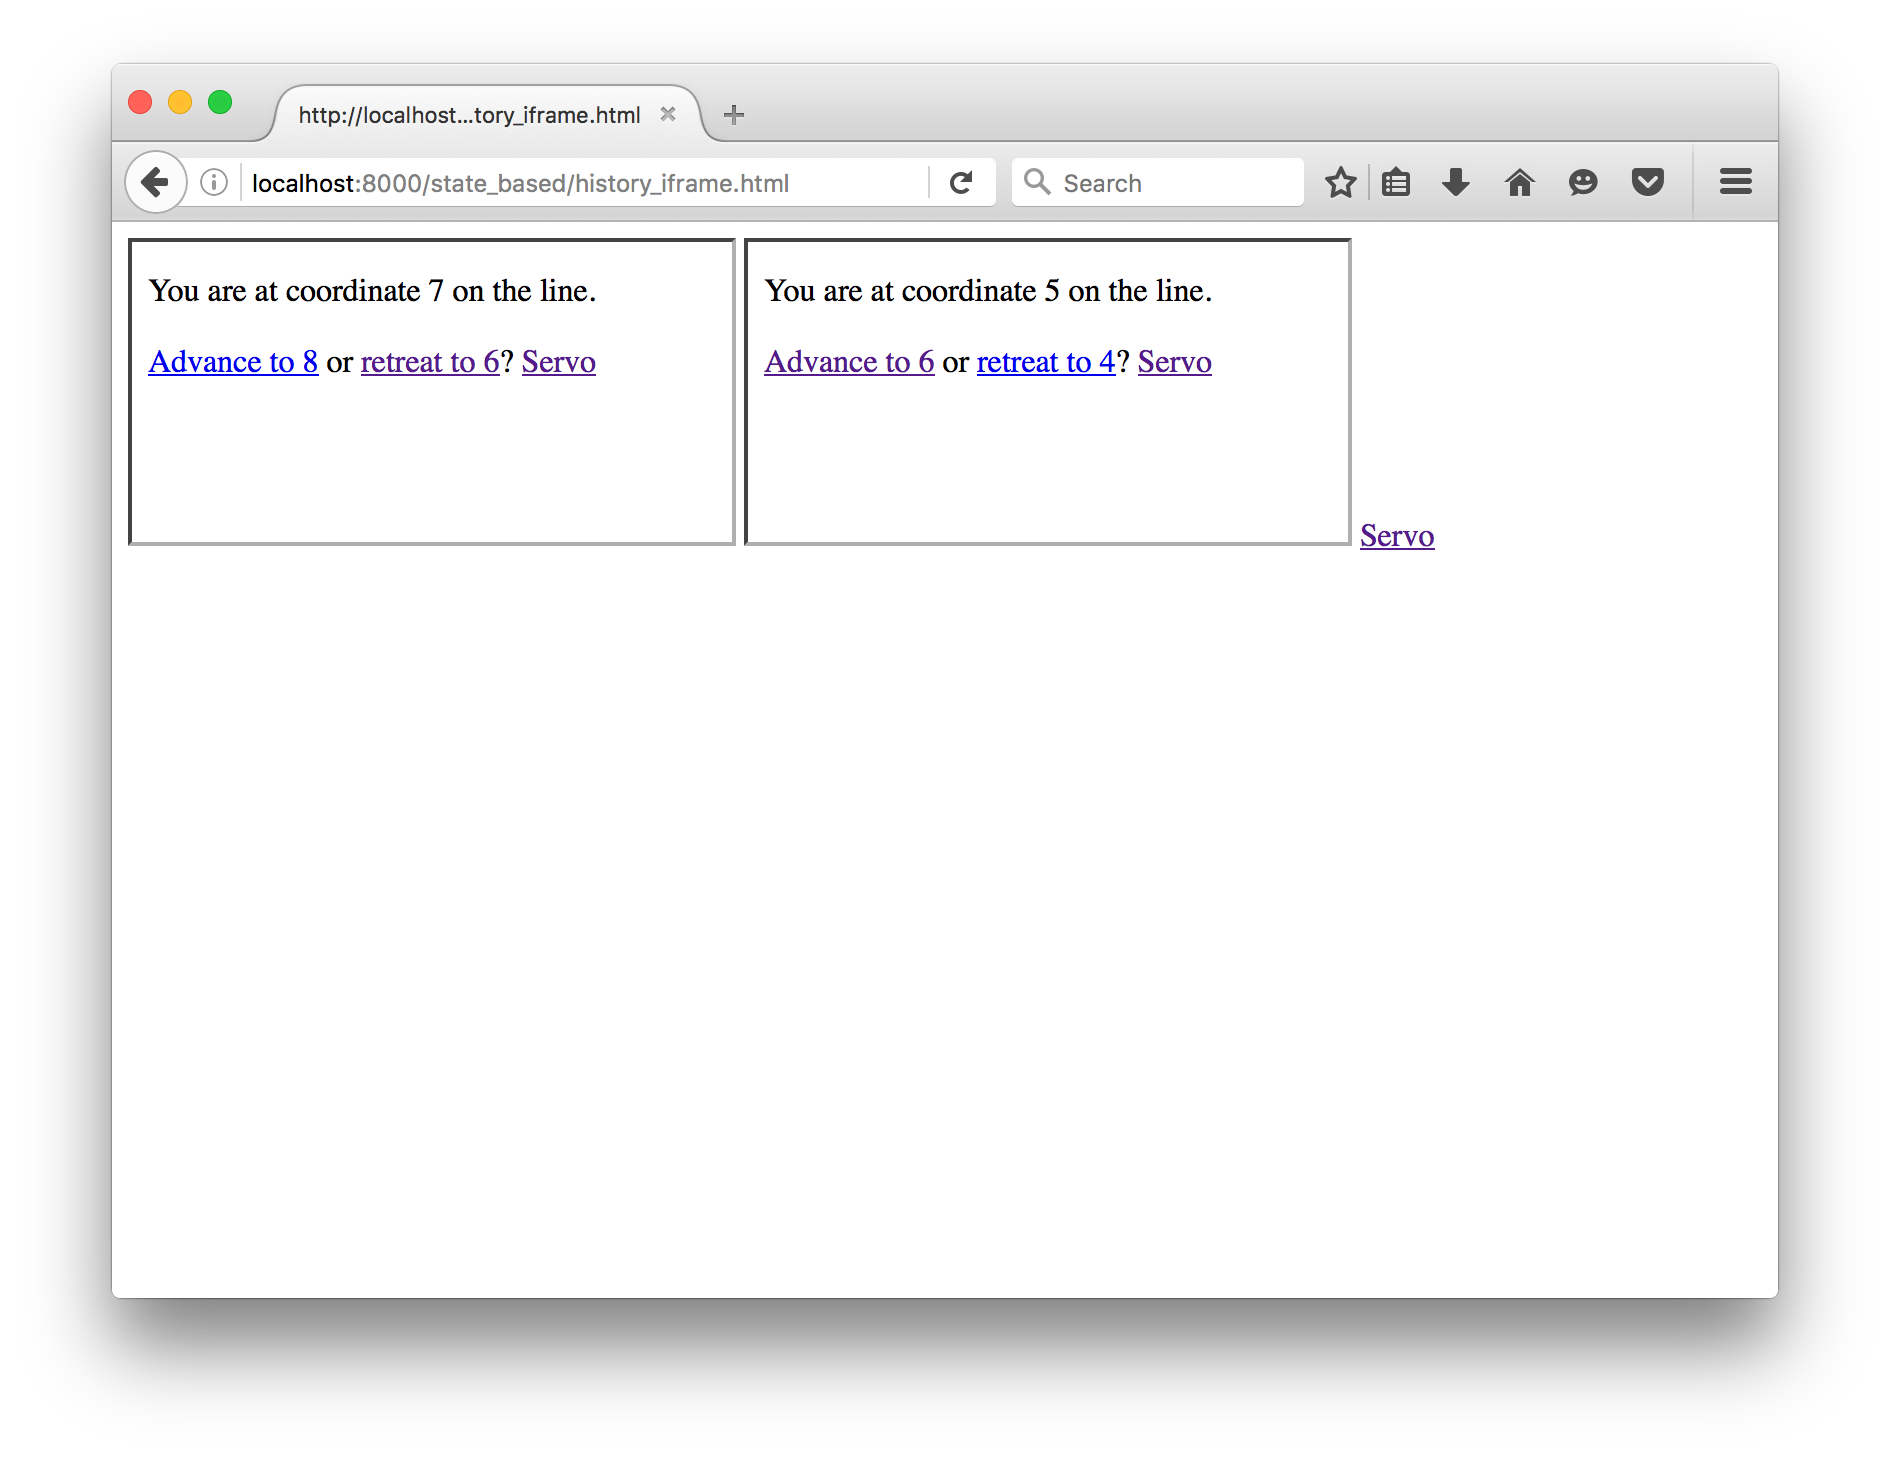
\includegraphics[width=.5\linewidth]{images/experiments/forwardback4state/firefox/7.png}%
    }~\raisebox{-.5\height}{
      \begin{tikzpicture}
        \node[doc,active,fully](0) at (0,0){0};
        \node[doc](1) at (1,-1){1};
        \node[doc](2) at (2,-2){2};
        \node[doc](3) at (3,-1){3};
        \node[doc,active,fully](4) at (4,-1){4};
        \node[doc](5) at (5,-2){5};
        \node[doc,jshactive,fully](6) at (6,-2){6};
        \node[draw,dotted,fit=(0)]{};
        \node[draw,dotted,fit=(1)(4)]{};
        \node[draw,dotted,fit=(2)(6)]{};
        \draw[->](0)to[out=0,in=140](4);
        \draw[->](0)to[out=0,in=120](6);
      \end{tikzpicture}
    }
    \caption{Traverse $\aNH$ by $4$}
  \end{figure}

  In this experiment, Chrome meets Goal~\ref{goal:homomorphism}.

\end{experiment}
